
%\documentclass[DIV19]{scrartcl}
%\usepackage[paper size={90mm, 120mm},left=2mm,right=2mm,top=2mm,bottom=2mm,nohead]{geometry}
% FIXME try prettyref
\documentclass[oneside,a4paper,12pt,BCOR20mm,DIV14]{scrbook}
%\documentclass{book}
% this gives a bit more than 2cm margin right and 4cm left
% koma-script.pdf: A4 is 210mmx297mm, BCOR is substraced before the page
% width is divided into DIV parts (HLU), a one sided leaves 1.5 HLU
% HLU*DIV=210-BCOR -> DIV=(210-BCOR)/HLU
% I want BCOR= 20mm 1.5 HLU = 20 mm 
% -> DIV=truncate(190*1.5/20) = truncate(14.25)=14
% I could use headinclude so that the header isn't printed into the margin

% Initially two softbound theses should be submitted to the
% Examinations Office for the examiners. Softbound theses should have
% the pages glued in.
% They don't need gold lettering on the spine.

\usepackage[utf8]{inputenc}
%\usepackage[T1]{fontenc}
\usepackage[usenames,dvipsnames]{color}
\usepackage[onehalfspacing]{setspace} 
\usepackage{graphicx}
\usepackage{longtable}
\usepackage{float}
\usepackage{wrapfig}
\usepackage{soul}
\usepackage{amssymb}
\usepackage{amsmath}

\usepackage[hypertex,breaklinks]{hyperref} % breaklinks only seems to
                                           % work with dvipdfm,
                                           % otherwise urls have no
                                           % line breaks
\usepackage{units}
\usepackage[disable]{todonotes} % for draft, disable for final
\usepackage{refcheck} % for draft, uncomment for final
\usepackage{lineno}
\usepackage{nomencl}
%\special{background Black}\special{color Green}
%\usepackage[utf8x]{inputenc} 
%\usepackage[T2A]{fontenc} % for the russian reference
\usepackage{wasysym} %diameter
% http://www.andy-roberts.net/misc/latex/latextutorial3.html

%\usepackage{url} % natbib.pdf p.11 break urls up, seems to be done
                 % with hyperref, though

\usepackage{natbib}


% for app_hilo
\usepackage{listings}
\usepackage{color}
\usepackage{textcomp}
\usepackage{subfigure}

% \listfiles % show which files are loaded by tex

\bibpunct{(}{)}{;}{a}{}{,}
\makenomenclature
\newcommand{\vect}[1]{\mathbf{#1}}
\renewcommand{\r}{\vect r}
\renewcommand{\a}{\vect a}
\newcommand{\s}{\vect s}
\def\k{\vect k}
\def\d{\vect d}
\def\e{\vect e}
\def\f{\vect f}
\def\c{\vect c}
\def\x{\vect x}
\def\y{\vect y}
\def\z{\vect z}
\def\q{\vect q}
\def\p{\vect p}
\def\l{\vect l}

\newcommand{\nvect}[1]{\vect{\hat{#1}}}
%\renewcommand{\i}{\nvect i}
\newcommand{\vi}{\nvect \i}
\def\hc{\nvect c}
\def\hs{\nvect s}
\def\hd{\nvect d}
\def\hx{\nvect x}
\def\hy{\nvect y}

\def\hz{\nvect z}
\def\n{\nvect n}
\def\t{\nvect t}
\def\m{\nvect m}
\def\vrho{\boldsymbol\rho}
\def\abs#1{\mathopen| #1 \mathclose|}

\newcommand{\bild}[1]{\includegraphics[width=12cm]{#1}}

\DeclareMathOperator{\sign}{sign}
\DeclareMathOperator*{\sinc}{sinc}

% reference to picture
\newcommand{\figref}[1]{\figurename~\ref{#1}}
\title{sbl}
\author{nal}
% short summary at the beginning of a section
\newenvironment{summary}{\begin{quote}\small}{\end{quote}}
%\includeonly{state-of-the-art}
\begin{document}
\listoftodos
%\linenumbers
\begin{titlepage}
  
  \hspace{-4cm}
  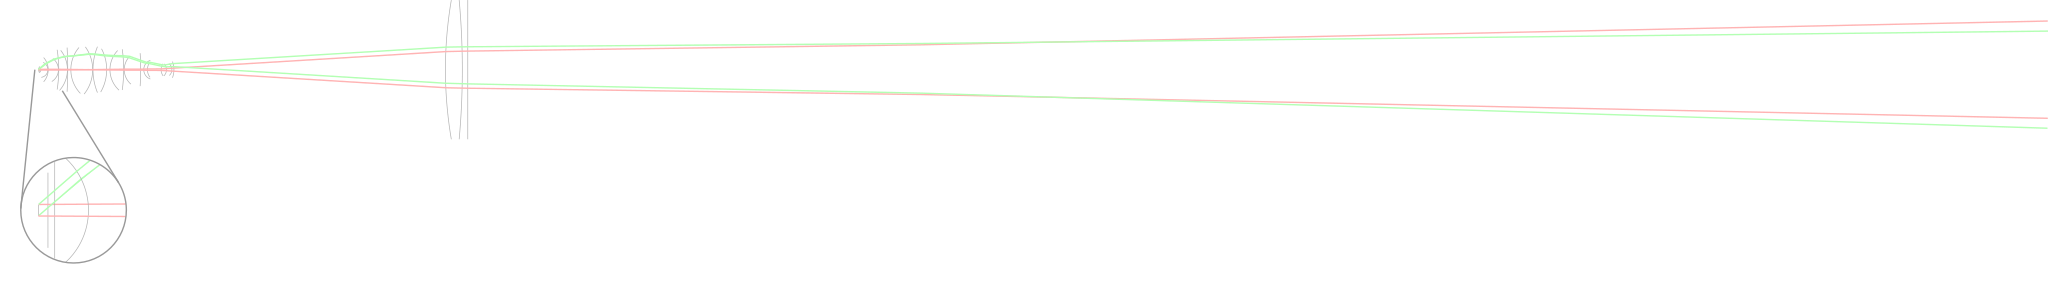
\includegraphics{objective-trace}



  \vspace{-5cm}
  
  \hspace{4cm}\textsf{\Huge Spatio--Angular Microscopy}
  
  \vspace{2cm}
  \hspace{6cm}\textsf{\huge PhD Thesis}


  \vspace{3cm}
  \hspace{4cm}\textsf{\Large Martin Kielhorn}
  
  \vspace{1cm}
  \hspace{4cm}\textsf{\Large July 2012}
\end{titlepage}
\newpage
\section*{Abstract}
\begin{summary}
Photobleaching and phototoxicity pose a problem in live cell
imaging. Fluorescence imaging induces reactive oxygen species in
observed organisms which can alter the behaviour of the sample, and so
minimising light exposure is an important goal.

We augment a widefield epifluorescence microscope with two spatial
light modulators. By controlling the spatial illumination pattern and
the angle at which illumination occurs, we achieve control of the
illumination pattern in three dimensions.

Our custom software is used to obtain an initial image stack of the
specimen. Subsequent image sections are exposed with excitation
patterns that take into account the previous image stack. Depending on
the distribution of fluorophores this adaptive exposure can
considerably reduce photobleaching and phototoxicity.
\end{summary}

\urlstyle{sf}
%\setcounter{tocdepth}{3}
\section*{Preface}
\subsection*{Introduction}
In the work by \citet{Levoy2003}, a scene with a toy soldier behind a
plant is captured by a camera while being illuminated with sixteen
projectors.  Sophisticated illumination control allows them to
estimate a three-dimensional model of the scene and finally, they can
illuminate the toy without exposing the plant.

In our work we have adapted this idea for the field of fluorescence
microscopy. This is not as straightforward as it may seem.  The ideas
from \citet{Levoy2003} are based on ray optics and in extreme cases,
e.g.\ for very fine patterns, don't work for microscopes. Also, there
are related technical issues like the illumination, e.g.\ the light
source of a data projector usually doesn't have enough brightness to
illuminate a microscope efficiently.

Here we build a spatio-angular microscope. It contains two
programmable masks and can control the illumination angle for specific
spatial parts of the sample. The advantage of this microscope lies in
imaging of living samples with sparse, three-dimensionally extended
labelling.

In chapter \ref{sec:intro}, we introduce photophysics of fluorescence
and emphasize the importance of oxygen for phototoxicity. Furthermore,
we also explain conventional microscopes and CCD cameras.

In chapter \ref{sec:approaches}, we compare some state-of-the-art
techniques for illumination control in microscopes.  Particularly in
section \ref{sec:light-field-microscopy}, we discuss the micro-lens
based light field microscope by Levoy's computational photography
group, which imaged the toy soldier in 2003.

In chapter \ref{sec:setup}, we describe our microscope and in chapter
\ref{sec:experiments}, we show some images, taken with illumination
control in our prototype.

There is also an extensive appendix where we document more technical
issues like read noise calibration of a camera (Appendix
\ref{sec:ccd-meas}) or finding a rigid transform between a camera and
a display (Appendix \ref{sec:rigid}).

In the appendix, we also describe a completely different approach for
spatio--angular illumination based on holography (Appendix
\ref{sec:app_holo}) and we document an interferometric attempt to
convert our precise programmable phase mask into a spatial intensity
modulator (Appendix \ref{sec:app_dic}).

Note that the Appendix \ref{sec:dvi} describes a modification of our
prototype with a spatial light modulator that receives data from a
graphics card. A higher bandwidth makes this approach more useful than
the prototype described in the main text and we tried to implement
this first. However eventually, it proved too difficult to trigger the
components in this configuration and we switched to the more
predictable USB-controlled display as described in the main body of
the text.
 
The appendix also contains some theoretical explainations of
raytracing (Appendix \ref{sec:raytrace}), computational optical
sectioning (Appendix \ref{sec:app_hilo}) and the wave-optics based
simulation of our microscope (Appendix \ref{sec:sim-angle}).

\subsection*{Source Code Availability}

Source code that has been developed during this project is available
on \url{https://github.com/plops/mma}.  It contains implementations
for:
\begin{itemize}
\item illumination planning based on raytraces (see Appendix
  \ref{sec:raytrace})
\item moving the $z-$stage of a Zeiss Axiovert 200M microscope body
\item controlling an Andor Clara camera using the Andor SDK version
  2. For the other cameras following below, control software was written:
  \begin{itemize}
  \item Photometrics Cascade~II (interface to unsupported
    closed-source driver, only works on very old 32-bit Linux kernels)
  \item mvBlueFox 102G using the SDK
  \item Logitech Pro 9000 using a generic Video4Linux interface
  \item Andor sCMOS using Andor SDK version 3
  \end{itemize}
\item displaying patterns using a graphics card that supports OpenGL
  on a ForthDD SXGA ferroelectric LCoS display
\item controlling a stand-alone ForthDD WXGA 3DM display controller
  using USB
\item estimating the parameters of a rigid transformation between
  camera and LCoS display (see Appendix \ref{sec:rigid}),
\item controlling the micro-mirror array by Fraunhofer IPMS using
  their SDK
\item some specific image processing tools:
  \begin{itemize}
  \item three-dimensional convolution and Fourier transforms
  \item drawing of lines and ellipsoids in volumes
  \item rasterization of triangles (for creating shadow maps in the
    BFP, see section \ref{sec:trace-detect})
  \item calculation of optical transfer function for high NA
    objectives
  \item localization of spherical nuclei in volumetric data (parts of
    the algorithm as described in \citet{Santella2010})
  \end{itemize}
\end{itemize}
The main development was done using GNU~Linux. However, portability
was kept in mind and most of the code was made to work with Microsoft
Windows as well.

\subsection*{Acknowledgements}
It is my pleasure to thank all those who have made this thesis
possible. First and foremost, I owe my deepest gratitude to my
supervisor Rainer Heintzmann for giving me the opportunity to become
part of his research group at King's College London and later in the
Institute of Photonic Technology in Jena.

I owe my sincere thanks to Kai Wicker, Jakub Nedbal, Susan Cox, Daniel
Appelt, Ond\v rej Mandula, Ronny F\"orster, Ivana \v Sumanovac,
Eckhard Birkner, Kathrin Klehs and all the other members of our group
for valuable discussions, support and review of the manuscript.

My sincere thanks to the European Union Framework Programme 7 (project
number 2115597) for the studentship on this project.
I also thank Erhard Ipp, G\"unter Z\"ochling, Vincent Galy, QueeLim
Ch'ng, J\"org Heber, Mark Eckert, Dirk Berndt, Joel Seligson and
Jean-Yves Tinevez for helpful collaboration.   

Furthermore I highly appreciate the input of Miroslav Grajcar, Edward
Rosten, Christophe Rhodes, Paul Khuong, Nikodemus Siivola, Levente
M\'esz\'aros and Lu\' is Oliveira. Occasionally, the expertise and
insight of them steered me into right direction or greatly simplified
problems I faced.

Finally, I wish to thank the authors and contributors to the following
software projects: Linux, GCC, Emacs, SBCL \citep{Rhodes2008}, Maxima,
Micromanager \citep{Edelstein2010}, DIPimage, Wireshark, Latex,
Inkscape, Gimp, ImageJ/Fiji \citep{Abramoff,Schindelin2012} and
Blender.  These free software projects and their communities are
invaluable to my work and greatly enhance my efficiency.

The work presented in this thesis is my own, unless I cite a reference
to acknowledge data or images to a different author. In the rest of
the thesis I use the word ``we'', even though I did the work myself.

\begin{flushright}
  M.~K.
\end{flushright}

\noindent
Jena, Germany

\noindent
July 2012

\newpage
\tableofcontents
\printnomenclature
\newpage
\chapter{Introduction}
Fluorescence microscopy is an old technique that has been established
in live sciences for a long time. Being able to see things happening
at the micrometre scale is the fundamental path to understand life and
disease.

Innovation continuously improves microscopy and occasionally new
fields of research are opened up: The discovery and development of
fluorescent proteins initiated a revolution in how microscopy can be
applied in living specimen. 

Optical high resolution techniques allow
to observe biological processes at the scale of individual molecules
(tens of nm). 

Labels that report membrane potentials or viscosity within cells,
compounds that locally release chemicals when illuminated by light or
even ion pumps that can be switched by light promise novel interesting
research.

All these techniques have in common, that excitation light has to
reach a focal point, line or plane within the sample. For this the
light has to traverse a more or less dense distribution of
fluorophores.

With few exceptions (2-photon, SPIM, CLEM) microscopes are generally
not optimized for exciting only the in focus fluorophores.

Here we build a spatio-angular microscope. It contains two
programmable masks and can control which parts of the sample (spatial)
are illuminated by what angles. The advantages of this microscope lie
in imaging of living samples with sparse, three-dimensionally
extended labelling.
\newpage

\section{Conventional microscopes}
\begin{summary}
  Microscopes that are in common use today do not optimally excite
  fluorophores within the specimen. In this section we outline how
  these microscopes work. We explain how out-of-focus blur severely
  limits the performance of the widefield microscope. Then we discuss
  how confocal microscopy improves the sectioning capability at the
  cost of increasing the phototoxic load on the specimen.
\end{summary}
The basic building block of microscopes are lenses. A lens is a piece
of glass with two polished spherical (a shape of lower symmetry is
much harder to manufacture) surfaces. Light is slower in glass than in
air. The shape of a lens redirects photons and the thickness of the
material can delay them. A lens focuses a parallel beam of light into
a spot on its focal plane. The distance between focal plane and the
region where the rays start to converge is called focal length.
\begin{figure}[!hbt]
  \centering
  \input{widefield-microscope.eps_tex}
  \caption{{\bf a)} Schematic of a modern microscope. The sample is in
    the front focal plane of the objective. The detection tubelens TL1
    forms a magnified image on the camera. {\bf b)} Widefield
    epifluorescence excitation. The excitation tubelens focuses a
    laser into the back focal plane (BFP). The beam is reflected by a
    dichroic beam splitter (BS) towards the objective. An extended
    area in the specimen is illuminated. Fluorescence light of lower
    wavelength returns through the objective, is transmitted through
    BS and forms an image on the camera. {\bf c)} Confocal
    microscope. A pinhole PH2 is imaged as a diffraction limited spot
    into the specimen. Returning fluorescence light is only detected
    when it passes through an aligned pinhole PH1. This configuration
    rejects light that doesn't originate from the front focal plane
    (green) of the objective.}
  \label{fig:widefield-microscope}
\end{figure}

The yellow beam in \figref{fig:widefield-microscope}~a) represents
rays that start from the intersection $O$ of the optical axis and the
front focal plane of the objective. The objective collects the rays
and collimates them into a beam that is parallel to the optical
axis. After traversing the tube length $f+f_\textrm{TL}$ the detection
tube lens TL1 focuses the rays on the intersection $O'$ of its focal
plane (the intermediate image plane) and the optical axis.

The blue beam corresponds to rays that start from an off-axis point
$P$ in the front focal plane of the objective. Behind the objective
the blue beam is a parallel beam. However, the beam isn't parallel to
the optical axis. The tube lens TL1 focuses the blue beam into a spot
at $P'$ on its focal plane. Using the theorem of intercepting lines
one obtains for the magnification $M$:
\begin{align}
  M=\frac{\overline{O'P'}}{\overline{OP}}=\frac{f_\textrm{TL}}{f}.
\end{align}
In our microscope we use an objective with magnification $M=63$. The
focal length of the tube lens is \unit[164.5]{mm} for most Zeiss
microscopes. Therefor the focal length of our objective is
$f=\unit[2.61]{mm}$.

Assuming we have a metal mirror with two small
($\diameter<\unit[120]{nm}$) holes in the reflective coating with
$\unit[2]{\mu m}$ distance between them.  We put this object into the
front focal plane of the objective and position a camera on $O'$. When
illuminating the mirror from the side opposite to the objective, the
camera will show two spots with $\unit[126]{\mu m}$ distance.

Note that \figref{fig:widefield-microscope} depicts a thin-lens
model. A real objective contains in the order of ten coated lenses of
different glass and crystalline materials. Their curvatures, positions
and materials were all carefully chosen, taking into account
manufacturing tolerances and wavelengths, so that the microscope
behaves exactly as the thin-lens model predicts. Diffraction defines
how well objective and thin-lens model have to match.

It is quite possible that heating to \unit[37]{${}^\circ$C} will ruin
such a high-precision instrument. A related source of aberrations
(departure of design performance) is the refractive index inside of
the specimen. Later in this work \todo{add reference} %FIXME reference
we will describe a more complicated model that can predict the effect
of embedding the sample in water (instead of immersion oil with the
same refractive index as the glass).

\subsection{Widefield epifluorescence microscope}
Fluorescence photons are emitted in all directions, independent of the
original illumination direction. Therefor it is convenient to use the
objective for excitation as well as detection. This mode of microscopy
is called epifluorescence (Greek: $\varepsilon\pi\iota$; on, above).
One advantage is that even (the frontal side of) opaque specimen can
be imaged. Furthermore it is beneficial that the illumination needs to
be aligned only once.

\nomenclature{BFP}{Back focal plane}

The red beam in \figref{fig:widefield-microscope}~b) is a parallel
laser. The excitation tube lens TL2 focuses the beam into the back
focal plane (BFP) of the objective. The beam is reflected at a
dichroic beam splitter (BS). This is a glass plate that has been
coated with dielectric layers. The refractive index, thickness and
sequence of the layers are designed so that the excitation light is
reflected towards the objective but lower energy fluorescence light
returning from the objective is transmitted towards the camera. Behind
the objective the beam is parallel and illuminates the specimen.
\subsubsection*{Non-uniformity due to coherent interference}
Note that tiny dirt particles and coherent interference in laser beams
can produce unwanted non-uniformities in the illumination. As a remedy
sometimes the spatial coherence of the laser is reduced. Often
incoherent light emitting diodes, mercury or xenon arc lamps are used
instead of lasers. In the latter case the dichroic beam splitter is
preceded by a band pass filter that selects the useful part of the
lamp's spectrum.

However, independent of the choice of the light source, the widefield
microscope in epifluorescence configuration exposes many layers of the
sample. This leads to fluorescence of out-of-focus fluorophores
(molecules that are not in the front focal plane). The objective
collects their light and forms a blurred image on the camera.
\subsubsection*{Deconvolution}
When a stack of several slices of an object is obtained, it is
possible to suppress the blurred part of each image in all the
others. These algorithms (deconvolution) can improve the perceived
quality of images in some stacks. However, there are two fundamental
problems:

First the ``missing cone problem'' prevents focusing on a homogeneous
fluorescent plane. Physics dictates that there always is a gap in the
transfer function of the objective when the fluorescence process is
linear and the objective collects only photons from one half space.

Second: Even with ideal detectors there is photon shot noise in the
image. In deconvolution algorithms the image of one slice is improved
by subtracting blurred versions of the other slices. When the blurred
intensity is large, its shot noise is high as well. The noise isn't
reduced by subtraction and a faint in-focus image can be severely
deteriorated by the noise of the out-of-focus light.
\subsection{Confocal microscope}
One way of addressing both problems of the widefield microscope is
depicted in \figref{fig:widefield-microscope}~c). In the confocal
microscope the field of view isn't illuminated instantaneously.  The
excitation tube lens TL2 collimates the light coming from a pinhole
PH2 and illuminates the full back focal plane of the objective. In the
front focal plane of the objective the red beam then converges to
illuminate the smallest possible (by diffraction) single
spot. However, out-of-focus fluorophores are still being excited by
the hour-glass shaped illumination.

The eponymous idea of the confocal microscope is to replace the camera
with a pinhole PH1. This pinhole doesn't affect the light detected
from in-focus fluorophores. However, an out-of-focus fluorophore that
is defocused by $\Delta z$ towards the objective will lead to a
diverging beam (green) at the tube lens and will be imaged into a point
behind the focal plane of the tube lens. The pin hole only transmits a
part of the circle of confusion. Hence defocused fluorophores
contribute less to the sensor signal.

An image of the in-focus fluorophores is obtained by scanning the
pinholes over the field of view and measuring intensity at each
position individually. The optical removal of out-of-focus light
prevents degradation of the signal by its shot noise and improves the
point-spread function of the objective (fixing the ``missing cone''
problem). Note however, that some information is lost which would be
obtained in a widefield microscope with deconvolution.

The confocal microscope was invented in 1955 \todo{check patent
  citation} \citep{Minsky1961,Minsky1988} to reduce the influence of
scattering effects in neuron samples stained by Golgi's method. This
invention preceded the laser and was unfortunately not put into
practical use until three decades later \citep{Amos1987}.
\subsection{Phototoxicity in conventional microscopes}
When imaging living specimen we should distinguish between useful and
unnecessary excitation. Taking into account the detection capabilities
of objective lenses we should maximize the ratio of in-focus to
out-of-focus fluorescence. The epifluorescent widefield and confocal
microscope surely do not represent an optimum in this regard.

The following chapter will introduce other microscopy techniques that
are more considerate of where to deposit excitation power within the
specimen.
\subsection{Two photon laser scanning fluorescence microscopy}
If an intense subpicosecond pulse of infrared light is focused into a
spot in the sample, non-linear two photon absorption can occur
\citep{Denk1990}. Infrared light is scattered less than light of half
the wavelength. The phototoxicity in the focus is higher than in a
single-photon microscope with comparable excitation rate. However
there is no excitation in the out-of-focus region. Therefor a
detection pin hole is not required.

This technique has greatly improved depth of penetration and
sensitivity of in situ imaging. %  sentence from otsu 2008
\chapter{Other approaches of light control}
\nomenclature{CLEM}{Controlled light exposure microscopy}%
\begin{summary}
  This chapter gives an overview of current microscopy techniques that
  reduce unnecessary fluorescence excitation and reduce
  phototoxicity. In \emph{light sheet microscopy} an oblique sheet of
  light illuminates the sample without exposing too many out-of-focus
  fluorophores. \emph{Controlled light exposure microscopy}
  (CLEM) takes
  into account the in-focus fluorophore distribution and iteratively
  improves the signal to noise ratio of the measurement.  Finally
  \emph{light field microscopy} allows instantaneous and complete
  control of all parameters of the incoherent light exposure.
\end{summary}
\section{Light sheet fluorescence microscopy}
\begin{summary}
  Light sheets can be directly created with separate optics to
  illuminate the sample from an orthogonal direction. Another
  promising method to create a sheet is to use a high numerical
  aperture objective near the total internal reflection
  angle. Diffraction couples the minimum width of the sheet and the
  extent of the area, where the sheet's with is constant. There is a
  trade-off between sheet width and field of view.
\end{summary}
The idea of illuminating a sample from the side dates back quite
far into the history of microscopy. Already one hundred years ago an
objective perpendicular to the detection objective was used for
illumination of the focal plane in the specimen. This dark field
technique was used to characterize gold nano particles in gold ruby
glass \citep{Siedentopf1903}.

Eventually this technique was applied to fluorescence
microscopy. First to analyze cochlea specimen \citep{Voie1993} and
more recently for the development of embryos
\citep{Huisken2004}. Results in the latter paper have sparked interest
in the technique at many labs \citep{Santi2011}.
\subsection{Light sheet generation with cylindrical lens}
\begin{figure}[!hbt]
  \centering
  %\bild{spim}
  \input{spim-sketch.eps_tex}
  \caption{Schematic of SPIM (selective plane illumination
    microscopy). A cylindrical lens illuminates the specimen with a
    thin sheet of light along the focal plane of the
    objective. Rotating the sample and/or moving it along the axis
    allows to reconstruct a sectioned 3D volume of the fluorophore
    concentration with improved light utilization compared to
    conventional microscopes.}
  \label{fig:spim}
\end{figure}
\figref{fig:spim} shows how the light sheet can be focused into the
specimen using a cylindrical lens. \cite{Huisken2004} employ a water
dipping objective with long working distance (\unit[1\ldots 2]{mm})
and comparatively low NA for detection. A $10\times$ objective with
$\unit[660]{\mu m}$ field of view diameter is used with a sheet that
varies less than $42\%$ in thickness ($\unit[6\ldots 8]{\mu m}$). The
light sheet not only improves sectioning and contrast but also
improves the axial resolution from originally $\unit[14]{\mu m}$ by
nearly a factor of two.

\nomenclature{SPIM}{Selective plane illumination microscopy}

The axial resolution of detection objectives of higher numerical
aperture isn't improved so easily over an extended field of
view. Shading effects, diffraction and refraction can deteriorate the
light sheet. As an improvement of the technique it was suggested to
rotate the specimen or illuminate with multiple sheets of light from
different directions.

Other improvements involve a Bessel beam that is scanned to illuminate
a plane. This intensity distribution is ``self-reconstructing'' and
can compensate better for obstacles in its path. It comes with the
cost that the light sheet isn't as confined. Simultaneous structured
illumination and 2 photon effects were suggested to improve this.


\subsection{Light sheet generation using the detection objective}
\label{sec:hilo}
\begin{figure}[!hbt]
  \centering
  %\bild{dunsby}
  \caption{Schematic of oblique plane microscopy (OPM). An index
    matched sample is excited using an oblique plane of light. As the
    illumination plane isn't lying in the focal plane, out-of-focus
    fluorophores on the periphery of the field of view are
    excited. Two additional objectives in the detection path are used
    to reconstruct an aberration free image of all the excited
    fluorophores (drawing from \cite{Dunsby2008}).}
  \label{fig:dunsby}
\end{figure}
Modern high numerical aperture objectives allow to illuminate an
\emph{index matched} sample with a half angle of up to
$70^\circ$. This enables illumination of an oblique and thin sheet of
light in the sample just as in selective plane illumination
microscopy. However this technique (oblique plane microscopy, OPM) has
the advantage, that only one objective is needed to be close to the
sample and it will work with specimen in conventional microscope
slides. One difficulty is that the excited fluorophores are severely
defocused in the intermediate image plane. is that (see
\figref{fig:dunsby}). \cite{Dunsby2008} describe\todo{redraw}\ how to
rotate the observational plane optically in order to recover an
aberration free image from the oblique illumination plane. They
reimage the sample through two additional objectives.

\nomenclature{OPM}{Oblique plane microscopy}

\begin{figure}[!hbt]
  \centering
  \input{hilo-sketch.eps_tex}
  \caption{Schematic of rays in HILO (highly inclined and laminated
    optical sheet) technique. The specimen is embedded in a medium of
    lower optical density than the cover slip. For a very high
    illumination angle (point on the periphery of the back focal
    plane) the light would be reflected at the cover slip-medium
    interface due to total internal reflection. For HILO a point on
    the back focal plane, that is closer to the optic axis is
    illuminated. The light enters the embedding medium in a highly
    inclined angle and only a thin sheet in the focal plane is
    illuminated (after \cite{Tokunaga2008}).}
  \label{fig:hilo}
\end{figure}

Biological specimen are often not index matched but have a lower index
$n_e\approx 1.33$ than the immersion oil $n=1.52$. As indicated in
\figref{fig:hilo} the refraction at the interface between cover slip
glass and embedding medium can be exploited to illuminate specimen
with a light sheet that is nearly parallel to the focal plane.  This
technique is called highly inclined and laminated optical sheet
microscopy (HILO) \citep{Tokunaga2008, Konopka2008}.

\nomenclature{HILO}{Highly inclined and laminated optical sheet microscopy}

Note that the index mismatch between embedding and immersion medium
will introduce aberrations (mostly spherical) which will limit the
imaging depth into the sample.
\section{Scanning techniques for improving light utilization}
\subsection{Controlled light exposure microscopy (CLEM)}
\label{sec:CLEM}
The confocal microscope (see \figref{fig:widefield-microscope}~c)
allows another adaptive illumination technique. A slice of a specimen
is partitioned into three different regions. Areas with no
fluorophores (A), high concentration of fluorophores (C) or a
concentration in between (B).

Ideally, areas A that don't contain fluorophores should only be
exposed until fluorophore content is ruled out. The other two classes
B and C should be exposed until the same number of fluorescence
photons have been detected. This would result in an image with
constant signal to noise ratio. Unfortunately due to the photon nature
of light sometime a region of type B is incorrectly treated as A which
introduces dark pixel artifacts in the image
\citep{Hoebe2010}\todo{read reference}.

In conventional microscopes areas of class C with high fluorophore
concentration are generally exposed too much. Their signal to
noise ratio would be high but this doesn't increase perceived image
quality. Furthermore regions above and below the focal plane have been
unnecessarily subjected to high exposure.


This technique was first presented in \citep{Hoebe2007} \todo{was that
  first, get} followed by an independent similar version with adaptive
control of the laser power for two photon microscopy
\citep{Chu2007}. 

\subsection{Acousto-optic deflectors for fast beam steering}
In a conventional confocal microscope the beam is steered by two
galvanometer mirrors. This technique offers very good light throughput
and is sufficient to obtain rectangular images. However the inertia of
the mirrors severely limit the access rate of spots in the focal
plane.

Replacing the mechanical mirrors with an acoustic wave in a
transparent material (TeO$_2$) enables $\unit[4]{\mu s}$ switching
time \citep{Otsu2008} and even allows focusing to points outside of
the focal plane \citep{Reddy2008}. These acousto-optic deflectors have
lower efficiency (70\% for two AODs) and show chromatic aberrations.

However as descanning isn't necessary in two photon microscopy the
lower efficiency (in the excitation path) is hardly an issue. Therefor
this technique for the first time enables ``random access'' of 3D
coordinates in the sample.

\begin{figure}[!hbt]
  \centering
  %\bild{aod} 
  \caption{Schematic of an acousto-optic deflector (AOD) illumination
    system with z focusing. Figure taken from \citep{Reddy2008}}
% in focusing single s highly preferred http://www.future-perfect.co.uk/grammartips/grammar-tip-focussed-focused.asp
  \label{fig:aod}
\end{figure}


\nomenclature{AOD}{Acousto-optic deflector}
\nomenclature{AOM}{Acousto-optic modulator}
\section{Non-scanning}
\subsection{Direct illumination}
An obvious method for doing spatial control is to image a
two-dimensional array of high-power micro-LEDs into the specimen.
\begin{figure}[!hbt]
  \centering
  \includegraphics[width=7cm]{led-array} 
  \caption{Overlay combining widefield micro-LED illumination and
    fluorescence imaging YFP tag expressed in neurons, taken from
    \citep{grossman2010}.}
  \label{fig:led-array}
\end{figure}
However the problem is to achieve sufficient \emph{irradiance} (LEDs
angular emission profile is often lambertian, i.e.\ the back focal
plane of the objective would be over-illuminated and a lot of light
lost) and \emph{fill factor} (it is difficult to put a lot of LEDs
close together). The technique has been demonstrated using a
$64\times64$ array of $\unit[20]{\mu m}$ micro-emitters with
$\unit[50]{\mu m}$ pitch \citep{grossman2010}.  The LEDs can be
switched at millisecond speed and emit at $\unit[(470\pm22)]{nm}$.

\nomenclature{GFP}{Green fluorescent protein}
\nomenclature{EGFP}{Enhanced green fluorescent protein}
\nomenclature{YFP}{Yellow fluorescent protein}
\nomenclature{VCSEL}{Vertical-cavity surface-emitting laser}
\nomenclature{LED}{Light-emitting diode}
\nomenclature{MMA}{micro-mirror array}
\nomenclature{LCoS}{Liquid crystal on silcon (display)}
\nomenclature{DPSS}{Diode-pumped solid-state (laser)}

This technique enables interesting experiments where processes are
influenced by light (optogenetics) but the targets ideally have to be
located in the focal plane. Also it must be verified that the
illumination cone of each LED image doesn't affect the measurement,
i.e.\ activate the specimen in out-of-focus regions.

Nevertheless once the LED (or VCSEL) arrays become available in
interesting spectral ranges we might see the direct illumination
techniques more often.

\subsection{Intensity modulation}
\subsubsection{Programmable array microscopy}
A technique similar to controlled light exposure microscopy (CLEM,
section \ref{sec:CLEM}) has been implemented in a programmable array
microscope (PAM) \citep{Caarls2011} (minimized light exposure PAM,
MLE-PAM). Like our microscope the PAM images a pattern into the sample
using a spatial light modulator. In addition to our system the same
SLM is used in the detection path to recover an image of only the
in-focus fluorophores.

\begin{figure}[!hbt]
  \centering
  \input{pam-sketch.eps_tex}
  \caption{Schematic of a programmable array microscope (PAM) (after
    \cite{Verveer1998}). A digital micromirror device (DMD) containing
    an array of tiltable mirrors is imaged into the focal plane of the
    objective. Returning fluorescent light from out-of-focus
    fluorophores is distributed onto both cameras. In-focus
    fluorescence is only imaged onto camera 1.}
  \label{fig:pam-sketch}
\end{figure}


\nomenclature{PAM}{Programmable array microscopy}%
\nomenclature{DMD}{Digital micromirror device}%
\nomenclature{MLE-PAM}{Minimized light exposure programmable array microscope}%

\subsubsection{Light field microscopy}
Interesting work on light fields originally started in the macroscopic
domain of cameras \citep{Lippmann1908%,Sokolov1911
} and was eventually
applied as a technique for microscopy
\citep{Levoy2006,Levoy2009}. This approach is built on imaging through
an array of microlenses.
\begin{figure}[!hbt]
  \centering
  %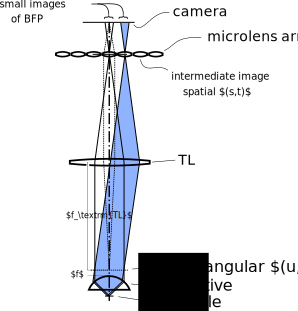
\includegraphics[width=7cm]{microlens-levoy-sketch} %FIXME redraw
  \input{microlens-levoy-sketch.eps_tex}
  \caption{Schematic of microlenses in intermediate image plane (after
    \citep{Levoy2006})}
  \label{fig:microlens-levoy-sketch}
\end{figure}

A microlens array is placed behind the intermediate image plane (see
\figref{fig:microlens-levoy-sketch}). The light that illuminates one
microlens corresponds to one spot in the focal plane of the
sample. The camera is positioned in the focal plane of the microlenses
and captures an image of the back focal plane behind each microlens
(see dashed ray bundle).

The camera captures the four dimensional light field leaving the
specimen with spatial coordinates $(s,t)$ and angular coordinates
$(u,v)$. This data enables computational viewpoint shifting,
refocusing, extended depth of field and aberration correction of the
detected fluorescence emission.


\begin{figure}[!hbt]
  \centering
  \input{microlens-levoy-sketch_2.eps_tex}
  \caption{Construction of an out-of-focus bundle through the light
    field microscope. In order to improve the readability of the
    drawing, the magnification in the microscope was set to $1:1$
    (focal lengths of tube lens and objective are equal). An on-axis
    sample point originating from below the focal plane of the
    objective is imaged into an on axis point between tubelens and
    microlens array. Three of the microlenses reimage the point into
    three points behind the plane of the camera.}
  \label{fig:microlens-levoy-sketch_2}
\end{figure}

\figref{fig:microlens-levoy-sketch_2} shows bundles originating from
an out-of-focus point. Each of the microlenses that are hit by the
circle of confusion reimage a fraction of the of the angular range of
into their images.  This process is crucial because here a lot of the
original image information is lost. The intensities from the
sub-images on the camera can't later be recombined in order to,
e.g. recover a high resolution image of the defocused point
(R.~Heintzmann, personal communication, November 22, 2011).

The light field microscope doesn't utilize the full resolution of
high-NA objectives. This will prevent the use of this technique in its
current form for the detection path of microscopes.

However, the same ideas can be applied in the excitation path. For
illumination purposes lower resolution will often suffice. The light
field technique allows unique control of excitation light intensity
and angles in each point of the sample plane.


{\color{red}
Note that the ray model isn't necessarily sufficient to describe a
light field microscope when the micro lens dimension get close to the
size of the airy pattern of the micro objective. The underlying wave
model can be described by Wigner distributions.

The four dimensional Wigner \todo{don't explain any of the Wigner stuff} distribution $W_U$ of a scalar field
$U(x,y,\tau)$ of narrowband polychromatic light in a plane $z=z_0$ is
defined as the Fourier transform of the mutual intensity $J_U$:
%FIXME is that the spatial coherence function?
\begin{align}
  J_U(x,y,\xi,\eta)&=\left\langle U\left(x+\frac{\xi}{2},y+\frac{\eta}{2},\tau\right) U^*\left(x-\frac{\xi}{2},y-\frac{\eta}{2},\tau\right) \right\rangle_\tau,\\
  W_U(x,y,f_\xi,f_\eta)&=\int\!\!\!\!\int J_U(x,y,\xi,\eta)\ e^{-j2\pi(f_\xi\xi+f_\eta\eta)}\ \textrm{d}\xi\textrm{d}\eta.
\end{align}
In order to express a radiance function it is useful to write the Wigner distribution in its slope-form $W_U^{(\lambda)}$:
\begin{align}
  \label{eq:wigner-slope}
  W_U^{(\lambda)}(x,y,u,v)&:=W_U(x,y,\xi/\lambda,\eta/\lambda),\\
  u&=\xi/\lambda, \quad v=\eta/\lambda.
\end{align}
The observable light field $l^{(T)}(s,t,u,v)$ is obtained by
convolving the Wigner distribution of the scalar field $U$ with the
Wigner distribution the microlens aperture function $T$
\citep{Zhang2009}. 
\begin{align}
  \label{eq:lightfield}
  l^{(T)}(s,t,u,v)
  &=
  W_U^{(\lambda)}(s,t,u,v)\otimes
  W_T^{(\lambda)}(-s,-t,u,v)  
\end{align}
The Fourier uncertainty relates the blur of the $s$ and $u$ directions
\begin{align}
  \label{eq:uncertainty}
  \sigma_s^2\sigma_u^2&\ge\frac{\lambda^2}{16\pi^2}
\end{align}
where the variance $\sigma_x^2$ of a signal $h(x)$ along an axis $x$
represents its ``blur'' and is defined as:
\begin{align}
  \label{eq:variance}
  \sigma_x^2&=\int x^2|h(x)|^2\textrm{d}x.
\end{align}
}

\subsection{Temporal focusing}
\begin{figure}[!hbt]
  \centering
  %\bild{oron} 
  \input{temporal-focus-sketch.eps_tex}
  \caption{Schematic of temporal focusing (after \citep{Oron2005}). A
    grating in the intermediate image plane separates the pulse into
    its spectral components. Out-of-focus areas of the specimen are
    illuminated with a longer pulse. Only the in the focal plane all
    spectral components interfere coherently and form a short
    intensive pulse.}
  \label{fig:oron}
\end{figure}
The axial extent of ultra-short laser pulses can be as thin as a few
microns. A parallel beam can be split into different spectral
components by a grating in the intermediate image plane
\citep{Oron2005}. The tube lens focuses the diffraction pattern into a
line in the back focal plane of the objective.

The objective, which has to be corrected for chromatic aberration and
dispersion, then focuses all the beams into the focal plane. Different
spectral components arrive in the focal plane at the same
time. Out-of-focus points see an extended illumination. For a high NA
objective a pulse duration of $\tau=\unit[20]{fs}$ results in slice of
$z\approx\tau c/2\approx\unit[3]{\mu m}$ thickness around the focus,
where the beam has significant intensity.

Using this technique it is possible to build a widefield two photon
microscope. That only excites fluorophores within the focal plane. The
technique can be further improved by spatially modulating the beam
in the intermediate image plane for CLEM like performance.

\subsection{Phase modulation}
\subsubsection{Digital holography}
\begin{figure}[!hbt]
  \centering
  \includegraphics[height=5cm]{phase-holo} 
  \caption{Schematic of spatial illumination by phase holography
    \todo[inline]{redraw}}
  \label{fig:phase-holo}
\end{figure}
Certain types of liquid crystal spatial light modulators can be used
to modify the phase of light. When such a device is placed into the
back focal plane of a lens, it is possible to control the light
distribution in its front focal plane. An iterative algorithm
(iterative Fourier transform algorithm, IFTA) can be used to establish
a phase image on the liquid crystal display that will result in an
intensity distribution in front of the lens.

\nomenclature{IFTA}{Iterative Fourier transform algorithm}

This approach has been used to excite a two-dimensional pattern in the
specimen \citep{Lutz2008,Zahid2010} and is advantageous especially for
cases where only small parts of the specimen ought to be
illuminated. As opposed to conventional intensity spatial light
modulators the light can be redirected from dark areas into the bright
areas.

% single photon 405nm uncaging, ifta,
% spherical wave approximation
There is also a limited possibility to create three-dimensional
patterns, e.g.\ several points below, in and above the focal plane by
displaying Fresnel zone planes.  For illumination usually a laser with
non-zero interference length is employed. However, this illumination
contains an unwanted ``speckle'' pattern -- noisy non-uniformities. To
a certain extent the contrast of the speckle pattern can be reduced by
controlling spatial and temporal coherence of the illumination
(sweeping the frequency of the laser or changing illumination
direction while the detector is integrating).

Holographic control can be used with two photon excitation as well
\citep{Nikolenko2008} % two photon
but this exacerbates the effect of speckles.
\subsubsection{Generalised phase contrast (GPC)}
\begin{figure}[!hbt]
  \centering
  \includegraphics[width=14cm]{phase} % FIXME redraw
  \caption{schematic of generalized phase contrast \citep{Rodrigo2008}}
  \label{fig:phase}
\end{figure}
A phase contrast microscope objective \todo{modified ?} can be used to
convert a phase image from the intermediate image plane into an
intensity image in the specimen \citep{Rodrigo2008}\todo{read more of
  this}. Compared to digital holography hardly any computation is
necessary. Yet the phase spatial light modulator allows concentrating
a lot of light even into a small region of the specimen as opposed to
other techniques which involve intensity modulation and loose the
light of dark areas.

The generalised phase contrast method is suitable even with spatially
incoherent illumination\todo{slightly ?}.
\subsubsection{Generalised phase contrast and temporal focusing (TF-GPC)}
The combination of generalised phase contrast and temporal focusing
allows selective uniform illumination of in-focus areas
\citep{Papagiakoumou2010}. Usage of a phase spatial light modulator
results in high light efficiency compared to intensity modulation.
Splitting and recombination of the spectral components of the pulse
reduce speckle noise considerably.
\begin{figure}[!hbt]
  \centering
  \includegraphics[width=11cm]{tf-gpc} 
  \caption{Schematic of phase contrast with temporal focusing (TF-GPC)
    from \citep{Papagiakoumou2010}, PCF is a phase contrast filter}
  \label{fig:tf-gpc}
\end{figure}
\nomenclature{PCF}{Phase contrast filter}


\newcommand{\imagw}[3]{
  \begin{figure}[!hbt]
    \centering
    \includegraphics[width=#1]{#2}
    \caption{#3}
    \label{fig:#2}
  \end{figure}
}

\newcommand{\imag}[2]{\imagw{16cm}{#1}{#2}}

\chapter{A prototype for spatio-angular illumination}
\label{sec:setup}
\begin{summary}
  We give a general overview of our spatio-angular illumination
  system. We augment a conventional fluorescence microscope with two
  displays. One is imaged into the back focal plane of the objective
  (for {\bf angular} control) and another display is imaged into the
  sample (for {\bf spatial} control). We explain why we use a gray
  value display for the angular control and why we placed this display
  downstream of the display for spatial control.

  Then we give a more detailed explanation of some if its
  components. Finally we introduce a model that allows to construct
  optimized patterns for spatio-angular illumination.
\end{summary}

\nomenclature{MEMI}{Micro-mirror enhanced micro-imaging. EU FP7
  project reference 215597.}
\section{Overview}
For the EU funded MEMI project it was decided to build a microscope
with two spatial light modulators as depicted in
\figref{fig:memi-simple}. The idea was to image one display (SLM2)
into the sample for spatial control. This gives one way of reducing
unnecessary exposure of the sample (see section \ref{sec:CLEM}).

\begin{figure}[!hbt]
  \centering
  \def\svgscale{1.5}
  \input{memi-simple.eps_tex}
  \caption{Simplified schematic of the MEMI illumination system. A
    homogeneous spatially incoherent light source illuminates from the
    left. It is imaged by $L_1$ and $L_2$ into the intermediate image
    $F'$. Then the tubelens $L_3$ and the objective $L_4$ form an
    image of $F'$ in the sample plane $F$. The first spatial light
    modulator SLM1 is in the plane P', which is conjugate to the pupil
    (BFP) P of the objective. Using SLM1 we can control illumination
    angles in the sample. SLM2 is directly imaged into the sample and
    allows spatial illumination control.} \label{fig:memi-simple}
\end{figure}

An idea we haven't seen implemented so far, is to use another display
(SLM1) for angular illumination control. SLM1 is imaged into the back
focal plane of the objective. We hope to be able to reduce
out-of-focus exposure similar to the ultramicroscopy technique (see
section \ref{sec:light-sheet-microscopy}). However, our microscope
would work with sample in standard slides. We wouldn't need
sophisticated means of holding and rotating the specimen and our
technique could be more easily employed in automatic high-throughput
systems.

\begin{figure}[!hbt]
  \centering
  \def\svgscale{.43}
  \input{hourglass-all.eps_tex}
  \caption{{\bf (a)} Two fluorescent beads are illuminated by all
    angles that an objective can deliver. The sharp image of the
    in-focus bead is deteriorated by blurry fluorescence of the
    out-of-focus bead. {\bf (b)} Angular control allows selective
    illumination of the in-focus bead and results in a better image on
    the camera. {\bf (c)} Angular control is insufficient, when an
    extended in-focus area is illuminated. {\bf (d)} However,
    simultaneous spatial and angular control allows sequential
    excitation of the in-focus beads while excluding the out-of-focus
    bead.}
  \label{fig:hourglass-all}
\end{figure}

Unfortunately, the advantages of easy sample mount and reduced
phototoxicity come at a cost. The difficulty comes from the
illumination control itself. We have two displays that can project two
patterns with approximately $250\times 250$ pixels each. These are a
lot of degrees of freedom.  When we compare this situation to the
other techniques, we see: In ultramicroscopy no sample information is
required. Controlled light exposure microscopy the feedback loop takes
the local in-focus fluorophore concentration point-wise into account.

However, in a spatio-angular microscope, the feedback loop depends on
a lot more data, i.e.\ the full three-dimensional fluorophore
distribution in the specimen. Obviously, if this information was
known, there would be no need for imaging in the first place. For now
let us assume, we know the exact sample, that we want to image --- in
reality, we might only have an estimate of the sample.

In \figref{fig:hourglass-all} we visualize in a simple ray-based
model, how our optical system improves sample
illumination. Fortunately, it turns out that for the most useful
illumination strategies ray optics are sufficient. Nevertheless, some
design decisions require wave optics and we will discuss them on page
\pageref{sec:wave-constraints}.

\figref{fig:hourglass-all}~(a) depicts an illumination configuration,
that resembles the illumination in a confocal microscope. SLM1
transmits everything and the whole back focal plane of the objective
is illuminated. The illumination light is coming from the top.  The
pattern on SLM2 is a single bright spot and illuminates a fluorescent
bead in the focal plane. The incoming cone of light excites the
out-of-focus bead as well. The image on the right of the schematic
shows how an exposure of this scene would look on the camera of a wide
field microscope. The out-of-focus bead gives rise to blurry
background fluorescence light.

By changing the pattern on SLM1 we can limit the light rays, that
would excite the out-of-focus bead. This is indicated in
\figref{fig:hourglass-all}~(b). The camera would only show the image
of the in-focus bead and no background fluorescence from the
out-of-focus bead. Not exciting the out-of-focus bead has several
advantages:
\begin{description}
\item[Less phototoxicity:] Not exciting the out-of-focus areas is
  particularly useful for living biological specimen. Only with
  reduced phototoxicity long term time lapse experiments will show
  subtle biological effects. When imaging stacks the image quality of
  the spatio-angular microscope will surpass wide field microscopes add
  comparable overall dosage.
\item[Less noise:] There is less background light in the camera image,
  leading to a clearer image of the in-focus information. It is
  possible to computationally distinguish and subtract out-of-focus
  light by structured illumination methods but these methods can not
  remove the Poisson distributed photon noise of the out-of-focus
  light.
\item[Precise light control:] In uncaging experiments, a compound is
  added to the medium, that breaks up or releases biologically active
  chemicals, when illuminated. In opto-genetics protein functions,
  e.g.\ an ion pump that can make a nerve cell fire \cite{Nagel2003},
  are controlled by illumination.

  Often a spatially resolved effect (e.g.\ activation of a single
  cell) is required. Until recently 2-photon excitation was the only
  option \citep{Pettit1997,Shoham2005} for such experiments. Only with
  the excitation point spread function of 2-photon microscopes, it is
  possible to limit the excited region to a confined volume with
  sufficiently small $z-$extent.

  Recently a holographic method was published that enables uncaging
  experiments with single-photon excitation \citep{Zahid2010}. It
  allows to sculpt the three-dimensional excitation volume and
  selectively activate groups of cells.

  Similarly our spatio-angular microscope could be
  used\footnote{Presently we have only implemented an optimization
    routine for a sphere model, this is probably not a good model to
    represent neurons.}, to selectively expose target neurons and
  prevent exposure of other cells. The holographic approach can
  achieve a higher light efficiency. However, the method for
  calculating the hologram is very different. In terms of current
  technology, their phase-only display is slower than our intensity
  modulators and potentially we could more easily provide a uniform
  illumination and prevent speckle. At this point it is not obvious
  which approach will be the best.
\end{description}

The two schematics in \figref{fig:hourglass-all}~(a) and (b)
illuminate only one point in the focal plane. One could scan this
point over the whole sample. Then one could computationally
reconstruct a confocal image from the camera images but a tremendous
amount of data would have to be acquired. Therefore, it is useful to
simultaneously illuminate bigger regions in the sample.

However, if these regions are not carefully chosen, angular control
might not work any more. \figref{fig:hourglass-all}~(c) depicts a
sample with two in-focus beads and an out-of-focus bead in between. In
such a situation we would illuminate first one in-focus bead with an
appropriate pattern on SLM1 to prevent exposure of the out-of-focus
bead (\figref{fig:hourglass-all}~(d)) and then the other. 

One drawback of this technique is, that we require prior knowledge
about the fluorophore distribution in the sample, i.e.\ a three
dimensional model of what is going to be imaged.

In three-dimensional time lapse imaging of developing embryos a good
estimate is available when the stacks are acquired with high enough
temporal resolution. Opto-genetics experiments can be designed such,
that the three-dimensional distribution of neurons is known before
single neurons are triggered by light without exposing its neighbours.

For some sample types an estimation of the full three-dimensional
fluorophore concentration within the sample is not practical and might
be unnecessary. Instead, we believe we can project grating images with
the SLM2 and still vary the illumination direction with the mask on
the SLM1. The two camera images with structured illumination could then
be used to recover a sectioned image of the in-focus fluorophore
distribution \citep{2008Lim,Bozinovic2008,2009Santos}. Acquisition of
several such images with different MMA masks would allow to find the
angle with least out-of-focus contributions.


\subsubsection{Wave optical constraints in our spatio-angular microscope}
\label{sec:wave-constraints}
Earlier we claimed, that ray optics are sufficient to find good
patterns for SLM1 and SLM2. Now we will argue with wave optics and we
will see for which patterns the ray model will give wrong
results. Then we discuss the some design decisions in our
spatio-angular microscope.

By design all lenses in \figref{fig:memi-simple} are placed such, that
the back focal plane of one lens is the front focal plane of the
following lens. This simplifies the wave optical treatment of our
system. There is no need for free space propagation. We only have to
propagate the electric field from the front to the back focal plane
for each lens. This is done by a Fourier transform
\citep{Goodman1996}. At the objective $L_4$ we need to be careful. It
needs to be treated differently than standard thin lenses because of
its high aperture. The wave optical simulation is further complicated
by the need to sum over many coherent propagations to properly
represent spatially incoherent light source.  In
Appendix~\ref{sec:sim-angle} we show how to simulate the system using
Fourier optics.

For the current discussion we just note, that the electric fields in
the planes P' and F' in \figref{fig:memi-simple} form a Fourier
transform pair, i.e.\ the electric field illuminating SLM2 is the
Fourier transform of the field transmitted through SLM1. To discuss
this more thoroughly we distinguish the following configurations of
patterns on SLM1 and SLM2:
\newcommand{\sm}[1]{\raisebox{-2.5mm}{\includegraphics{slm-#1}}}
\begin{description}
\item[full SLM1 \sm{full}, point on SLM2 \sm{point}] This
  configuration corresponds to the confocal illumination in
  \figref{fig:hourglass-all}~(a). Angles from the full back focal
  plane will produce a spot in the sample with a size at the
  resolution limit of the objective.
\item[grating on SLM1 \sm{grating-circle}, point SLM2 \sm{point}] The
  grating on SLM1 gives rise to a diffraction pattern on SLM2. If the
  illumination was spatially coherent, there would be at least three
  spots, for $0^\textrm{th}$ and $\pm1^\textrm{st}$ orders. However,
  in our microscope the illumination is spatially incoherent, i.e.\
  each order would have an image of the light source attached to it.
  The small point on the SLM2 only transmits light from the
  $0^\textrm{th}$ order. Therefore, in the back focal would be
  illuminated uniformly and all information of the pattern on SLM1
  would be lost.
  
  For a grating on SLM1 with a big period, the images of the light
  sources overlap and the point on SLM2 would also transmit light from
  the first orders. However, the transmitted from the $+1^\textrm{st}$
  order light comes from a different area of the source than the
  transmitted light from the $-1^\textrm{st}$ order and they will not
  interfere to form an image of the grating in the back focal plane of
  the objective.

  This mode is not useful for illumination. The same intensity
  distribution in the sample can achieved more efficiently by a
  uniform pattern on SLM1.
\item[grating on SLM1 \sm{grating-circle}, full SLM2 \sm{full}]
  Displaying a grating on SLM1 will give rise to a diffraction pattern
  on SLM2. This will result in a bigger illuminated region in the
  sample. This configuration is also not useful and should be avoided.
\item[full SLM1 \sm{full}, grating on SLM2 \sm{grating}] The grating
  on SLM2 will produce a diffraction pattern in the back focal plane
  of the objective with an image of SLM1 attached to each order. Like
  this: \sm{3bigger}. For a very fine grating, the first orders can be
  far apart and only few of the rays can form an image (see also
  Appendix \ref{sec:apotome}).
\item[partial SLM1 \sm{half}, grating on SLM2\sm{grating}] To ensure a
  high contrast of the grating in the sample, it is useful to limit
  the angular range of angles using the pattern on SLM1, so that the
  first orders completely fit\footnote{For a high contrast of a very
    fine grating within the sample the described illumination scheme
    alone is not sufficient. The polarization has to be turned
    according to the grating orientation has well. This could be added
    to our prototype, however it currently not implemented.} through
  the back focal plane of the objective: \sm{3big}.
\item[full SLM1 \sm{full}, full SLM2 \sm{full}] This configuration
  corresponds to a standard wide field microscope. This and similar
  patterns with big convex illuminated areas can be represented with
  good accuracy by a model based on ray optics.
\end{description}

\subsubsection{Discussion of wave optical effects}
From the comparison we see, that our configuration with the second SLM
in the intermediate image F' (\figref{fig:memi-simple}) doesn't allow
high frequency patterns on SLM1. High frequency components of the
image of SLM1 in the back focal plane are heavily influenced by the
pattern on SLM2.

This configuration, which places more importance on SLM2 is a
deliberate design decision.  We chose configuration because we think
it is more important to have high resolution control of the spatial
light distribution in sample space.

One can estimate that with a $63\!\!\times\!\!/1.4$ objective it is
sufficient to illuminate a window with 1\% of the back focal plane
diameter, in order to illuminate an area with $\unit[3]{\mu m}$ in the
sample.  Therefore, as long as the patterns on both SLMs are
sufficiently simple, i.e.\ cover more than a few percent of the full
area, are simply connected and convex, %FIXME simply connected?
the ray-based model is a good representation of the system.

Projecting fine gratings into the sample using SLM2 is possible, but
higher diffraction orders fill more of the back focal plane. Therefore
grating projection will limit the usefulness of angular illumination
control.

The electric fields after SLM1 and on SLM2 form a Fourier transform
pair. Heisenberg's uncertainty relation prevents illumination of a
small spot on SLM2 when SLM1 only transmits very little. It is known,
that a Gaussian transmission function on SLM1 would achieve the
smallest possible spot on SLM1. Therefore, we decided to use a spatial
light modulator, that can display gray values.

\section{Detailed explanation of the optical components}


\begin{figure}[!htbp]
  \centering
  \def\svgscale{2}
  \input{memi-real.eps_tex}
  \caption{Schematic of the light path through our microscope. Laser
    light enters from the lower left, is scrambled and homogenized to
    illuminate the full MMA and LCoS. $F$ is the field plane in the
    sample and its primed versions are conjugated planes. $P$ is the
    pupil of the objective. $B_0$ and $B_1$ are adjustable circular
    apertures. PBS is a polarizing beam splitter. DBS is a dichroitic
    beam splitter.}
  \label{fig:memi-real}
\end{figure}

\begin{figure}[!htbp]
   \centering
   \def\svgscale{2}
   \input{memi-sketch.eps_tex}
   \caption{Schematic of the lenses in the MEMI system and their focal
     lengths. The focal length $f_\textrm{TL}$ of the tube lens can be
     varied. This allows to scale the second intermediate image
     $r''_\textrm{MMA}$ of the micro mirror array to fit the back
     focal plane of different objectives. Dimensions in mm.}
   \label{fig:memi-sketch}
 \end{figure}
 
\imagw{14cm}{setup-photo-blueprint}{The wide field epi-fluorescence
  microscope with attached illumination head. The positions of the two
  spatial light modulators (Micro mirror array (MMA) and liquid
  crystal on silicon display (LCoS)) are indicated. Drawing by Josef
  Wenisch (In-Vision, Austria).}

As opposed to the schematic in the previous section
(\figref{fig:memi-simple}), our spatial light modulators are
reflective.  Also, both displays are not direct intensity modulators.
\figref{fig:memi-real} shows a schematic of the light path in the
combined angular and spatial control system. From now on we call the
first display micro-mirror array (MMA) instead of SLM1 and the second
display liquid crystal on silicon display (LCoS) instead of SLM2.

\paragraph{Illumination.}
A laser light source is scrambled by a rotating micro-lens array and
mixed in an integrating tunnel\footnote{Integration tunnels are used
  to improve the illumination uniformity. Our tunnel has a quadratic
  cross section with \unit[4]{mm} on the side and a length of
  \unit[250]{mm}. Looking into it, one can observe many copies of the
  the entrance. Therefore the light at the tunnel exit comes from many
  directions and forms a uniform profile. The introduction of beam
  homogenization was a quantum step in mass spectroscopy the laser
  ablation process is non-linear and uniform beam profiles allow to
  ablate big areas of the sample with the same condition
  \citetext{priv.\ comm.\ V.\ Deckert}.}.

The distance between the exit of the integration tunnel and the lens
$L_1$ is equal to the focal distance of $L_1$. The MMA is positioned
in the other focal plane of $L_1$. 

\paragraph{Angular control (SLM1).} The micro mirror array
\citep{Berndt2007,Schmidt2010,Berndt2010} consists of $256\times 256$
mirrors with a pitch of \unit[16]{$\mu$m} (see \figref{fig:mma} and
\figref{fig:mma-closeup}). Each mirror hangs on two thin hinges and
can be tilted by up to $2^\circ$ by electrostatic fields. This
corresponds to out-of-plane deflections of $\pm\unit[250]{nm}$.  CMOS
circuits below each mirror allow to maintain a constant tilt for
hundreds of milliseconds. A control board can set new analogue
voltages for each mirror. Loading the full image takes
\unit[850]{$\mu$s}. An accuracy of $\lambda/100$ for the precision of
the actuation is reported \citep{Berndt2011}. Therefore, the MMA is a
programmable phase mask of high efficiency and can achieve frame rates
of up to \unit[1]{kHz} at duty cycles up to \unit[50]{\%}. In a
Fourier filtered configuration it can display gray value images
without the need for time-multiplexing.  An On/Off-contrast from 300
to 800 in the wavelength range from the UV upto NIR can be achieved
\citep{Berndt2011}.

\imagw{14cm}{mma}{{\bf left:} Scanning electron microscope image of
  the micro-mirror array (MMA).  The pixel pitch of the device is
  \unit[0.016]{mm}. The hinges for the tilt movement and the
  electrodes are clearly visible. {\bf middle:} Optical reflective
  microscope image of the MMA. {\bf right:} exaggerated rendering of
  how a 8x8 checker board pattern would be displayed on the
  device. Electron and optical micrograph by Fraunhofer IPMS Dresden
  (Germany)}

\begin{figure}[!hbt]
  \centering
  \includegraphics[width=7cm]{mma-plain}
  \includegraphics[width=7cm]{mma-ill}
  \caption{{\bf left:} Micro mirror array chip during installation of
    the optics. {\bf right:}~Illuminated micro mirror array in the
    aligned system.}
  \label{fig:mma-closeup}
\end{figure}

When all mirrors of the MMA are flat, an image of the tunnel exit $F'''$
is formed in the plane of the aperture $B_1$. The size of the aperture
is chosen to transmit just this image. When mirrors of the MMA are
tilted, they will slightly deflect the light, so that it no longer
passes through the aperture $B_1$. $B_1$ acts as a Fourier filter (or
Schlieren optical system).

If the mirrors of half of the device are deflected to fulfil the blaze
conditions\footnote{This is limited by the maximum tilt angle and
  possible for wavelengths up to \unit[1000]{nm}} then the mirrors
will send all the light into the first order and nothing through the
aperture $B_1$.  The region in the image in $P'$ corresponding to the
tilted mirror will be dark. The mirrors have no significant effect on
the polarization of the light.

\paragraph{Spatial Control (SLM2).}
The lenses $L_2$ and $L_3$ relay the image of the tunnel exit $F'''$
from $F''$ into the plane $F'$ with the LCoS (ForthDD SXGA, pixel
pitch $\unit[13.62]{\mu m}$) \citep{Cartwright2007}. The polarizing
beam splitter ($45^\circ$ wire grid polarizing beam splitter, Moxtek,
UT, US) reflects linearly polarized light towards the LCoS\footnote{In
  order to prevent spurious reflections at the PBS back surface
  (without wire grid coating) and to improve contrast, the incoming
  light should already be polarized}. The electric field vibrates
perpendicular to the paper plane. Depending on the LCoS pixel state
(on or off) an LCoS pixel can rotate the polarization of the returning
light. Light that is polarized in the paper plane is
transmitted\footnote{As it is used in transmission a curvature of the
  PBS doesn't affect the quality of the LCoS image in the sample $F$
  as if the PBS was used in reflection.}  into the illumination tube
lens $\textrm{TL}_\textrm{ill}$ by the PBS (see \figref{fig:lcos} for
a photograph showing tube lens, PBS and LCoS). In order to project a
very fine grating into the sample, the grating lines must be parallel
to the paper plane.

\imagw{5cm}{lcos}{The black cylinder on the left is the variable tube
  lens. Behind this is the polarizing beam splitter and the
  ferroelectric liquid crystal on silicon display.}

The LCoS is of ferroelectric type \citetext{\citealp[see][]{1991Saleh}
  and \citealp[p.~192]{Goodman1996}}.  Its liquid crystals can be
driven very fast between two bi-stable orientations. In order to
prevent a net current, which would eventually destroy the device, its
driver always displays an inverted image after the wanted
one. Therefore it is necessary to modulate the light source
accordingly.


\paragraph{Reimaging of SLM1 into the back focal plane P and SLM2 into
  the sample plane F.}
The lenses $L_3$ and $\textrm{TL}_\textrm{ill}$ relay the Fourier
filtered MMA image from $P'$ into the pupil $P$ of the objective. In
order to accommodate objectives with various back focal plane
diameters, the illumination tube lens is built out of three lens
groups. Its focal length can be varied from \unit[222.8]{mm} up to
\unit[445.4]{mm}, keeping the positions of the focal planes
constant(see \figref{fig:memi-sketch} for a drawing with the focal
length of the other lenses). For this, the lens groups of
$\textrm{TL}_\textrm{ill}$ move such, that the image of the LCoS
behind $\textrm{TL}_\textrm{ill}$ stays in infinity and the MMA (plane
$P''$) is imaged into the pupil $P$, which is \unit[250]{mm} behind
the tube lens. Only the lens groups within the tube lens move,
everything else in the system is fixed. In \figref{fig:tubelens-bfp}
pupil plane $P$ is visible on a translucent plastic card as a screen
\footnote{Later we made an improved screen by melting a drop of wax
  between two coverslips. It gives a better image and fits into the
  objective revolver.} for two different settings of the focal length
of the tube lens.

\begin{figure}[!htbp]
  \centering
  \includegraphics[width=7cm]{bfp1}
  \includegraphics[width=7cm]{bfp2}
  \caption{Images of the micro mirror array in the back focal plane
    with different settings of the variable tube lens. The micro mirror
    array displays the same image (a disk) in both cases.}
  \label{fig:tubelens-bfp}
\end{figure}


\paragraph{Detection.}
Fluorescence light returns from the objective and is reflected by the
dichroitic beam splitter (DBS) through the detection tube lens
$\textrm{TL}_\textrm{det}$ and is imaged on the camera. Note that the
detection works with full efficiency, similar to a standard wide field
fluorescence microscope.


\section{Electronics for synchronization}
Both spatial light modulators can run at most with $50\%$ duty
cycle. Therefore it is necessary to synchronize the displays. Their
controllers allow to upload several hundred frames of image data
before an experiment and keep them in local storage. Images can then
be selected by fast function calls over USB (LCoS) or Ethernet (MMA).

The camera (Clara, Andor PLC, Belfast, Northern Ireland) as the
slowest device is chosen as the master. The camera provides two TTL
outputs. The output ``fire'' is high while the camera is
integrating. The output ``shutter'' goes high \unit[1]{ms} before
``fire'' and provides enough time (\unit[$>850$]{$\mu$s}) for the MMA
controller to tilt and let the mirrors settle.

The LCoS controller can display its images only for certain discrete
times (\unit[20]{ms}, \unit[10]{ms}, \unit[5]{ms}, \unit[200]{$\mu$s})
and it is not straight forward to change this via USB
interface. Therefore we always work with a fixed LCoS display time of
\unit[20]{ms}. The ``fire'' output of the camera also switches the
laser on using an acousto-optic modulator (AOM).

When the z-stage is used, the camera is stopped until the stage has
reached its target position.

\begin{figure}[H]
  \centering
  \input{memi-electronics.eps_tex}
  \caption{The camera triggers both spatial light modulators with its
    TTL outputs. The acousto-optic modulator sends light into the
    system during camera integration.}
  \label{fig:memi-electronics}
\end{figure}

\section{Mapping between the two displays and their respective
  conjugate planes}
\begin{summary}
  It is very important that sample positions, which were obtained by
  analyzing the camera images at specific $z-$stage positions, can be
  fed back to both spatial light modulators. If the mapping between
  sample plane and SLM2 (LCoS) is wrong, then the illumination will be
  wrong. Then the whole illumination concept will break down because
  camera images with the wrong illumination may not show anything.

  The alignment of the SLM1 (MMA) is not as crucial. If the mapping
  between SLM1 and the back focal plane is wrong, the sample will
  still be illuminated just with the wrong angles.
\end{summary}

\subsection{Mapping of the LCoS to the CCD camera}

In order to be able to predict which position on the camera will be
illuminated by a particular pixel of the LCoS a calibration procedure
is run. For this a fluorescent plane is used as a sample. Then single
spots are scanned through a grid of $10\times10$ positions over the
LCoS. The resulting spots on the camera are located and four
parameters defining the rigid transform between camera and LCoS are
estimated (scale, rotation angle, translation in x and y, see
Appendix~\ref{sec:rigid}).

Using these parameters one can then convert between camera and LCoS
coordinates (see \figref{fig:screen_lcos-calib}). Changing the focal
length of the illumination tube lens or a change on the camera position
generally requires a new calibration.

\imagw{7cm}{screen_lcos-calib}{Example of a perfectly fitting rigid
  transform between LCoS and camera. {\bf left:} Mask that is
  displayed on the LCoS. {\bf right:} Camera image of fluorescent
  plane illuminated by mask. The orange lines indicate the borders of
  the original pattern.}

\subsection{Mapping of the MMA to the back focal plane of the
  objective}
First the MMA is aligned to the center of the back focal plane by
displaying an annular ring on the MMA and matching it to the ring of a
phase objective. 

The magnification can be measured by placing a camera on the objective
revolver into the back focal plane. It is also possible to scan a
small window over the MMA while imaging a fluorescent plane as in
\figref{fig:immersion-bfp-scan}. Assuming the image of the MMA isn't
too small, then the periphery of the back focal plane can be located.


\section{Ray-based illumination optimization}
\begin{summary}
  In order to make use of the spatio-angular illumination system it is
  necessary to compute patterns for the two spatial light modulators,
  that will reduce unnecessary illumination in the sample.

  Here we present a simple sphere model that can represent a
  developing embryo. Then we describe a ray-optics based approach to
  finding an optimal circular window to illuminate a target. We then
  improve the optimization algorithm to find more general window
  shapes.
\end{summary}

\subsection{Naive, compute-intensive optimization approach}
When we started the project, we had to decide, how to approach the
illumination optimization. One method is, to simulate the full
spatio-angular microscope with scalar wave optics. Then one can choose
a spatial and an angular pattern and compute the corresponding
intensity distribution in the sample.

Assuming we have a confocal stack of the fluorophore distribution by
measurement or prediction, we can multiply the out-of-focus
fluorophores with the illumination intensity distribution and thereby
estimate a value for the out-of-focus excitation (figure of merrit).

This is one step of the optimization. Now, for the typical
optimization routine, one usually changes one element of the SLM1 and
recompute. The change\footnote{The change is the gradient of the
  figure of merrit in respect to the gray value of the changed pixel.
  For some problems it is possible to calculate the gradients
  analytically. Then the optimizations generally are a lot faster to
  compute. However, if the analytical gradients are available for our
  calculation, they would be similar to \citet{Thurman2009} and quite
  complicated. Therefore we decided to abandon the full simulation.}
of out-of-focus excitation can be used estimate in which direction to
change the gray value of this element, in order decrease out-of-focus
excitation.

Here one step of the optimization --- the computation of the intensity
distribution in the sample depending on the two SLM patterns ---
involves a few tens to hundred three-dimensional Fourier transforms.

A full optimization can quite certainly not be done in a reasonable
time on todays computers.

\subsection{Sphere model}
\label{sec:shadow-map}
One obvious simplification is to not represent the sample as a
three-dimensional grid of measured data.  One useful model are
spheres. In order to represent a \emph{C.~elegans} embryo it is not
necessary to store $300\times 300\times 30$ gray values. Instead one
can just use a few tens of spheres, defined by their center
coordinates and a diameter.

Of course the sphere model is rather crude, e.g.\ it does not describe
the precise shape of a nucleus during division. In the case of a
developing embryo, it is useful to predict one or two minutes into the
future.

\figref{fig:render} shows a model of a \emph{C.~elegans} embryo,
constructed from three-dimensional data of a confocal microscope. The
nuclei are relatively sparse. In order to illuminate one or a few
nuclei we might be able to find a path for the excitation light that
doesn't intersect out-of-focus nuclei --- or at least avoids them. In
our spatio-angular microscope the illumination pattern is represented
by two masks. One for the LCoS and another one for the MMA. In the
following we will construct a ray optics-based algorithm to find such
optimized illumination patterns. For example the red rectangle (with
$\sim\unit[4]{\mu m}$ on the side) would be selected for illumination
with the LCoS. The red cylinder indicates the angle that would be
least obscured by out-of-focus nuclei.

\imagw{6cm}{render}{Rendering of a sphere model, fitted to one time
  frame of a three-dimensional confocal video of a developing
  \emph{C. elegans} embryo (strain AZ212, data provided by Jean-Yves
  Tinevez (Institut Pasteur, Paris) by finding local maxima in the
  difference of Gaussian filtered data \citep{Santella2010}.}

\subsection{Index-matched tracing in illumination direction}
\imagw{12cm}{scan-mosaic_testsample_n100_3_7_5_big_label}{Test case
  for spatio-angular illumination. A target sphere is moved out of a
  layer of spheres. {\bf (a-c)} Rays from the back focal plane are
  traced through the target sphere and the total intersection length
  with out-of-focus spheres is plotted in the diagrams.}

First we assume the beads are embedded in index matched medium. Then
rays only refract at the Gaussian sphere of the objective lens and it
is insignificant how far the target bead is from the interface between
coverslip and medium. Other lenses, such as $\textrm{TL}_\textrm{ill}$
are assumed to be perfect lenses and are not considered here.

Initially we investigated a very simple optimization routine (see
\figref{fig:scan-mosaic_testsample_n100_3_7_5_big_label}). A circular
window with radius $r$ is placed into the back focal plane. Rays from
the centre and periphery of the window are traced through the target
and into out-of-focus spheres. The intersection length of each ray
with each sphere is summed and plotted into a diagram.

\figref{fig:scan-mosaic_testsample_n100_3_7_5_big_label}~a) depicts
the collected values for a point-like window.
\figref{fig:scan-mosaic_testsample_n100_3_7_5_big_label}~b) shows the
same for a window with a diameter of 5\% of the back focal plane. The
left column in the table below the images lists the minimal values
over the full back focal plane. For small windows, a few of the rays
can hit the target without intersecting any other spheres. Increasing
the window size blurs the features in the diagrams.

Here we would choose the window with $r=0.15$
(\figref{fig:scan-mosaic_testsample_n100_3_7_5_big_label}~c)). It
still has a low minimum but the largest amount of light would reach
the target. If we chose a too small value for $r$ we would on the one
hand send only a very small amount of light into the specimen. On the
other hand the field distribution in $P$ is related to the Fourier
transform of the field distribution in $F$ and due to Heisenberg
uncertainty relation a small $r$ in $P$ would illuminate the full
field in $F$.

If we chose a bigger value for $r$ many rays would intersect with
out-of-focus objects.
 
\imagw{12cm}{scan-mosaic_nuc12_n100_3_7_5_big_label}{Raytrace for
  circular window optimization in illumination direction. A window
  with 33\% BFP diameter would be used to illuminate the target
  nucleus.}

\figref{fig:scan-mosaic_nuc12_n100_3_7_5_big_label} shows a similar
raytrace for a sphere model of a \emph{C.~elegans} embryo and chooses
a window size and position which in this sense is optimal.

With the MMA we have a very versatile display and we don't
have to limit ourselves to circular windows. Also the raytraced
optimizations can look noisy when not enough rays are sent through the
sample.
\subsection{Tracing in detection direction}
\label{sec:trace-detect}
For this reason we decided to trace rays from out-of-focus nuclei
through the target into the back focal plane.

\figref{fig:img2-montage_hor}~C) depicts the results of tracing
through a single target point and the out-of-focus spheres in B) in
illumination direction. Note how each out-of-focus spheres result in a
deformed blob in the back focal plane. 

It should be quite clear that the image in
\figref{fig:img2-montage_hor}~D) displays nearly the same information
but was obtained with much less computation.  Here 16 rays were trace
(see Appendix~\ref{sec:sphere-projection}) from the periphery of each
out-of-focus nucleus and one from the centre and the resulting
triangle fan was rasterized into the image. We call this image a
shadow map.


In order for our spatio-angular system to work, neither the MMA, nor
the LCoS should display masks with only a few white pixels. Ray based
simulations are not good models in this case (see
Appendix~\ref{sec:sim-angle} for a description of a wave optical
treatment) and illumination light would simply be impractically low.

For this reason the trace of \figref{fig:img2-montage_hor}~D) is
insufficient. Instead of one target point a sufficiently big area in
the model should be sampled. We sum each of the corresponding shadow
maps into a new one (see the two images on the left in
\figref{fig:bfp2-bfp-images-and-model}. Then we threshold the
accumulated shadow map, so that only the angles with least
out-of-focus targets are illuminated. Finally we blur the mask with a
Gaussian filter in order to prevent ringing of the light distribution
(Gibbs' phenomenon) in sample space.
%FIXME heisst das so?

The diagram on the right of \figref{fig:bfp2-bfp-images-and-model}
displays a sphere model of three-dimensionally distributed beads
($\unit[2]{\mu m}$ diameter, yellow-green, in oil). We obtained this
model with our microscope by displaying several gratings on the LCoS
at full angular illumination and doing a structured illumination
reconstruction (in each pixel the maximum of each pattern minus minimum
of each pattern) of sectioned slices. A matching difference of
Gaussian filter and local maximum search in the three-dimensional
volume gives the centres of the beads.

After constructing the model, the microscope continuously moves the
z-stage onto each bead and illuminates them with their optimized
illumination angles. Bead~26 has been illuminated with very high
angles in order to prevent exposure of the bunch of beads further away
from the objective. Bead~5 is far from any other beads and therefore
more angles can be used for its illumination.


\imagw{14cm}{img2-montage_hor}{{\bf A)} Schematic of the rays between
  back focal plane and sample. {\bf B)} Out-of-focus spheres and the
  target point define a double cone of rays that should not be
  illuminated. {\bf C)} Tracing rays in illumination direction from
  the back focal plane through the sample is an expensive operation
  and results in unnecessarily exact results. {\bf D)} Tracing in
  detection direction from the periphery of out-of-focus spheres
  through a target point into the back focal plane gives nearly
  identical results (shadow map) and is more computationally
  efficient.}

% some raw data with beads in dvi system:
% /mnt/backup/backups-london/mnt/floh/sda3/martin/0226/winterseminar/0216_6
\imagw{10cm}{bfp2-bfp-images-and-model}{{\bf right:} Sphere model of a
  sample with three-dimensionally distributed beads. {\bf left:}
  Optimized MMA masks to illuminate bead 26 or bead 5. The red circles
  indicate the periphery of the BFP of the objective.}



%\imagw{12cm}{structured}{Images of a $\unit[3]{\mu m}$ bead within
%  slightly fluorescent embedding medium under different illumination
%  conditions using a $63\times/1.38$ objective.}




\subsection{Coping with index mismatch of the embedding medium}
So far the described algorithms assumed ideal samples which have been
embedded in a medium with a refractive index, the objective was
designed for.

Biological samples are often embedded in water. However, it might
still be useful, to image with an oil objective. Then the additional
refraction at the glass--water interface has to be taken into account
for spatio-angular illumination.

This makes the task of predicting where to mask the MMA in order to
protect out-of-focus beads more complicated. To circumvent the
spherical aberrations, we have to limit the range of angles, that are
simultaneously illuminating and shift the illumination spot on the
LCoS to correct for the transversal focus shift ($q$ in
\figref{fig:aberration-sketch} right). For this we must have a good
estimate of the distance of the sample from the coverslip--water
interface. See Appendix~\ref{sec:raytrace} for a description of the
raytrace algorithm.

Using an oil immersion objective has the following advantage: By
sending the illumination rays into the sample at a steep angle, close
to the TIRF angle, we can generate a thin sheet of light (see
\figref{fig:hilo}).


\begin{figure}[!hbt]
  \centering
  \def\svgscale{.3}
  \input{screen_0_lines.eps_tex}\qquad
  \input{aberration-sketch.eps_tex}
  \caption{{\bf left:} Rays are starting from periphery of
    out-of-focus nucleus, hitting the target and refracted at the
    water--coverslip interface. {\bf right:} Due to spherical
    aberrations, rays from an on-axis point are shifted to $q(r)$ on
    the camera (where $r$ relates to the angle of the ray in the
    sample). }
  \label{fig:aberration-sketch}
\end{figure}

\begin{figure}[!hbt]
  \centering
  \def\svgscale{.3}
  \input{shift-correction.eps_tex}
  \caption{{\bf top:} A straight ray illuminates a bead embedded in
    oil. {\bf middle:} Embedding the sample in water results in
    refraction of the ray. {\bf bottom:} The refraction can be
    compensated by shifting the target area on the LCoS.}
  \label{fig:shift-correction}
\end{figure}
 
% our reports: they were often corrected by Susan, so i should have a look
% MEMI_WP6_D6_5_Report.pdf     angular clem with grating on lcos
% 6.7    drawing of setup, alignment, sync image, only 11 of the 24 bitplanes
% 6.8a   full field angular control with mma (i used too large images on lcos)
%        rendering of c. elegans embryo, psf calc, ray model,
%        first (yellow) raytraces
% 8.6a   sync image with 11 out of 24

\chapter{Experiments}


\begin{figure}[!hbt]
  \centering
  \includegraphics[width=4cm]{oil}
  \includegraphics[width=4cm]{water}
  \includegraphics[width=4cm]{air}
  \caption{dfaxs}
  \label{fig:immersion-bfp-scan}
\end{figure}

\begin{figure}[!hbt]
  \centering
  \input{tirf-exp.eps_tex} 
  \caption{A fluorescent plane on a slide is embedded in oil, water or
    air. The thickness of the embedding medium is approximately
    $\unit[5]{\mu m}$. The LCoS illuminates a disk with $\unit[30]{\mu
      m}$ diameter while a $14\times 14$ window is scanned over the
    MMA.}
  \label{fig:tirf-exp}
\end{figure}


\chapter{Conclusion}
In this work we, document the development of a spatio-angular
microscope. An important part of the project was to build a working
prototype, which we did in several steps.

Initially, we used a display for spatial control that was connected to
the graphics card. This was sufficient for some proof-of-concept
measurements but there were some problems with triggering. However, we
eventually replaced it with a display having a controller with local
storage. This enables the capturing of image stacks at a sufficient
speed with precise triggering and the light is only sent into the
specimen when a camera exposure is integrated.

However, the preparation time for each stack is quite high.  Uploading
images to the two SLMs is quite slow and somewhat limits the range of
experiments that can be done.

Nevertheless, our microscope prototype provides a different way of
illumination control compared to other approaches in the
literature. In particular, our approach can't control simultaneous
angles in the sample, as seen in the micro-lens based light field
approach \citep{Levoy2009}. That, however, gives our system more
flexibility. While the trade-off between the angular and spatial
resolutions is fixed in the light-field approach, the resolutions can
be easily adapted in our microscope.

The prototype should now be used to investigate the phototoxic effects
biological specimen.





Combine with 2-photon
\appendix
% cascade II /mnt/backup/safe-with-time/torben/safed/y2009/0414
% andor ultra ~/1114  python code for calibration and andor basic for acquisition
\chapter{Read noise characterization in cameras}
\label{sec:ccd-meas}
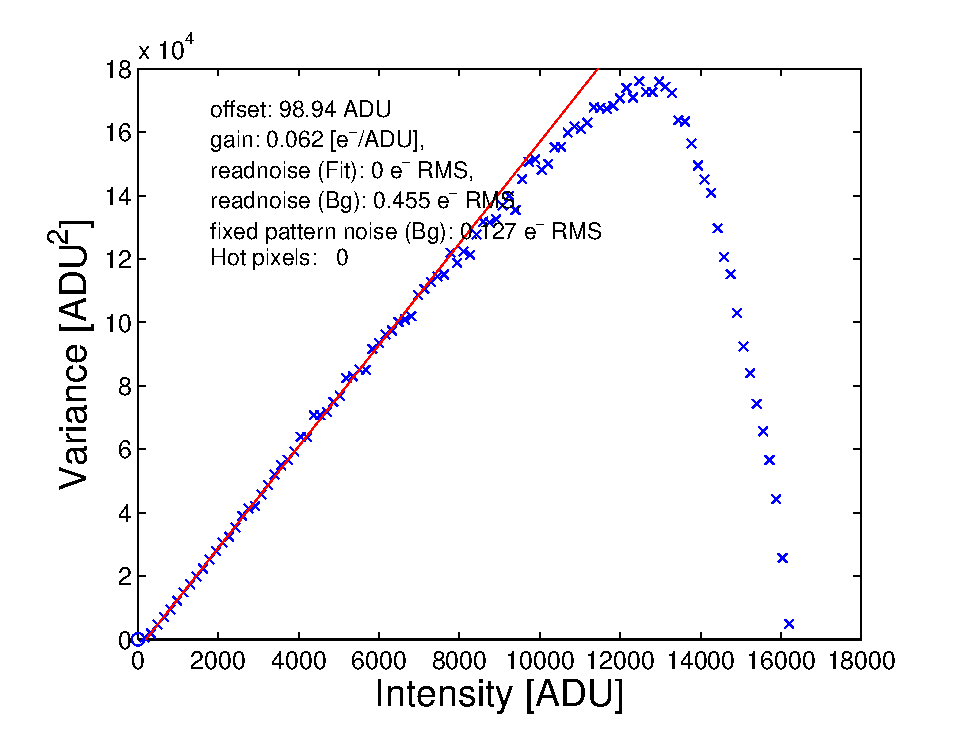
\includegraphics[width=8cm]{../app_cam/andor_emgain100_preamp5_exp30}
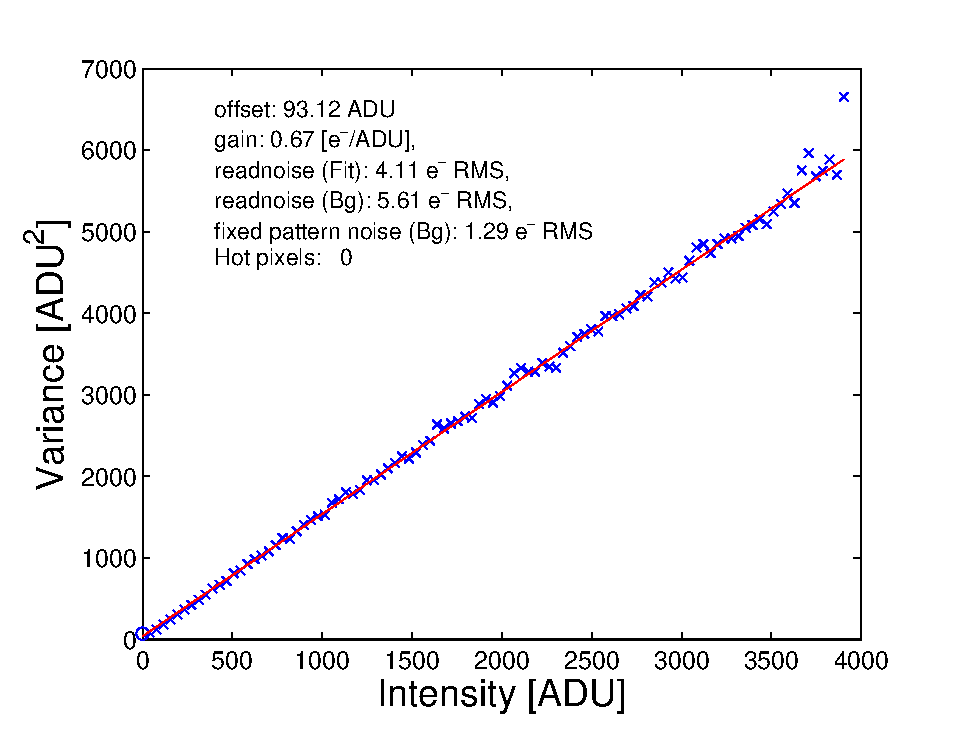
\includegraphics[width=8cm]{../app_cam/andor_normal_preamp5_exp30}
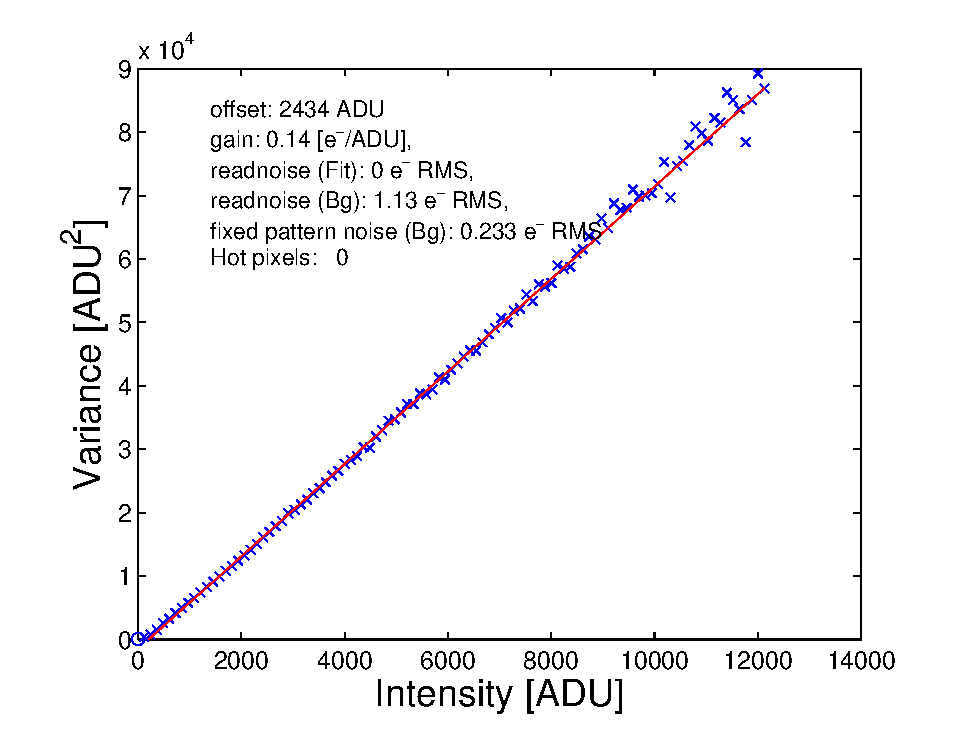
\includegraphics[width=8cm]{../app_cam/cascade_exp400ms_gain3000}
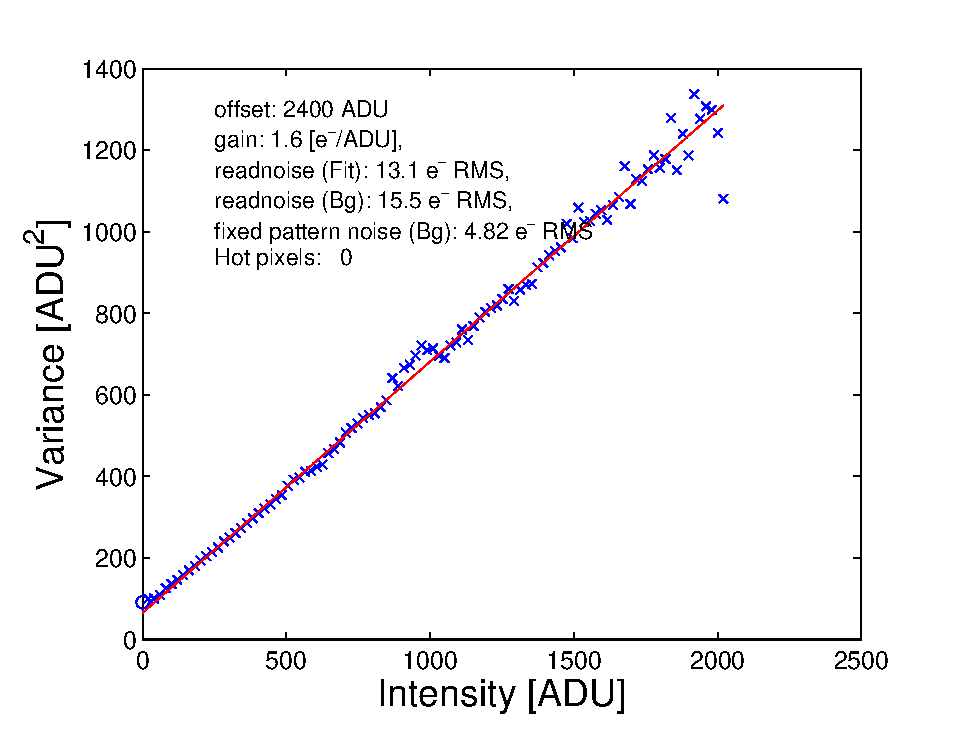
\includegraphics[width=8cm]{../app_cam/cascade_exp400ms_normal}
\includegraphics[width=8cm]{../app_cam/cascade_normal_preamp3_exp30}


\section{Introduction}
In order to characterize the camera we captured sequences of images
that contain a light pattern like this: \includegraphics[width=8cm]{calib-pic}

The images were produced in a fluorescence microscope. The light
source is a DPSS laser with \unit[473]{nm} wavelength. It illuminates
a circular area of the sample. The sample is a fluorescent plane. A
FITC filter cube and a $10\times$ objective were used. The sample was
adjusted to be slightly out of focus in order to obtain a smooth
intensity gradient in the image. For the comparison of the IXon3 with
the newer camera the sample wasn't changed. The Ultra was measured
first. The laser was mechanically blocked while the cameras were
swapped. The following figure depicts the intensity of 20 images that
were illuminated in this way. The relative standard deviation of the
illumination intensity was $0.15\%$.
%\includegraphics[height=7cm]{mean-light}

A sequence (e.g. 20) of such images can be used to determine the
mapping between arbitrary data units (ADU) and the number of detected
photoelectrons. This method is based on the known relation between the
mean number of Poisson distributed photons and its variance.

For the calibration a 2D histogram of the per pixel
variance image and the per pixel mean of the image stack is
plotted. Then the slope of the resulting point cloud is determined.
\section{Calibration of an older IXon3}

%\bbild{ixon_conv1}

In the left diagram of the figures above contains such a 2D
histogram. It was obtained for conventional readout at \unit[3]{MHz}
in our older IXon3 model. The variances are collected in 64 intensity
bins and their averages are plotted as red crosses. The blue line is
the result of a linear fit to the first $60\%$ of the red crosses. Its
slope gives the real gain of the camera that can be used to convert
ADU into photoelectrons (here \unit[1.32]{$e/$ADU}).

The following figures show corresponding measurements using the EM
readout mode with varying EM gain. It is followed by one last
measurement with conventional readout to verify, that the fluorophores
didn't bleach too much during the experiment.

For each figure 20 illuminated images and 20 dark images were
captured. The camera was cooled to \unit[$-75$]{$\,^{\circ}{\rm
    C}$}. The integration time was varied for each gain to have a
maximum of 10000 ADU using a short \unit[10]{ms} acquisition. This was
controlled by an Andor Solis Basic program.

The square root of the mean of the variance of the dark images was
converted into a read noise in electrons per pixel using the real
gain.

The exposure times for the various figures are given in the table that
follows below the figures.

\subsection{Source code for automatic image acquisition}
\begin{verbatim}
function ~GetSaturatingExposure()
        SetKineticNumber(1)
        exp=.01
        SetExposureTime(exp)
        run()
        m=maximum(#0,1,512)
        GetSaturatingExposure=exp*10000/(m-100)
        CloseWindow(#0)
return
name$ = "C:\Users\work\Desktop\martin\20111111\scan-em3\ixon_"
print("start")

SetOutputAmp(1)
print("conv_start")
exp= ~GetSaturatingExposure()
print(exp)
SetExposureTime(exp)
SetKineticNumber(20)
SetShutter(0,1)
run()
save(#0,name$ + "conv1_dark.sif")
ExportTiff(#0, name$ + "conv1_dark.tif", 1, 1, 0, 0)
CloseWindow(#0)
CloseWindow(#1)
        
SetShutter(1,1)
run()
save(#0,name$ + "conv1_bright.sif")
ExportTiff(#0, name$ + "conv1 _bright.tif", 1, 1, 0, 0)
CloseWindow(#0)
CloseWindow(#1)

SetOutputAmp(0)
SetShutter(1,1)
for i = 40 to 300 step 10
        SetGain(i)
        exp=~GetSaturatingExposure()
        print(exp)
        SetExposureTime(exp)
        SetKineticNumber(20)
        SetShutter(0,1)
        run()
        save(#0,name$ + str$(i) + "_dark.sif")
        ExportTiff(#0, name$ + str$(i) + "_dark.tif", 1, 1, 0, 0)
        CloseWindow(#0)
        CloseWindow(#1)
        SetShutter(1,1)
        run()
        save(#0,name$ + str$(i) + "_bright.sif")
        ExportTiff(#0, name$ + str$(i) + "_bright.tif", 1, 1, 0, 0)
        CloseWindow(#0)
        CloseWindow(#1)
next

SetOutputAmp(1)
print("conv_end")
exp= ~GetSaturatingExposure()
print(exp)
SetExposureTime(exp)
SetKineticNumber(20)
SetShutter(0,1)
run()
save(#0,name$ + "conv2_dark.sif")
ExportTiff(#0, name$ + "conv2_dark.tif", 1, 1, 0, 0)
CloseWindow(#0)
CloseWindow(#1)
        
SetShutter(1,1)
run()
save(#0,name$ + "conv2_bright.sif")
ExportTiff(#0, name$ + "conv2 _bright.tif", 1, 1, 0, 0)
CloseWindow(#0)
CloseWindow(#1)
\end{verbatim}

\subsection{Source code for the read noise evaluation}
\begin{verbatim}
#!/usr/bin/env python
# ./ti.py /media/backup/andor-ultra-ixon/martin/20111111/scan-em3/ ultra 2700
import sys
import os

import matplotlib
matplotlib.use('Agg')

from pylab import *
from libtiff import TIFFfile, TIFFimage
from scipy import stats

seterr(divide='ignore')

folder = sys.argv[1]
cam = sys.argv[2]
gain = sys.argv[3]


def readpics(gain,cam='ixon_',isdark=False):
    print 'loading ', os.path.join(folder,cam) + '_' + gain + '_bright.tif'
    fg=TIFFfile(os.path.join(folder,cam) + '_' + gain + '_bright.tif')
    bright,bright_names=fg.get_samples()
    bg=TIFFfile(os.path.join(folder,cam) + '_' + gain + '_dark.tif')    
    dark,dark_names=bg.get_samples()
    return (bright[0],dark[0])

(f,b) = readpics(gain=gain,cam=cam)

bg=mean(b,axis=0)
v=var(f,axis=0)
i=mean(f,axis=0)

ny,nx=64,128
H,y,x=histogram2d(v.flatten(),i.flatten(),bins=[ny,nx],
                  range=[[0,v.max()],[0,i.max()]])
extent = [x[0], x[-1], y[0], y[-1]] 
acc=zeros(x.shape,dtype=float64)
accn=zeros(x.shape,dtype=int64)
s=nx/i.max()
for ii,vv in nditer([i,v]):
    p=round(ii*s)
    acc[p]+=vv
    accn[p]+=1   


fig=figure(figsize=(24, 8),dpi=300)
#subplots_adjust(top=.7,bottom=.2)
hold(False)
title('bal')
subplot(1,3,1)
imshow(log(H), extent=extent,
           aspect='auto', interpolation='none',origin='lower')
hold(True)
ax=x[nonzero(accn)]
ay=acc/accn
ay=ay[nonzero(accn)]
l=round(.6*len(ax))
bx=ax[0:l]
by=ay[0:l]
plot(ax,ay,'r+')
slope,intercept,rval,pval,stderr=stats.linregress(bx,by)
plot(ax,polyval([slope,intercept],ax))
xlabel('intensity/ADU')
ylabel(r'variance/ADU$^2$')
real_gain=1/slope # unit electrons/ADU
read_noise=sqrt(var(b))*real_gain # electrons RMS per pixel
mean_elecs=(mean(f)-mean(b))*real_gain # photoelectrons electrons per pixel
print gain,cam,real_gain,read_noise,mean_elecs,mean(b),rval,pval,stderr
tit='EM-gain: %s, cam: %s, real gain: %.2f e/ADU\n
read noise: %.2f e RMS/pixel, mean: %.2f e/pixel, offset: %.2f'
% (gain,cam,real_gain,read_noise,mean_elecs,mean(b))
title(tit)
subplot(1,3,2)
imshow(var(b,axis=0))
title('variance of darkimages')
colorbar()
subplot(1,3,3)
imshow(mean(b,axis=0))
title('mean of darkimages')
colorbar()
show()
fig.savefig(cam+'_'+gain+'.png')
\end{verbatim}

% ~/from-hp2-notebook/0331/lens
% there is also code
\chapter{Raytracing for spatio-angular microscopy}
\label{sec:raytrace}
\renewcommand{\i}{\nvect i}

Here we give an overview of some useful equations for raytracing
through lens models. The design parameters of our microscope
objectives are not usually known to us. However, this is not an
unsurmountable problem as they can be represented using a simplified
model \citep{Hwang2008}. We use this to simulate the refraction at the
coverslip--medium interface for non-index matched media.

\section{Refraction at plane surface}
We begin by describing refraction at a plane surface\footnote{The
  equations are as in \citep{McClain1993}.}. The wavelength of the
light defines the length of the wave vector $\k_0$. The lengths of the
incident and transmitted wave vectors $\k_1$ and $\k_2$ are given by
the refractive index in their respective half space:
\begin{align}
  k_0&=2\pi/\lambda\\
  k_1&=n_1 k_0\\
  k_2&=n_2 k_0.
\end{align}
The normal $\n$ is directed in the opposite direction of the incident
wave vector $\k_1$. We define the transversal and normal component
vectors:
\begin{align}
  \k_{1n}&=(\k_1\n)\n\\ 
  \k_{1t}&=\k_1 - \k_{1n}.
\end{align}
Both of these components are perpendicular and during refraction the
transversal component of the wave vector is invariant:
\begin{align}
  k_2^2&=k_{2n}^2 + k_{2t}^2\\
  \k_{2t}&=\k_{1t}.
\end{align}
Using the two equations from above we can calculate the length of the
normal component of the transmitted wave vector $\k_2$:
\begin{align}
  k_2^2&=k_{2n}^2 + (\k_1 - \k_{1n})^2\\
  k_{2n}^2&=k_2^2-(\k_1-(\k_1\n)\n)^2\\
  &= k_2^2-(k_1^2-2(\k_1\n)^2+(\k_1\n)^2)\\
  &= k_2^2-k_1^2+(\k_1\n)^2.
\end{align}
Finally we can express the full transmitted wave vector $\k_2$ using
only known quantities:
\begin{align}
  \k_2&=\k_{1t}-\sqrt{k_2^2-k_1^2+(\k_1\n)^2}\n\\
  &=\k_1-(\k_1\n)\n-\sqrt{k_2^2-k_1^2+(\k_1\n)^2}\n.
\end{align}
We divide by $k_2$ with $\k_2/k_2=\t$ and $\k_1/k_2=\eta\,\i$ in order
to introduce unit direction vectors $\i$ and $\t$ for incident and
outgoing light. The relative index change across the interface is
$\eta=n_1/n_2$.
\begin{figure}
  \centering
  \input{refraction.eps_tex}
  \caption{Refraction at an interface transforms the incident wave
    vector $\k_1$ into the outgoing wave vector $\k_2$.}
\end{figure}
\begin{align}
  \t&=\eta\i-\eta(\i\n)\n-\sqrt{1-\eta^2+\eta^2(\i\n)^2}\n\\
  &=\boxed{\eta\i-\left(\eta\i\n+\sqrt{1-\eta^2(1-(\i\n)^2)}\right)\n}
\end{align}
When the radical in the square root is negative a reflection occurs
instead (TIRF). The tangential component is invariant and normal
component inverts the sign:
 \begin{align}
   \k_2&=\k_{1t}-\k_{1n}\\
   &=\k_1 - 2\k_{1n}\\
   &=\k_1-2(\k_1\n)\n\\
   \t&=\boxed{\i-2(\i\n)\n}
 \end{align}
\section{Intersection of a ray and a plane}
Let a ray start at a point $\s$ with direction $\hd$.  A plane
(defined by a point $\c$ and the normal $\n$) intersects this ray if
normal and ray direction are not perpendicular: $\n\,\hd\not=0$. The
distance between the plane and the origin is $h=\c\n$. We can define
the plane equation in Hesse normal form:
\begin{align}
  \r\n=h
\end{align}
We replace the coordinate $\r$ with the ray equation and solve for
the parameter $\tau$:
\begin{align}
  (\s+\tau\hd)\n&=h\\
  \s\n+\tau\hd\n&=h\\
  \tau&=\boxed{\frac{h-\s\n}{\hd\n}}
\end{align}
 \begin{figure}[!hbt]
   \centering
   \input{plane-intersection.eps_tex}
   \caption{Schematic for describing the plane-ray intersection.}
 \end{figure}
\section{Intersection of a ray and a sphere}
Let a ray start at a point $\s$ with direction $\hd$.  Let a sphere
sphere be centered in $\c$ with radius $R$. Their two equations
\begin{align}
  (\r-\c)^2&=R^2\\
  \r&=\s+\tau\hd
\end{align}
define the intersection points. Substitution of $\r$ results in a
quadratic equation for $\tau$:
\begin{align}
  (\s+\tau\hd-\c)^2&=R^2\\
  \l&:=\boxed{\s-\c}\\
  l^2+2\tau\l\hd+\tau^2-R^2&=0\\
  \tau^2+\underbrace{2\l\hd}_b\tau+\underbrace{l^2-R^2}_c&=0
\end{align}
\subsection{Solving the quadratic equation}
If the determinant $d$ is negative the ray misses the sphere and there
is no solution. If the determinant is zero the ray touches the
periphery and there is only one solution. A positive determinant
corresponds to two solutions. In order to prevent numerical errors the following solution should be used \citep{Press1997}: 
\begin{align}
  d&:=\boxed{b^2-4ac}\\
  q&:=\boxed{-\frac{b+\sqrt{d}\sign b}{2}}\\
  \tau&=\boxed{
  \begin{cases}
    \frac{q}{a} &\,\textrm{when}\,\abs{q}\approx 0\\ 
    \frac{c}{q} &\,\textrm{when}\,\abs{a}\approx 0\\
    (\frac{q}{a}, \frac{c}{q}) &\,\textrm{else}
  \end{cases}}
\end{align}
\section{Refraction on paraxial thin lens}
\begin{figure}[!hbt]
  \centering
  \input{lens-fwd.eps_tex}
  \caption{Construction of a ray on a thin lens. The incident beam
    with direction $\i$ hits the lens at the point $\vrho$.}
\end{figure}
The incident beam with direction $\i$ hits the lens at the point
$\vrho$. A line parallel to $\i$ through the center of the lens
defines the point on the focal plane, which will be intersected by the
transmitted ray $\r$ as well.

The triangle $ABC$ is similar to triangle $FOA$. All three angles are
identical because each of the lines are parallel:
$\overline{CB} \parallel \overline{OA} \parallel \vrho$,
$\overline{FA} \parallel \overline{CA}$ and $\overline{AB} \parallel
\overline{OF} \parallel \i$. The side $\overline{OF}$ is hypothenuse
of a right angled triangle. Its ancathete with respect to the angle
$\theta$ has length $f$. Therefor the we can deduce the length
$\abs{\overline{OF}}=f/\cos\theta$.

Between the two similar triangles, the following relation holds and
can be used to calculate the length $\abs{\overline{BC}}$:
\begin{align}
  \frac{\abs{\overline{BC}}}{\abs{\overline{BA}}}&=
  \frac{\abs{\overline{OA}}}{\abs{\overline{OF}}}\\
  \frac{\abs{\overline{CB}}}{1}&=
  \frac{\rho}{f/\cos(\theta)}.
\end{align}
Given its length, the vector $\overline{CB}$ can now calculated,
because we know its direction to be along $\vrho$. With this vector
and $\i$ we can now obtain the (arbitrarily scaled) transmitted vector
$\r'$. We could normalize it but it turns out to be useful for the
high NA immersion lens to find the vector $\r$, that ends in the focal
plane.  The procedure from above is condensed in the following
equations:
\begin{align}
  \vrho&=(x_0,y_0,0)^T=\rho (\cos\phi,\sin\phi,0)^T\\
  \phi&=\arctan(y_0/x_0)\\
  \cos\theta&=\boxed{\i\hz}\\
  \r'&=\i- \frac{\cos\theta}{f}\vrho\\
  \r&=\boxed{\frac{f}{\cos\theta} \i -\vrho}
\end{align}

\section{Refraction through oil objective (illumination)}
\begin{figure}[!hbt]
  \centering
  \input{obj-fwd.eps_tex}
  \caption{Construction of a ray on an high numerical aperture oil
    immersion objective. As opposed to a thin air lens the objective's
    focal length needs to be corrected by the focus difference vector
    $\a$ to accommodate for the immersion and we must take into
    account spherical principal surface.}
\end{figure}
It is possible to augment the results of the calculation from the
previous chapter to treat an aplanatic immersion objective
\citep{Hwang2008}.

We account for the immersion medium by shifting the focal plane in
sample space to $nf$ using the focus difference vector $\a$.
\begin{align}
  \a &= \boxed{f (n-1) \hz} \\
  R &= \boxed{nf}
\end{align}
The principal surface\footnote{An image forming system focusses
  parallel light into a point. Its prinicipal surface is the surface
  where an incident parallel ray intersects with a line along the
  transmitted image forming ray.} is a sphere of radius $R=nf$ around
the image point (\cite{Smith2000} p.~22). In the paper
\citep{Hwang2008} they express the deviation between the real
principal surface and the principal plane with an approximation for
small angles $\theta$ and $\phi$:
\begin{align}
  \s &= \boxed{(R - \sqrt{R^2-\rho^2})\i}
\end{align}
This is an approximation because it only takes into account the
perpendicular (along $\z$) distance between plane and sphere. They
demonstrate the viability of this approximation by comparing its
results with a full raytrace through a $100\times\,1.41$
objective. Focus displacement errors are less than \unit[130]{nm} for
a field of $\unit[86.4]{\mu m}$ radius. This is sufficient for our
problem. As we anyway have the code for a ray--sphere intersection, we
can use it here as well and calculate an exact vector $\s$.

The final ray exiting the objective has the direction $\r_0$:
\begin{align}
  \r_0 &= \boxed{\r + \a - \s}.
\end{align}
\section{Reverse path through oil objective (detection)}
Now we consider the oil objective in the reverse direction (see
\figref{fig:obj-ref-full}). We have a ray starting within the sample
and want to know the transmitted ray in the pupil.

\subsection{Easy case: back focal plane positions only}
If we are only interested in positions of rays in the back focal
plane, we don't have to do full raytracing. If we are imaging beads in
index matched embedding medium and we want to calculate shadow maps
for the MMA (see section \ref{sec:shadow-map}), we don't need a full
raytrace. Instead it is sufficient to ignore ray origins and just
consider their directions.

A unit ray direction $\i=(x,y,z)^T$ in sample space is transformed
into a position $\r_b=(x',y')^T$ in the back focal plane of the
objective. The azimuthal angle $\phi$ isn't changed when going through
the objective. The polar angle $\theta$ defines how far off axis the
back focal plane is hit.
\begin{align}
  \phi'&=\phi=\arctan(y/x)\\
  \theta&=\arcsin(\sqrt{x'^2+y'^2})\\
  r_b&=nf\sin\theta\\
  \r_b&=r_b(\cos\phi',\sin\phi')^T
\end{align}
 \begin{figure}[!hbt]
   \centering
   \input{obj-rev.eps_tex}
   \caption{Schematic for tracing a ray direction $\i$ from sample
     space into the back focal plane. The bigger the angle between
     $\i$ and the optical axis, the further outside the ray will pass
     through the back focal plane.}
 \end{figure}
\subsection{Full raytrace}
If we are also interested in the angles of the transmitted rays in the
back focal plane, when we want to trace the rays further into the
camera or if we want to consider aberrations due to an index mismatch
of the embedding medium, we will have to calculate a full raytrace, as
describted below.

The position of the objective is defined by its principal point $\c$
and the normal $\n$ (directed along optical axis towards sample
space). The incident ray is defined by its starting point $\p$ and the
direction $\i$. First we calculate the center of the gaussian sphere
$\vect g$:
\begin{align}
  \vect g &= \c + nf \n.
\end{align}
Then we obtain the position $\p'$ by intersecting the incident ray and
the plane perpendicular to the optical axis through $\vect{g}$.  The focus
difference vector is defined by its length and the optical axis. It
can be used to calculate an intermediate point $\p''$.
\begin{align}
  \a &= -f(n-1)\n \\
  \p'' &= \p' + a.
\end{align}
The point $\p''$ has now been shifted, so that a thin air lens would
image it exactly as the oil objective would image $\p'$. We can use
$\p''$ to find the direction $\t$ of the transmitted ray. It is just
the normalized difference vector $\vect m$ to the principal point.
\begin{align}
  \vect m &= \c - \p'' \\
  \t &= \vect m / \abs{\vect m}.
\end{align}
As a last step we calculate the starting point $\e$ of the transmitted
ray by intersecting the incident ray with the gaussian sphere.
\begin{figure}[!hbt]
  \centering
  \input{obj-rev-full.eps_tex}
  \caption{Construction to find the transmitted ray through an oil
    immersion objective from a point within the sample.}
  \label{fig:obj-ref-full}
\end{figure}
\subsection{Treatment of aberration (detection)}
Now we consider a ray originating in point $\p$ with direction $\i$
within an immersion of index $n_e$. We want to treat the problem of a
non-matched embedding medium $n_e\not=n$. We find the intersection
$\f$ of the ray with the coverslip--embedding interface and refract to
obtain $\i'$. We calculate the time $t$ a photon takes, to travel from
$\p$ to the interface $\p$:
\begin{align}
  t = \abs{\f - \p} n_e c
\end{align}
and extend the path of the photon backward along $\i'$ by
$t/(cn)$. This results in the corrected position $\p'$ that indicates
where the photon would have originated if the embedding would have
been index matched.  Now we can apply the equations from the previous
sections on the ray defined by $\p'$ and $\i'$ to obtain the
transmitted ray in the pupil.

 \begin{figure}[!hbt]
   \centering
   \input{obj-rev-full-emb.eps_tex}
   \caption{Construction that treats the interface between embedding
     and immersion medium}
 \end{figure}
\section{Sphere projection}
When we model our sample as a collection of spheres, it is useful to
trace rays from the periphery of these spheres through an in focus
target $\c$ into the back focal plane. Here we construct the rays.

The tangents of an out of focus sphere $S^\s_r$ centered at $\s$ with
radius $r$ that pass through the target $\c$ form a double cone
(assuming $\c$ is outside of $S^\s_r$. The tangents touch the surface
of the sphere $S^\s_r$ at the circular intersection $C$ with the sphere
$S^\c_R$ centered at $\c$ with radius $R=\abs{\c-\s}$. Radius $R$ is
the distance from the target to the center of the out of focus sphere.
\begin{figure}[!hbt]
  \centering
  \input{touch-cone.eps_tex}
  \caption{Schematic of how an out of focus nucleus defines a cone of
    tangential rays.}
\end{figure}
In order to find a point $\e$ where a tangent touches the out of focus
sphere, it is sufficient to solve the following equation in a 2D
coordinate system with the origin in the center $\s$ of the out of
focus sphere:
\begin{align}
  (x-R)^2+y^2&=R^2\\
  x^2+y^2=r^2
\end{align}
There are two solutions:
\begin{align}
  x_1&=\frac{r^2}{2R}\label{eqn:x1}\\ 
  y_{1/2}&=\pm\frac{r}{2R}\sqrt{4R^2-r^2} \label{eqn:y1}
\end{align}
In the case $R<r$ the out of focus nucleus is intersecting the target,
obliviating the reason to do the projection in the first place.

We construct two vectors $\hx$ and $\hy$ in order to transform the
solution from 2D into 3D. The (unnormalized) direction $\x$ of the
x-axis of this coordinate system is given by the difference vector of
the target $\c$ and the nucleus center $\s$. The direction $\y$ must
be perpendicular to $\x$ and is obtained by calculating the cross
product with another vector $\q$.  We ensure that $\q$ and $\x$ are
not colinear. The vectors $\q$ and $\x$ are colinear, when the
absolute value of their scalar product equals the square of the length
$\abs{\q\x}=\x^2$.
\begin{align}
  \x&=\c-\s\\
  \q&=\begin{cases}
    (0,0,1)^T & \textrm{when}\ \abs{x_z}<\frac{2}{3}\abs{\x}\\
    (0,1,0)^T & \textrm{else}
  \end{cases}\\
  \y&=\x\times\q \\
  \hx&=\x/\abs{\x}\\
  \hy&=\y/\abs{\y}
\end{align}
Now we can sample the intersection circle $C$ in order to create
viable starting points $\e$ for tangential rays.  Let $R_\phi^\hc$ be
a rotation matrix that rotates a vector by angle $\phi$ around an axis
$\hc$. A point $\e$ on the circle is then defined using one solution
from equations \ref{eqn:x1} and \ref{eqn:y1}. The ray direction $\f$
is then easily obtained:
\begin{align}
  \e&=\s+x_1\hx+y_1R_\phi^\hx\hy\\
  \f&=\c-\e.
\end{align}
Tracing a sufficient number of rays (e.g.\ 16) with direction $\f$ for
different angles $\phi$ to the back focal plane gives the projection
of the intersection circle $C$. Note that this projection in general
is not a circle anymore.

For practical reasons its useful to project vector $\x$ as well. It
can be used as the center of the (distorted) shape on the back focal
plane to rasterize it as a fan of triangles.

%FIXME maybe compare to ./cyberpower-store/0314/zeiss-patents/20080106795-correction-ring.pdf 
%or US7268953-63x.pdf



% 0609/scan
\chapter{Mapping of camera coordinates onto LCoS coordinates}
\label{sec:rigid}
\begin{summary}
  In our microscope the plane of the camera is conjugate to the plane
  of the LCoS display. It is useful and for most illumination
  strategies crucial to be able to relate a camera position back to
  the LCoS. Then the information from one exposure can be used to
  control the illumination in the next.

  Whenever the camera is moved or the variable tubelens is changed, we
  have to recalibrate the system with a fluorescent plane sample on
  which we project single spots with known positions on the LCoS. Here
  we describe a robust approach to find a rigid transform between LCoS
  and camera coordinates.
\end{summary}
\section{Description of the rigid transform}
In order to relate coordinates on the LCoS display with pixel
positions on the camera, we found it suffices to use a rigid
transform. The rigid transform between display and camera is defined
as:
\begin{align}
  \r^d&=s \textrm{R}_\phi \r^c + \vect t\\
  \textrm{R}_\theta&=\begin{pmatrix}
  \cos\phi & q\sin\phi \\
  -\sin\phi & q\cos\phi \\ 
  \end{pmatrix}
\end{align}
where $\r^d$ is a point on the display, $\r^c$ is a point on the
camera and $q$ can be either $+1$ or $-1$. The value of $q$ is $-1$,
if there is a single axis reflection. It is $+1$ if there is no
reflection.

\begin{figure}[!hbt]
  \centering
  \input{calib-align.eps_tex}
  \caption{Given $n\ge 4$ camera images of a display showing one
    point.  It is possible to calculate the parameters of the rigid
    transform parameters scaling $s$, rotation angle $\phi$,
    translation vector $\vect t$.}
  \label{fig:calib-align}
\end{figure}



One can find the transform parameters scaling $s$, rotation angle
$\phi$, translation vector $\vect t$ by minimizing
\begin{align}
  \sum_i^n \abs{s \textrm{R}_\phi \r^c_i+\vect t -\r^d_i}^2 \label{eq:rigid-sum}
\end{align}
for all $n$ points on the display $\r^d_i$ and there corresponding
camera positions $\r^c_i$.  Each term of the sum can be expressed as
two scalar terms:
\begin{align*}
  \sum_i^n&
  \abs{s(\cos\phi r^c_{ix}+q\sin\phi r^c_{iy})+t_x-r^d_{ix}}^2
  +
  \abs{s(-\sin\phi r^c_{ix}+q\cos\phi r^c_{iy})+t_y-r^d_{iy}}^2
\end{align*}

The following Maxima code will find the solution to the least squares
problem:
\begin{verbatim}
load(minpack)$
q:-1;
g(s,p,tx,ty):=[s*( cos(p)*<cx>+q*sin(p)*<cy>)+tx-<dx>,
               s*(-sin(p)*<cx>+q*cos(p)*<cy>)+ty-<dy>, ... ]$
minpack_lsquares(g(s,p,tx,ty), [s,p,tx,ty], [0.88,-3.1,1200,-20]);
\end{verbatim}
We define the function \verb!g! to contain all the terms of the sum.
This can easily written by a program that constructs the lines
according to the given pattern, replacing \verb!<cx>!, \verb!<cy>!
with camera coordinates and \verb!<dx>!, \verb!<dy>! with display
coordinates.

The function \verb!minpack_lsquares! calls the subroutine \verb!lmder!
which was originally developed for the Fortran\footnote{Rather than
  calling a Fortran library Maxima calls a version of this function
  that was automatically translated into Common Lisp via {\sf f2cl}.}
package \verb!minpack!.

{\small
\begin{verbatim}
c     subroutine lmder (http://www.netlib.org/minpack/lmder.f)
c     the purpose of lmder is to minimize the sum of the squares of
c     m nonlinear functions in n variables by a modification of
c     the levenberg-marquardt algorithm. the user must provide a
c     subroutine which calculates the functions and the jacobian.
c     the subroutine statement is
c       subroutine lmder(fcn,m,n,x,fvec,fjac,ldfjac,ftol,xtol,gtol,
c                        maxfev,diag,mode,factor,nprint,info,nfev,
c                        njev,ipvt,qtf,wa1,wa2,wa3,wa4)
\end{verbatim}
}

\noindent The reason for using Maxima is, that it calculates the symbolic
Jacobian for the problem. This makes it straight forward to change the
simple rigid transform to a model with more parameters.

The following Common Lisp code shows how the result of the
optimization can be used to initialize the OpenGL modelview matrix to
transform objects in its buffer, so that they will appear at the given
positions on the camera.

{\small
\begin{verbatim}
(defun load-cam-to-lcos-matrix (&optional (x 0s0) (y 0s0))
  (let* ((s 0.828333873909549) (sx  s)        (sy  (- s))
         (phi -3.102)          (sp (sin phi)) (cp (cos phi))
         (tx 608.433)          (ty 168.918)
         (a (make-array (list 4 4) :element-type 'single-float
             :initial-contents
             (list (list (* sx cp)    (* sy sp)  .0   (+ x tx))
                   (list (* -1 sx sp) (* sy cp)  .0   (+ y ty))
                   (list .0           .0        1.0   .0)
                   (list .0           .0         .0  1.0)))))
    (gl:load-transpose-matrix (sb-ext:array-storage-vector a))))    
\end{verbatim}
}
  

\noindent
Alternatively, here is the equivalent code in C:

{\small
\begin{verbatim}
float m[4*4]; // OpenGL Modelview Matrix
float s=-.8749328910202312,
      sx=s,sy=-s,phi=-.8052030670943575,
      cp=cos(phi),sp=sin(phi),
      tx=1456.71806436377,
      ty=910.4787738693659;
  m[0]=   sx*cp;   m[4]=sy*sp;   m[8] =0;    m[12]=tx; 
  m[1]=-1*sx*sp;   m[5]=sy*cp;   m[9] =0;    m[13]=ty; 
  m[2]=0;          m[6]=0.;      m[10]=1;    m[14]=0;  
  m[3]=0;          m[7]=0.;      m[11]=0;    m[15]=1;  
glMatrixMode(GL_MODELVIEW);
glLoadMatrixf(m);
\end{verbatim}
}
\section{Experimental example and image processing}

For the calibration a fluorescent plane (see
\figref{fig:rigid-pics}~left for a uniform wide field image) is imaged
with the LCoS display showing spots in the illuminated area.  Ideally
for this measurement all mirrors on the MMA are undeflected and the
apertures $B_0$ and $B_1$ completely open (see
\figref{fig:memi-real}). Then the square exit of the integrating
tunnel illuminates the biggest possible area on the LCoS.

\begin{figure}[!hbt]
  \centering
  \includegraphics[width=7cm]{o102}
  \includegraphics[width=7cm]{o035}
  \caption{{\bf left:} Uniformly illuminated fluorescent plane (mono
    and double layer of yellow beads with \unit[110]{nm} diameter,
    excited with \unit[473]{nm} laser in a 63x/1.47 objective). {\bf
      right:} Image with the the LCoS displaying a disk with 24 pixels
    diameter (corresponding to $\unit[2.4]{\mu m}$ in the sample)
    centred at LCoS position $(550,750)$.}
  \label{fig:rigid-pics}
\end{figure}

% i believe the TL_ill is set to r_MMA=3.84mm in BFP 
% f_TLill = 352 mm
% mag_real = mag / f_zeiss * f_TLill 
% pixel-pitch-lcos / mag_real
% one pixel is: 13.62 / 63 * 164.5 / 352 = 101nm

\begin{figure}[!hbt]
  \centering
  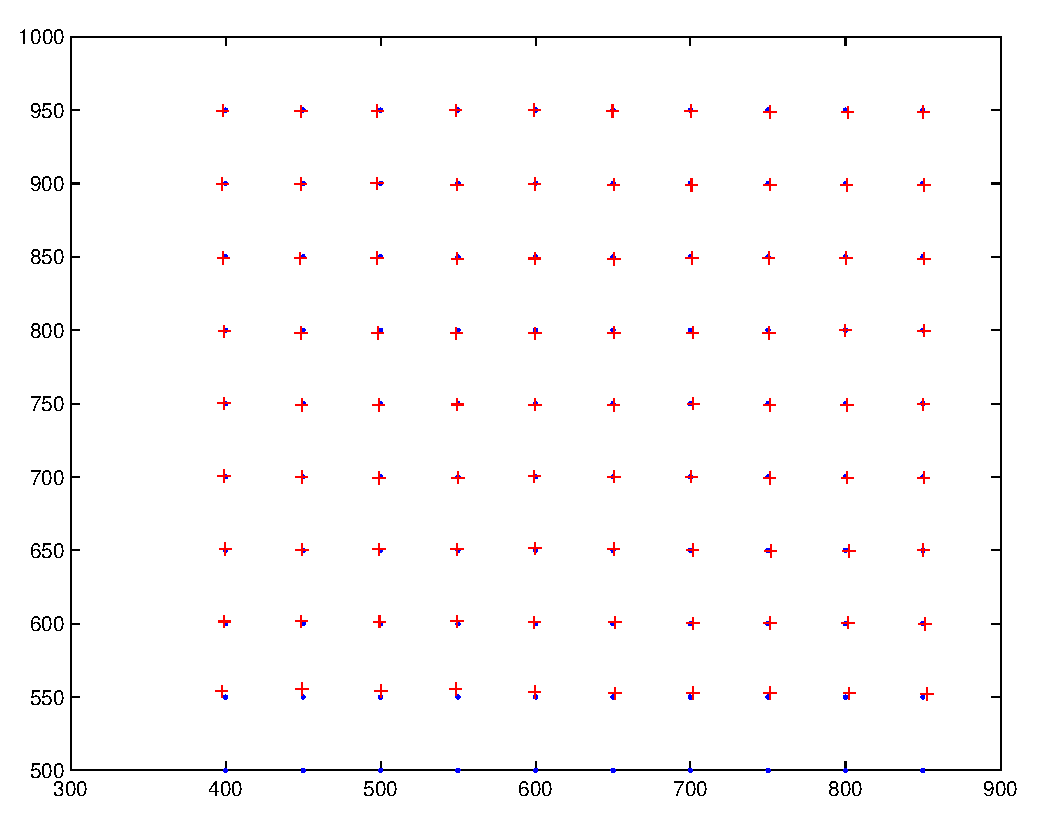
\includegraphics[width=12cm]{../rigid/rigid-compare}
  \caption{Red ``$+$'' signs indicate where the spots that were
    localized in the camera images end up after a rigid
    transform. There is sufficient agreement with the original
    display positions.}
  \label{fig:rigid-compare}
\end{figure}

For the calibration $10\times10$ images (100 images, each containing
one bright spot at a different position) were captured with a disk of
24 pixels diameter at the positions $(400+50i,500+50j)\ \forall i,j\in
[0,99]$. Furthermore, one uniformly illuminated image is used to
correct for intensity fluctuations in the fluorescent plane.  The
following Matlab/DIPimage code is used to normalize the images and
localize the spots. The coordinates are then assembled into the Maxima
command that finds the parameters of the rigid transform. Finally the
transformed spot positions from the camera images are compared with
the original LCoS pixel positions.

The following Matlab listing shows how to open the image files:
% cd /mnt/scan 
{\small
\begin{verbatim}
%% load the files
% 0 .. 99 spot images
% only 10..99 usable because the first are on border and not illuminated
a = newim(1392,1040,103);
for i=0:102
    % Andor's FITS format isn't read correctly
    % correct this by adding 2^15
    a(:,:,i) = 2^15 + readim(sprintf('o%03d.fits',i));
end
\end{verbatim}}

  Of the 103 images, that are loaded into \verb!a!, the first 100
  contain spots and the image at the zero-based index 102 is the
  uniformly illuminated image shown in \figref{fig:rigid-pics} left.
  The other two images at indices 100 and 101 are two centered disks
  with different diameters and are not used here.

{\small
\begin{verbatim}
bright = squeeze(a(:,:,102));  % histogram of uniformly illuminated
                               % image has minimum at 800 ADU
mask = gaussf(bright,8) > 800; % create mask with illuminated area
bg = 510;                      % the background is be 510 ADU

posmax = newim(100,2);
for i = 10:99
    % correct for sample non-uniformity 
    corr = (squeeze(a(:,:,i)) - bg) / bright * mask;
    % find coordinates of maximum
    [coords,vals]=findmaxima(gaussf(corr,32));
    [valss,valsind] = sort(vals);   % sort coordinates by intensity
    tmp = coords(valsind,:);        % collect the maximum with highest
    posmax(i,:) = tmp(end,:);       % intensity into result
end
\end{verbatim}}
  
  The DIPimage toolbox provides the function \verb!findmaxima!, that
  locates all local maxima in an image with subpixel accurac y. We
  sort the result by gray value and only use the biggest.  The
  measured 100 camera coordinate pairs in \verb!posmax! correspond to
  $\r^c_i$ in equation \ref{eq:rigid-sum}.
 
  From Matlab we create the file \verb!fit.max! with batch commands
  for Maxima. Then we run Maxima. When it is finished after a few
  seconds, the file \verb!max.out! will contain the four fitted
  parameters.
 
{\small
\begin{verbatim}
c = double(posmax)';
cmd = '';                       % collect equations in maxima format
for i=10:99
    dx = num2str(400+50*mod(i,10));
    dy = num2str(500+50*floor(i./10));
    cx = num2str(c(i+1,1)); 
    cy = num2str(c(i+1,2));
    cmd=[cmd ' s*( cos(p)*' cx '+q*sin(p)*' cy ')+tx-' dx ', ...
         s*(-sin(p)*'cx '+q*cos(p)*' cy ')+ty-' dy ','];
end
cmd(:,end) = []; % delete last comma

% load the fitting package and start defining the merit function g
pre = 'load(minpack)$ q:-1; g(s,p,tx,ty):=[';
% now put cmd between
% call the fitting function and store the parameters into max.out
cod = [']$ fit:minpack_lsquares(g(s,p,x,y),[s,p,x,y],[.88,-1.3,1200,-20]);' ...
 'write_data(fit[1],"max.out");']

fid = fopen('fit.max','w'); % write maxima commands into file 
fwrite(fid,[pre cmd cod]);
fclose(fid);
[max_status,max_result]=system('maxima -b fit.max');  % execute maxima
\end{verbatim}}

  We load the transformation parameters back into Matlab and create
  the diagram \figref{fig:rigid-compare} to visualize, how well the
  transform matches camera and display coordinates.

{\small
\begin{verbatim}
% load rigid transformation parameters from the file into matlab
params = load('max.out')'; 
scale = params(1); phi = params(2);
tx = params(3);    ty = params(4);

mirr = -1;
R = [cos(phi),mirr*sin(phi);
     -sin(phi),mirr*cos(phi)];
T = [tx ty]';

%% plot the two grids on top of each other
mapped = zeros(100,2);
for i=11:100 % camera coordinates into display coordinates
    mapped(i,:) = (scale*R*q(i,:)'+T)';
end

dpos = zeros(100,2);
for i=0:99 % calculate display points
    dpos(i+1,1) = 400+50*mod(i,10);
    dpos(i+1,2) = 500+50*floor(i./10);
end

hold off;  plot(dpos(:,1),dpos(:,2),'.');
hold on;   plot(mapped(11:end,1),mapped(11:end,2),'r+');
\end{verbatim}}
% print -depsc2 /home/martin/thesis/kielhorn/rigid/rigid-compare

\section{Conclusion}
The rigid transform and our method to estimate its parameters is a
sufficient and robust method, to map the coordinates of our camera
into those of the spatial display.

The rigid transform can be done directly in OpenGL. Hence, it is
trivial to render a properly transformed texture of the camera
image which is then shown on the display.

An advantage over other methods, e.g. finding a homology matrix via
RANSAC, is that the result is not a transformation matrix but
separated parameters for scaling, rotation and translation. 
\include{app_hilo}
\chapter{Wave optical simulation of the spatio-angular microscope}
\label{sec:sim-angle}

\begin{figure}[!hbt]
  \centering
  \def\svgscale{1.5}
  \input{memi-simple.eps_tex}
  \caption{Given two masks for MMA and LCoS plane, it is possible to
    predict the light intensity in the sample by propagating fields
    from each MMA pixel into sample space and integrating an
    incoherent sum there.}
  \label{fig:memi-simple-app}
\end{figure}

The objective of an optical microscope is defined by its support on
the Ewald sphere, i.e. the set of angles at which $k-$vectors
contribute to the image. In the following we assume an ideal air
objective with unit numerical aperture. This objective collects all
light emitted into one half space and therefor half the Ewald sphere.

The following code calculates the amplitude point spread function of
such an objective (see \figref{fig:simple-apsf}~right for a display of its
$x-z$~section).

{\small
\begin{verbatim}
n = 128;
nh = n/2;

% generate spherical shell in k-space
a = sinc(rr(n,n,n));
ka = ift(a);

% select top of the shell (NA=n):
ke = ka * (zz(ka)<0);

% show kx-kz section of ewald-sphere
ke(:,nh,:)

e = ift(ke);

% xz section of electric field
e(:,nh,:)
\end{verbatim}
% writeim(255/max(abs(ke(:,nh,:)))*abs(squeeze(ke(:,nh,:))),'/home/martin/thesis/kielhorn/sim-angle/ewald_xz.jpg','JPEG')
% writeim(255/max(abs(e(:,nh,:)))*abs(squeeze(e(:,nh,:))),'/home/martin/thesis/kielhorn/sim-angle/field_xz.jpg','JPEG')

\begin{figure}[!hbt]
  \centering
  \includegraphics[width=4cm]{ewald_xz}
  \quad\quad
  \includegraphics[width=4cm]{field_xz}
  \caption{{\bf left:} $k_x-k_z$~section of the Ewald sphere -- the
    $k-$vectors that can traverse the objective lens. {\bf
      right:} $x-z$~section of
    electric field in sample space (amplitude point spread function).}
  \label{fig:simple-apsf}
\end{figure}

If the microscope would contain no MMA but just the LCoS being
illuminated by a parallel plane, then the 3D field distribution in the
sample plane could be obtained by propagating the field from the LCoS
plane into the back focal plane of the objective (by a single 2D
Fourier transform). Then one multiplies each of the points of the
Ewald sphere with the corresponding complex value of the illumination
field. A 3D Fourier transform then results in the 3D field
distribution within the sample. By calculating the absolute square of
the field one obtains the 3D light intensity distribution in sample
space.

In the case of our spatio-angular microscope each of the pixels of the
MMA can be assumed to be an independent coherent source. In the
following code their fields are separately propagated into sample
space and then incoherently summed into the 3D intensity distribution.

The right picture in \figref{fig:sim-bfp-intens} displays an
$x-z$~section of the intensity distribution for the masks shown in in
\figref{fig:mma-lcos-window}. Note that the MMA window is shifted
slightly to the right. The intensity distribution clearly shows that
some angles are missing.

\begin{verbatim}
% define rectangular window as an lcos pattern
lcx = 0;
lcy = 10;
lw = 32;
lh = 32;
lsx = lcx-lw/2;
lex = lcx+lw/2;
lsy = lcy-lh/2;
ley = lcy+lh/2;
lcos= lsx<=xx(n,n) & xx(n,n)<lex & lsy<=yy(n,n) & yy(n,n)<ley

% define a circular window as an mma image (with quite low resolution)
mmazoom = 4;
mman = n / mmazoom;
mma = (xx(mman,mman)-3)^2+(yy(mman,mman)-0)^2 < 4^2
\end{verbatim}
% writeim(255*lcos,'/home/martin/thesis/kielhorn/sim-angle/sim-lcos-window.jpg','JPEG'); writeim(255*mma,'/home/martin/thesis/kielhorn/sim-angle/sim-mma-window.jpg','JPEG')

\begin{figure}[!hbt]
  \centering
  \includegraphics[width=4cm]{sim-mma-window}
  \quad\quad
  \includegraphics[width=4cm]{sim-lcos-window}
  \caption{{\bf left:} circular MMA window with 45 ``on'' pixels. {\bf
      right:} Rectangular mask for LCoS.}
  \label{fig:mma-lcos-window}
\end{figure}


\begin{verbatim}
intens = newim(n,n,n);
% visit each point in the mma image
for i=0:mman-1
    for j=0:mman-1
        if mma(i,j)
            rphase=newim(n,n);
            rphase(mmazoom*i,mmazoom*j) = 1.0;
            % create corresponding illumination direction on lcos plane
            bfp=ft(lcos .* ift(rphase));
            field=ift(repmat(bfp,[1 1 n]) .* ke);
            % accumulate intensity image (incoherent)
            intens = intens+field.*conj(field);
        end
    end
end

intens(:,nh,:)
\end{verbatim}}
% writeim(255*abs(bfp)/max(abs(bfp)),'/home/martin/thesis/kielhorn/sim-angle/sim-bfp.jpg','JPEG'); writeim(255*abs(squeeze(intens(:,nh,:)))/max(abs(intens(:,nh,:))),'/home/martin/thesis/kielhorn/sim-angle/sim-intens.jpg','JPEG')
\begin{figure}[!hbt]
  \centering
  \includegraphics[width=4cm]{sim-bfp}
  \quad\quad
  \includegraphics[width=4cm]{sim-intens}
  \caption{{\bf left:} BFP image for one particular of the ``on'' MMA
    pixels. {\bf right:} $x-z$ section through the intensity
    distribution in sample space.}
  \label{fig:sim-bfp-intens}
\end{figure}

%\section{MEMI optical system}
\begin{figure}
   \centering
   \def\svgscale{2}
   \input{memi-sketch.eps_tex}
   \caption{Schematic of the lenses in the MEMI system and their focal
     lengths. The focal length $f_\textrm{TL}$ of the tubelens can be
     varied. This allows to scale the second intermediate image
     $r''_\textrm{MMA}$ of the micro mirror array to fit the back
     focal plane of different objectives. Dimensions in mm.}
   \label{fig:memi-sketch}
 \end{figure}
 
\chapter{Experiments with DVI LCoS}
\label{sec:dvi}
\begin{summary}
  Initially we strived to create a prototype for spatio-angular
  illumination control, that would allow feedback between the spatial
  SLM and the camera with \unit[60]{Hz}. It was based on a fast
  ferroelectric liquid crystal on silicon device with DVI (digital
  video interface) data input as the spatial SLM.
  
  We overcame several problems with synchronization, latencies and
  light efficiency. Finally the remaining problems turned out to be
  too difficult to overcome\footnote{Retrospectively, there seems to
    be a solution which we mention in the discussion to this section.}
  and we rather switched to a spatial SLM solution with local storage
  as described in the main body in this work.

  Nevertheless we believe spatio-angular illumination with realtime
  control will be very useful and therefore we describe the system,
  even though it is impractical for now.
\end{summary}

\section{Description of the setup (fast MMA)}
The optical setup is the same as in \figref{fig:memi-real}. Sometimes
we use a blue LED array (CoolLed) instead of the laser as a
light source, that we couple with a fibre bundle into the integration
tunnel. The LED delivers less brightness but a more uniform
illumination -- especially of the MMA.

The ferroelectric LCoS display is nearly identical to the one used in
the main text (SXGA R3, ForthDD) but the data is transferred to the
controller from the computers graphics card via DVI. The computer
transmits digital $24-$bit images ($1280\times1024$ pixels) with
$\unit[60]{Hz}$\footnote{Up to \unit[85]{Hz} are supported by the
  ferroelectric LCoS. This corresponds to a frame rate of
  $24\times\unit[85]{Hz}=\unit[2040]{Hz}$ of individual bit
  planes.}. The LCoS controller then displays a sequence of 24
bitplanes. Each bitplane is shown for $\unit[276.27]{\mu s}$ as
indicated in the \textsf{RED-ENABLE} signal in \figref{fig:trigger0}.

Originally the LCoS controller was designed by ForthDD to display
colour images with 8 bits per colour. In order to do this it would
display three times eight images of pulses, where each pulse would be
half the length of its predecessor. Three separate galvanically
decoupled TTL signals would then enable corresponding LEDs for red,
green and blue. We use the controller in a modified mode (48366
BitSlice 768-line 60Hz V1.0), where it would display each bitplane for
equal amounts of time and generate all light enable pulses on
\textsf{RED-ENABLE}.

Unfortunately the company doesn't provide the vertical sync signal
(which is generated by the graphics card in the computer). As a remedy
we use a microcontroller (Arduino) program (see code listing on page
\pageref{fig:arduino-vsync}), that reads the \textsf{RED-ENABLE} signal,
counts the pulses and measures the time between them. This way we are
able to find the longer gap of $\unit[587]{\mu s}$ infront of the
first pulse (which corresponds to bit 0 of the red byte).

% /home/martin/from-hp2-notebook/Downloads_pdf/Downloads4/Downloads/48366_BitSlice_768-line_60Hz.pdf

Initially we planned our device to run at fastest possible speed. The
MMA has a delay of $\unit[850]{\mu s}$ between receiving a trigger
edge and the mirrors having settled in the requested orientation. In
order to run the MMA at a fast frame rate we decided to generate a
trigger pulse in the Arduino microcontroller after every second LCoS
bitplane\footnote{Note that microcontroller programming for
  synchronization requires to be careful about conditionals and
  loops. In order to have predictable pulse generation make sure each
  code path is run in the same time. It is best to unroll loops in
  order to prevent their initial overhead.}. This gives enough time to
the MMA controller to set the mirrors and we can display simultaneous
images on MMA and LCoS during 11 out of 24 LCoS bitplanes. The system
therefore achieves a frame rate of
$\unit[60]{Hz}\times11=\unit[660]{Hz}$ and a duty cycle of just
$\unit[277]{\mu s}\times11\times\unit[60]{Hz}=0.18$.

\subsection{On using OGP1 as graphics hardware}
Using a graphics card to generate the images for the LCoS is a
non-optimal solution. A normal graphics card can't be externally
triggered. This means we can no longer have the slowest device (the
camera) as the master for synchronization and things will be either
slow or inflexible. Therefore we obtained a FPGA based graphics card
(the OGP1 from the open graphics project) which in principle could be
modified to generate the image, when requested. As it is still in
development stage its features were not fully implemented. We were
able to load an image onto the LCoS, but changing the content of the
video memory was rather slow (in the range of hundreds of
milliseconds). This is because it had to be done by direct access
(drawing operations or bit block image transfer had not been
implemented).

Later we learned from the manufacturer of the LCoS (ForthDD) that
varying the framerate at the DVI input would probably not work.

\begin{figure}[!hbt]
  \centering
  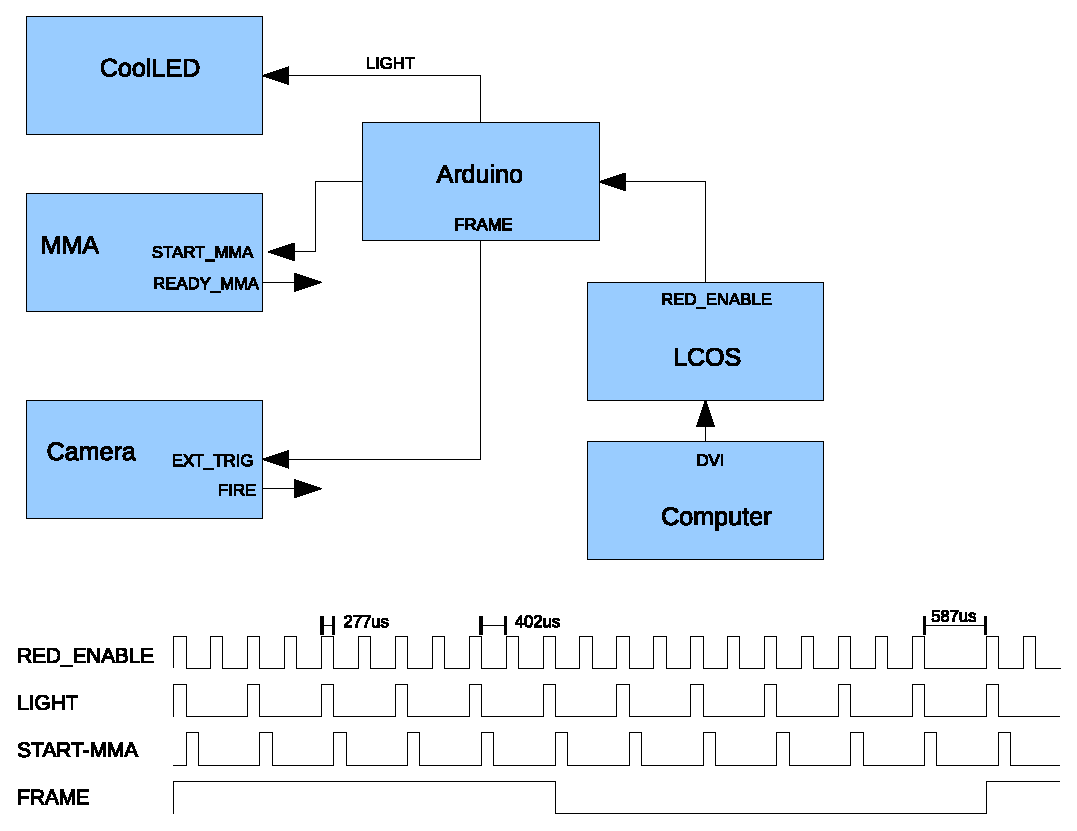
\includegraphics[width=12cm]{../dvi/trigger0}
  \caption{{\bf top:} Schematic of the electronic components of the
    system for the ``fast MMA'' trigger scheme. {\bf bottom:}
    Depiction of TTL trigger signals for this configuration. The
    \textsf{RED-ENABLE} signal is high, when the LCoS displays a
    bitplane. \textsf{LIGHT} enables the laser and \textsf{START-MMA}
    triggers the MMA, which displays an image after a delay of
    $\unit[850]{\mu s}$. The signal \textsf{FRAME} indicates the
    beginning of video frames and is necessary to start camera
    exposures at the right time.}
  \label{fig:trigger0}
\end{figure}


\section{Description of the trigger generation (slow MMA)}
\label{sec:dvi_slow}
The MMA and its controller are a prototype. The MMA can display images
from local storage with \unit[660]{Hz} but uploading one new image
from the computer roughly takes \unit[80]{ms}.

Therefore we switched to a different triggering scheme, where the
mirrors of the MMA are deflected during a full video frame of
\unit[16.66]{ms}. The MMA has a limited maximum duty cycle of
50\%. This means we have to drop every other frame from the graphics
card. If camera exposure times of \unit[16.66]{ms} are sufficient, we
have even doubled the duty cycle of the spatio-angular system to
$\unit[277]{\mu s}\times23\times\unit[60]{Hz}=0.38$. Note that we
loose the first bitplane due to the MMA's $\unit[850]{\mu s}$ load
delay.

The z-stage of the microscope can perform $\unit[1]{\mu m}$ steps in
\unit[20]{ms}. Therefore displaying two black images on the LCoS (and
capturing one of them) is sufficient to ensure that the stage is at
the next position.

The following code listing shows the Arduino microcontroller program,
that recovers the \textsf{VSYNC} signal from the pulse train on the
\textsf{RED-ENABLE} signal from the LCoS controller it generates
pulses with \unit[60]{Hz} on pin 13 that synchronize the MMA
controller.  {\small\label{fig:arduino-vsync}
\begin{verbatim}
// takes the lcos signal (train of 24 pulses, followed by a pause)
// and generates a trigger signal for the mma at the end of each train
// so for every DVI image (consisting of 24 bit planes) a different
// mma image can be shown. 

volatile unsigned int Ticks;    // holds the pulse count as .5 us ticks
// pin 8 takes signal from lcos
char icpPin = 8;                // this interrupt handler must use pin 8
volatile char bit_plane_change = 0;  // incremented whenever a 
                                     // different bitplane is displayed
char mma = 13;                  // output towards mma

ISR (TIMER1_CAPT_vect) // interrupt gets called when pin 8 changes
{
        if (!bit_is_set (TCCR1B, ICES1)) // was rising edge detected?
                TCNT1 = 0;      // reset the counter
        else {                  // falling edge was detected
                Ticks = ICR1;
                if (Ticks > 1000) {
                        bit_plane_change = 0;
                }
        }
        TCCR1B ^= _BV (ICES1);  // toggle bit value to trigger on the
                                // other edge
        if (bit_plane_change == 47) {
                digitalWrite (mma, HIGH);
        }
        else if (bit_plane_change == 0) {
                digitalWrite (mma, LOW);
        }
        bit_plane_change++;
}
void setup ()                   // run once, when the sketch starts
{
        pinMode (icpPin, INPUT);
        pinMode (mma, OUTPUT);
        TCCR1A = 0x00;     // COM1A1=0, COM1A0=0 => Disconnect Pin OC1
                           //                     from Timer/Counter 1
                           // PWM11=0,PWM10=0 => PWM Operation disabled
        TCCR1B = 0x02;     // 16MHz clock with prescaler means TCNT1
                           // increments every .5 uS (cs11 bit set)
        Ticks = 0;         // default value indicating no pulse detected
        TIMSK1 = _BV (ICIE1); // enable input capture interrupt for timer 1
}
int getTick ()
{
        int akaTick;      // holds a copy of the tick count so we can
                          // return it after re-enabling interrupts
        cli ();           // disable interrupts
        akaTick = Ticks;
        sei ();           // enable interrupts
        return akaTick;
}
char get_plane_change ()
{
        int aka;
        cli ();
        aka = bit_plane_change;
        sei ();
        return aka;
}
void loop () {}                 
\end{verbatim}
}

Finally we found a way to access the \textsf{VSYNC} signal on the LCoS
controller board by building an attachable circuit board with galvanic
isolation, making the above program obsolete.


\begin{figure}[!hbt]
  \centering
  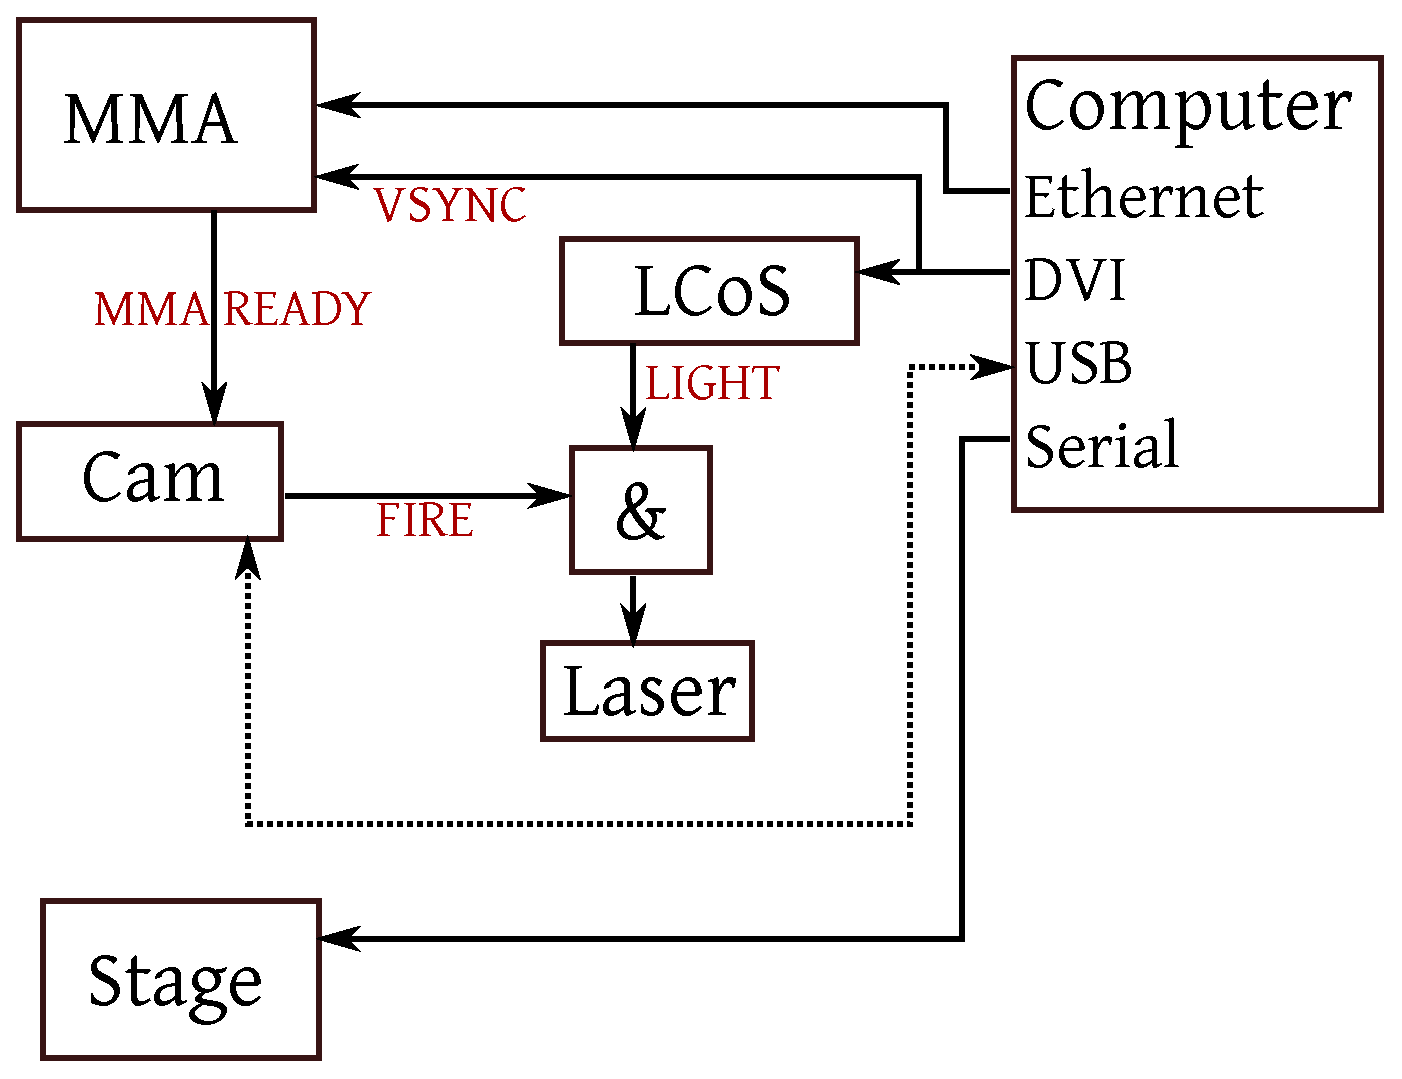
\includegraphics[width=8cm]{../dvi/09trigger}
  \caption{Schematic of the electronic system for the ``slow MMA''
    trigger scheme. The graphics card in the computer is the
    master. It generates images on the LCoS with \unit[60]{Hz}. The
    LCoS defines when the light can turn on but the Laser is only
    enabled, when the camera is integrating as well. The MMA selects
    only every second video frame from the graphics card and notifies
    the camera, when it has deflected its mirrors. The z-stage is controlled by the computer from within the display loop for the graphics card (synchronized with the signal \textsf{VSYNC}).  }
  \label{fig:09trigger}
\end{figure}



\begin{figure}[!hbt]
  \centering
  \includegraphics[width=12cm]{screen_logic_labels}
  \caption{Snapshot of the trigger signals for the ``slow MMA''
    configuration with a logic analyzer (Saleae Logic). The LCoS is
    the master, every second frame from the graphics card is
    integrated by the camera (which is running at \unit[30]{Hz}). The
    MMA has its mirrors tilted when the camera integrates, due to the
    delay of $\unit[850]{\mu s}$ the first image from the LCoS isn't
    collected in the exposure.}
  \label{fig:screen_logic_labels}
\end{figure}

\section{Verification of the synchronization}
In order to verify that the system is working, the graphics card is
displaying images with counters that incremented every frame (see
\figref{fig:fast4-no-first_cut}). As only every second image is
captured one would expect only odd counter numbers on the
camera. However, approximately every 400 images a jump of on or more
frames occurs. This problem can be traced back to the Steel Banks
Common Lisp\footnote{We used Common Lisp to develop most of our
  system. The main reason being an \unit[8]{s} initialization time in
  our camera's (Andor Clara) driver, that can't be disabled and
  hinders the C style edit--compile--run cycle.} garbage collector. A
garbage collection can take up to \unit[80]{ms}, which is not
sufficient for the required update rate of \unit[16]{ms}. Porting the
code to C fixes this issue.

\begin{figure}[!hbt]
  \centering
  \includegraphics[width=14cm]{fast4-no-first_cut}
  \caption{Montage of many camera images captured in sequence. The
    LCoS shows two frame counters. The bottom of the two numbers is
    reset at the beginning of the experiment and therefore counts
    $1,3,5,\ldots$, by design only every second image is
    captured. Occasionally a jump in the numbers was observed (see
    marked image: jump from 599 to 600) when the garbage collector
    ran. This was fixed by porting the code to C.}
  \label{fig:fast4-no-first_cut}
\end{figure}

The system is now able to capture images with a rate of \unit[30]{Hz}
with a constant integration time of \unit[16]{ms}.  An experiment has
been devised, that can capture stacks of sectioned data. We do not use
the MMA for angular control but rather displays white and every fourth
a black image. The LCoS displays three phases of a vertical grating
and a black image. When both displays show the black image, the stage
moves to the next slice. Capturing the slice and moving \unit[1]{$\mu
  m$} takes eight video frames. A stack with 10 slices can be acquired
in \unit[1.3]{s}. \figref{fig:dvi-mosaic}~left shows images of a 3D
distribution of \unit[2]{$\mu m$} beads in agar acquired with this
imaging protocol.

The right mosaic in \figref{fig:dvi-mosaic} shows a reapplication of
the same acquisition protocol. However, there the devices didn't start
exactly at the same time.

One problem is that the camera doesn't provide time stamps, which
would be helpful to measure the latency between issuing the
\textsf{StartAcquistion} command and when the camera actually starts
integrating.  Regarding the MMA, there is no specification of how long
\textsf{SLM-SetStartMMA} or \textsf{SLM-SetPictureSequence} take and
when the next incoming trigger is processed.

One solution to the problem would be to display a sequence of patterns
in the beginning of each experiment that would allow the system to
recover the offset between the devices. An example pattern could be
five white images on the MMA ($+++++$), two dark double images on
LCoS, one dark LCoS double image, two dark LCoS double images ($--+--$).

By analyzing the camera images one could then recover when the bright
image arrived. The same procedure could be applied for the MMA as
well. In that case we would display $+++++$ on the LCoS and $--+--$ on
the MMA. This solution is rather cumbersome. Therefore we didn't try
it and replaced the LCoS with one that contains local storage.

\begin{figure}[!hbt]
  \centering
  \includegraphics[width=10cm]{dvi-mosaic}
  \caption{{\bf left:} Sequence of images that was acquired while LCoS,
    MMA, z-stage and camera are running in sync. The camera is
    constantly running at \unit[30]{Hz} and the stage moves while a
    black mask is displayed on the MMA as well as the LCoS. The sample
    is a $\unit[2]{\mu m}$ yellow-green beads in agar {\bf right:}
    Same sequence of images should be displayed but the devices
    (camera, MMA and LCoS) do not start at the same time.}
  \label{fig:dvi-mosaic}
\end{figure}

\section{Conclusion}
The approach of sending data from the computer graphics card to the
LCoS by DVI would have its advantages but a synchronized start of
camera, MMA and LCoS proved to be too difficult or impractical.

If there was one display less, the approach would work perfectly fine.
Indeed we planned to build the optics using a spherical mirror and
bring conjugate planes of the pupil and the field (angular and spatial
control) next to each other on one LCoS.

Another approach to solving the problem, is to generate a trigger
pulse from within the frame rendering loop in the computer
software. This pulse would be generated synchronous to \textsf{VSYNC}
and could ensure that all devices start running with the same video
frame.

% talk with nice pictures /mnt/backup/safe-with-time/torben/safed/0321/talk/talk.lisp  amazingly i wrote this presentation in lisp!
% theory /mnt/backup/safe-with-time/torben/safed/0417
% WP6 D6.6 Report on DIC experiments /mnt/backup/safe-with-time/torben/safed/1125
\chapter{DIC}
\lstdefinelanguage{Maxima}{
keywords={addrow,addcol,zeromatrix,ident,augcoefmatrix,ratsubst,diff,ev,tex,%
with_stdout,nouns,express,depends,load,submatrix,div,grad,curl,%
rootscontract,solve,part,assume,sqrt,integrate,abs,inf,exp},
sensitive=true,
comment=[n][\itshape]{/*}{*/}
}
\lstset{language=Maxima}

\citep{Schwertner2008}

\begin{figure}[htbp]
  \centering
  \includegraphics[width=4cm]{dic-refocused-maximum-angle}
  \caption{}
  \label{fig:dic-refocused-maximum}
\end{figure}


\begin{figure}[htbp]
  \centering
  \includegraphics[width=4cm]{dic-setup}
  \caption{}
  \label{fig:dic-setup}
\end{figure}


\begin{figure}[htbp]
  \centering
  \includegraphics[width=4cm]{dic_prism-white-bg}
  \caption{}
  \label{fig:dic_prism-white}
\end{figure}


\begin{figure}[htbp]
  \centering
  \includegraphics[width=4cm]{mma-tilts}
  \includegraphics[width=4cm]{mma_dic-shear}
  \caption{}
  \label{fig:mma-tilts}
\end{figure}

\begin{figure}[htbp]
  \centering
  \includegraphics[height=4cm]{dic-setup-sketch}
  \caption{}
  \label{fig:dic-setup-sketch}
\end{figure}

\begin{figure}[htbp]
  \centering
  \includegraphics[width=4cm]{mma-dic-unadjusted}
  \caption{}
  \label{fig:mma-dic-unadjusted}
\end{figure}
\begin{figure}[htbp]
  \centering
  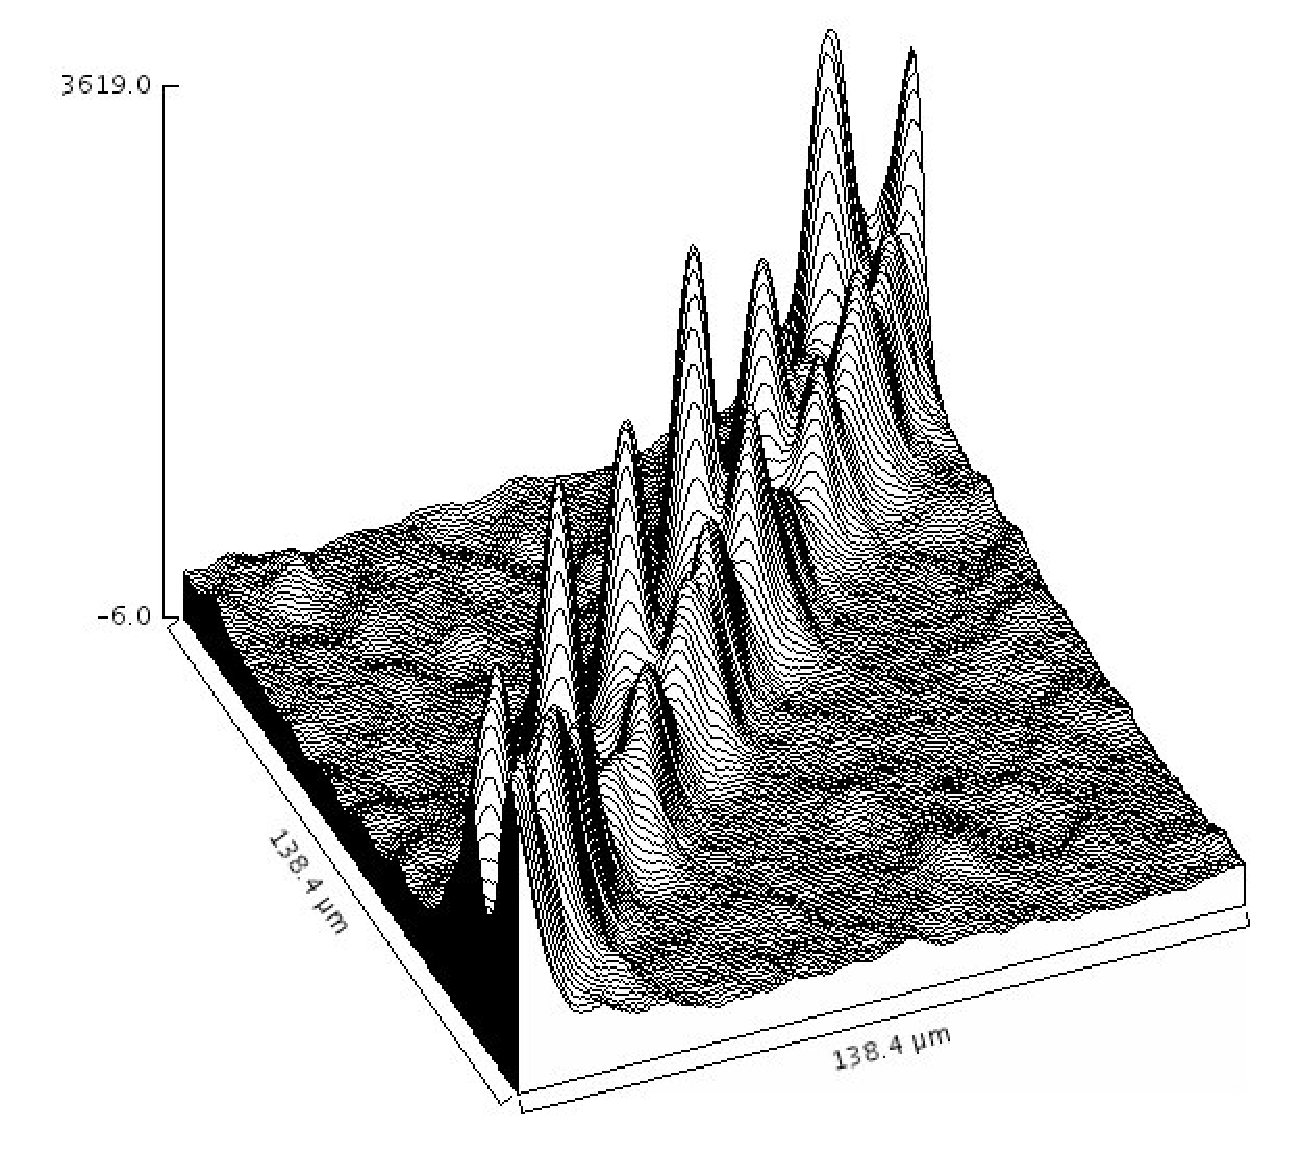
\includegraphics[width=4cm]{1checker-height}
  \caption{}
  \label{fig:1checker-height}
\end{figure}
\begin{figure}[htbp]
  \centering
  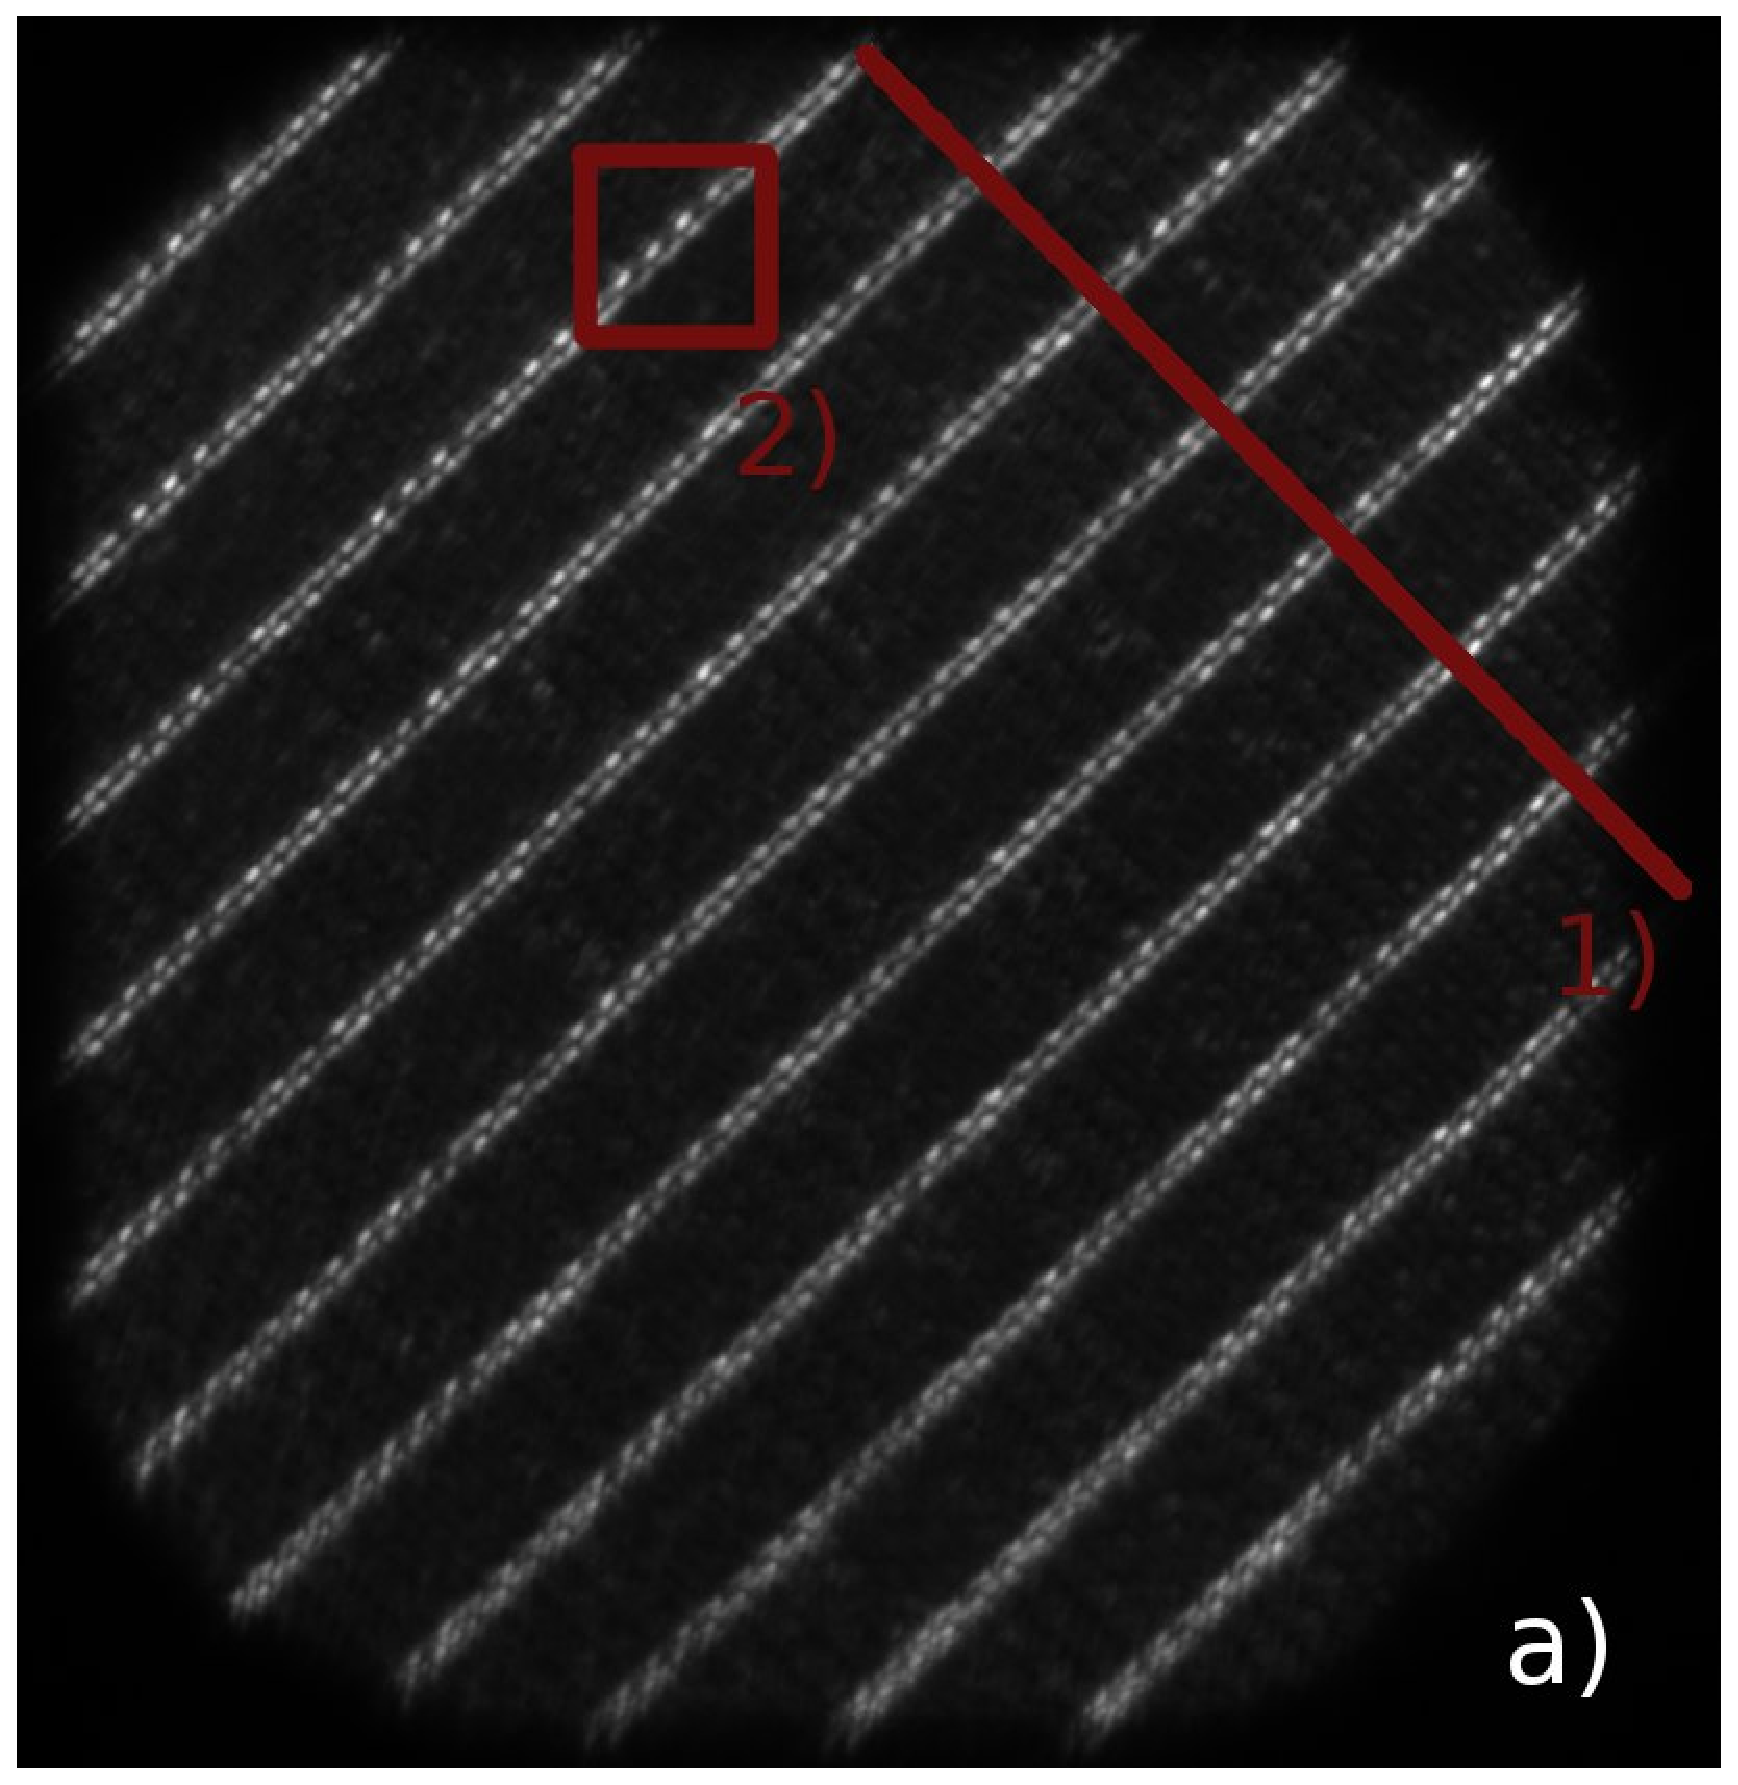
\includegraphics[width=4cm]{1checker}
  \caption{}
  \label{fig:1checker}
\end{figure}
\begin{figure}[htbp]
  \centering
  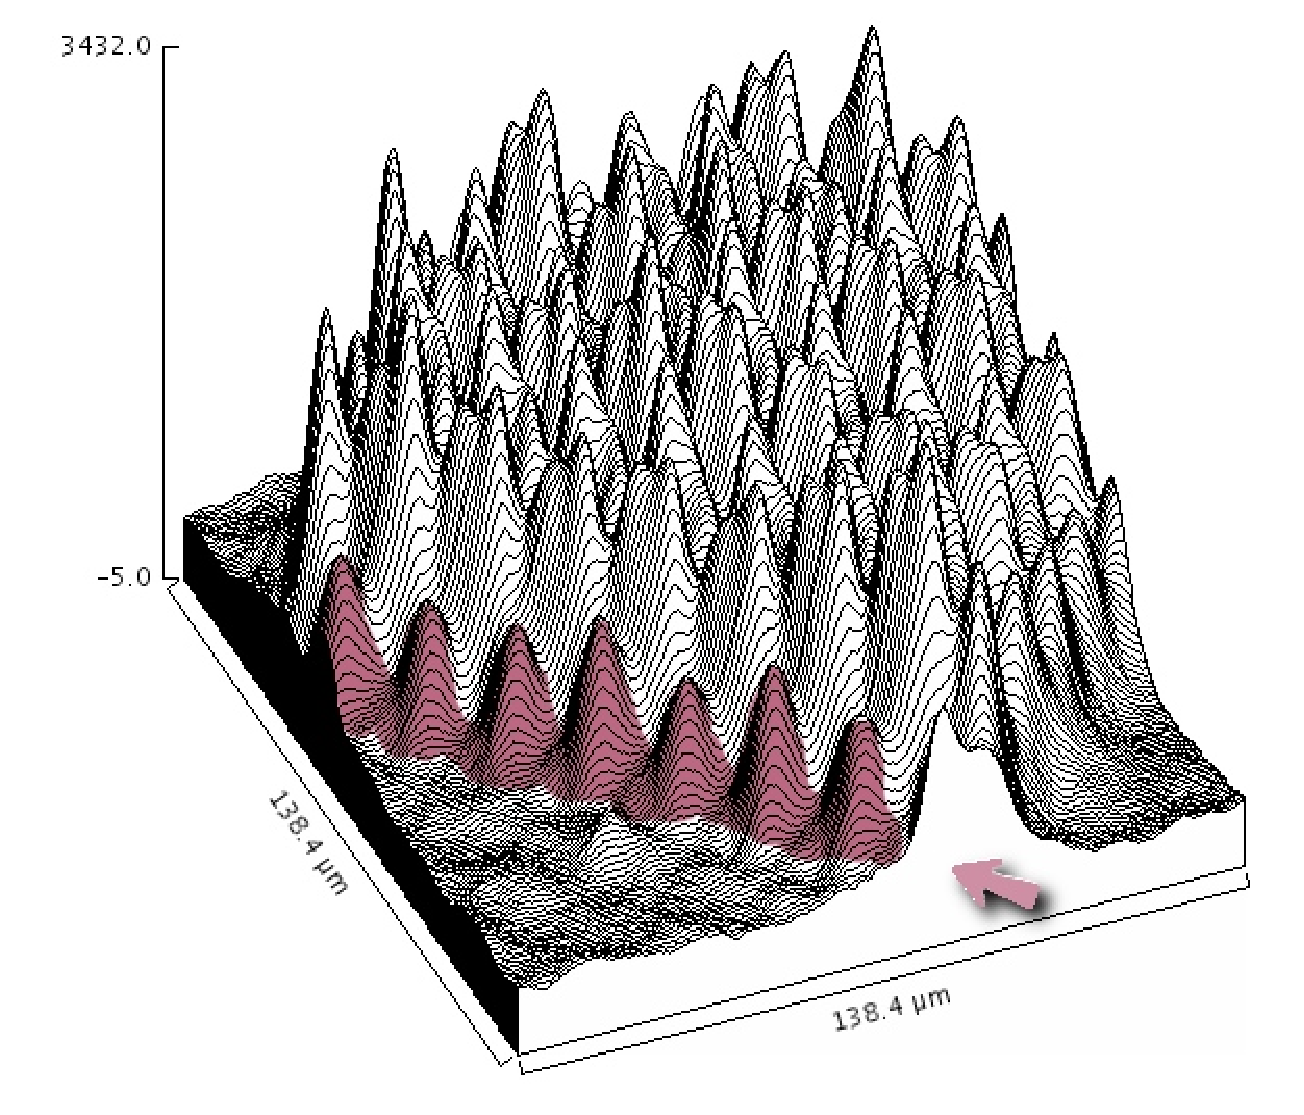
\includegraphics[width=4cm]{2checker-height-arrow}
  \caption{}
  \label{fig:height-arrow}
\end{figure}
\begin{figure}[htbp]
  \centering
  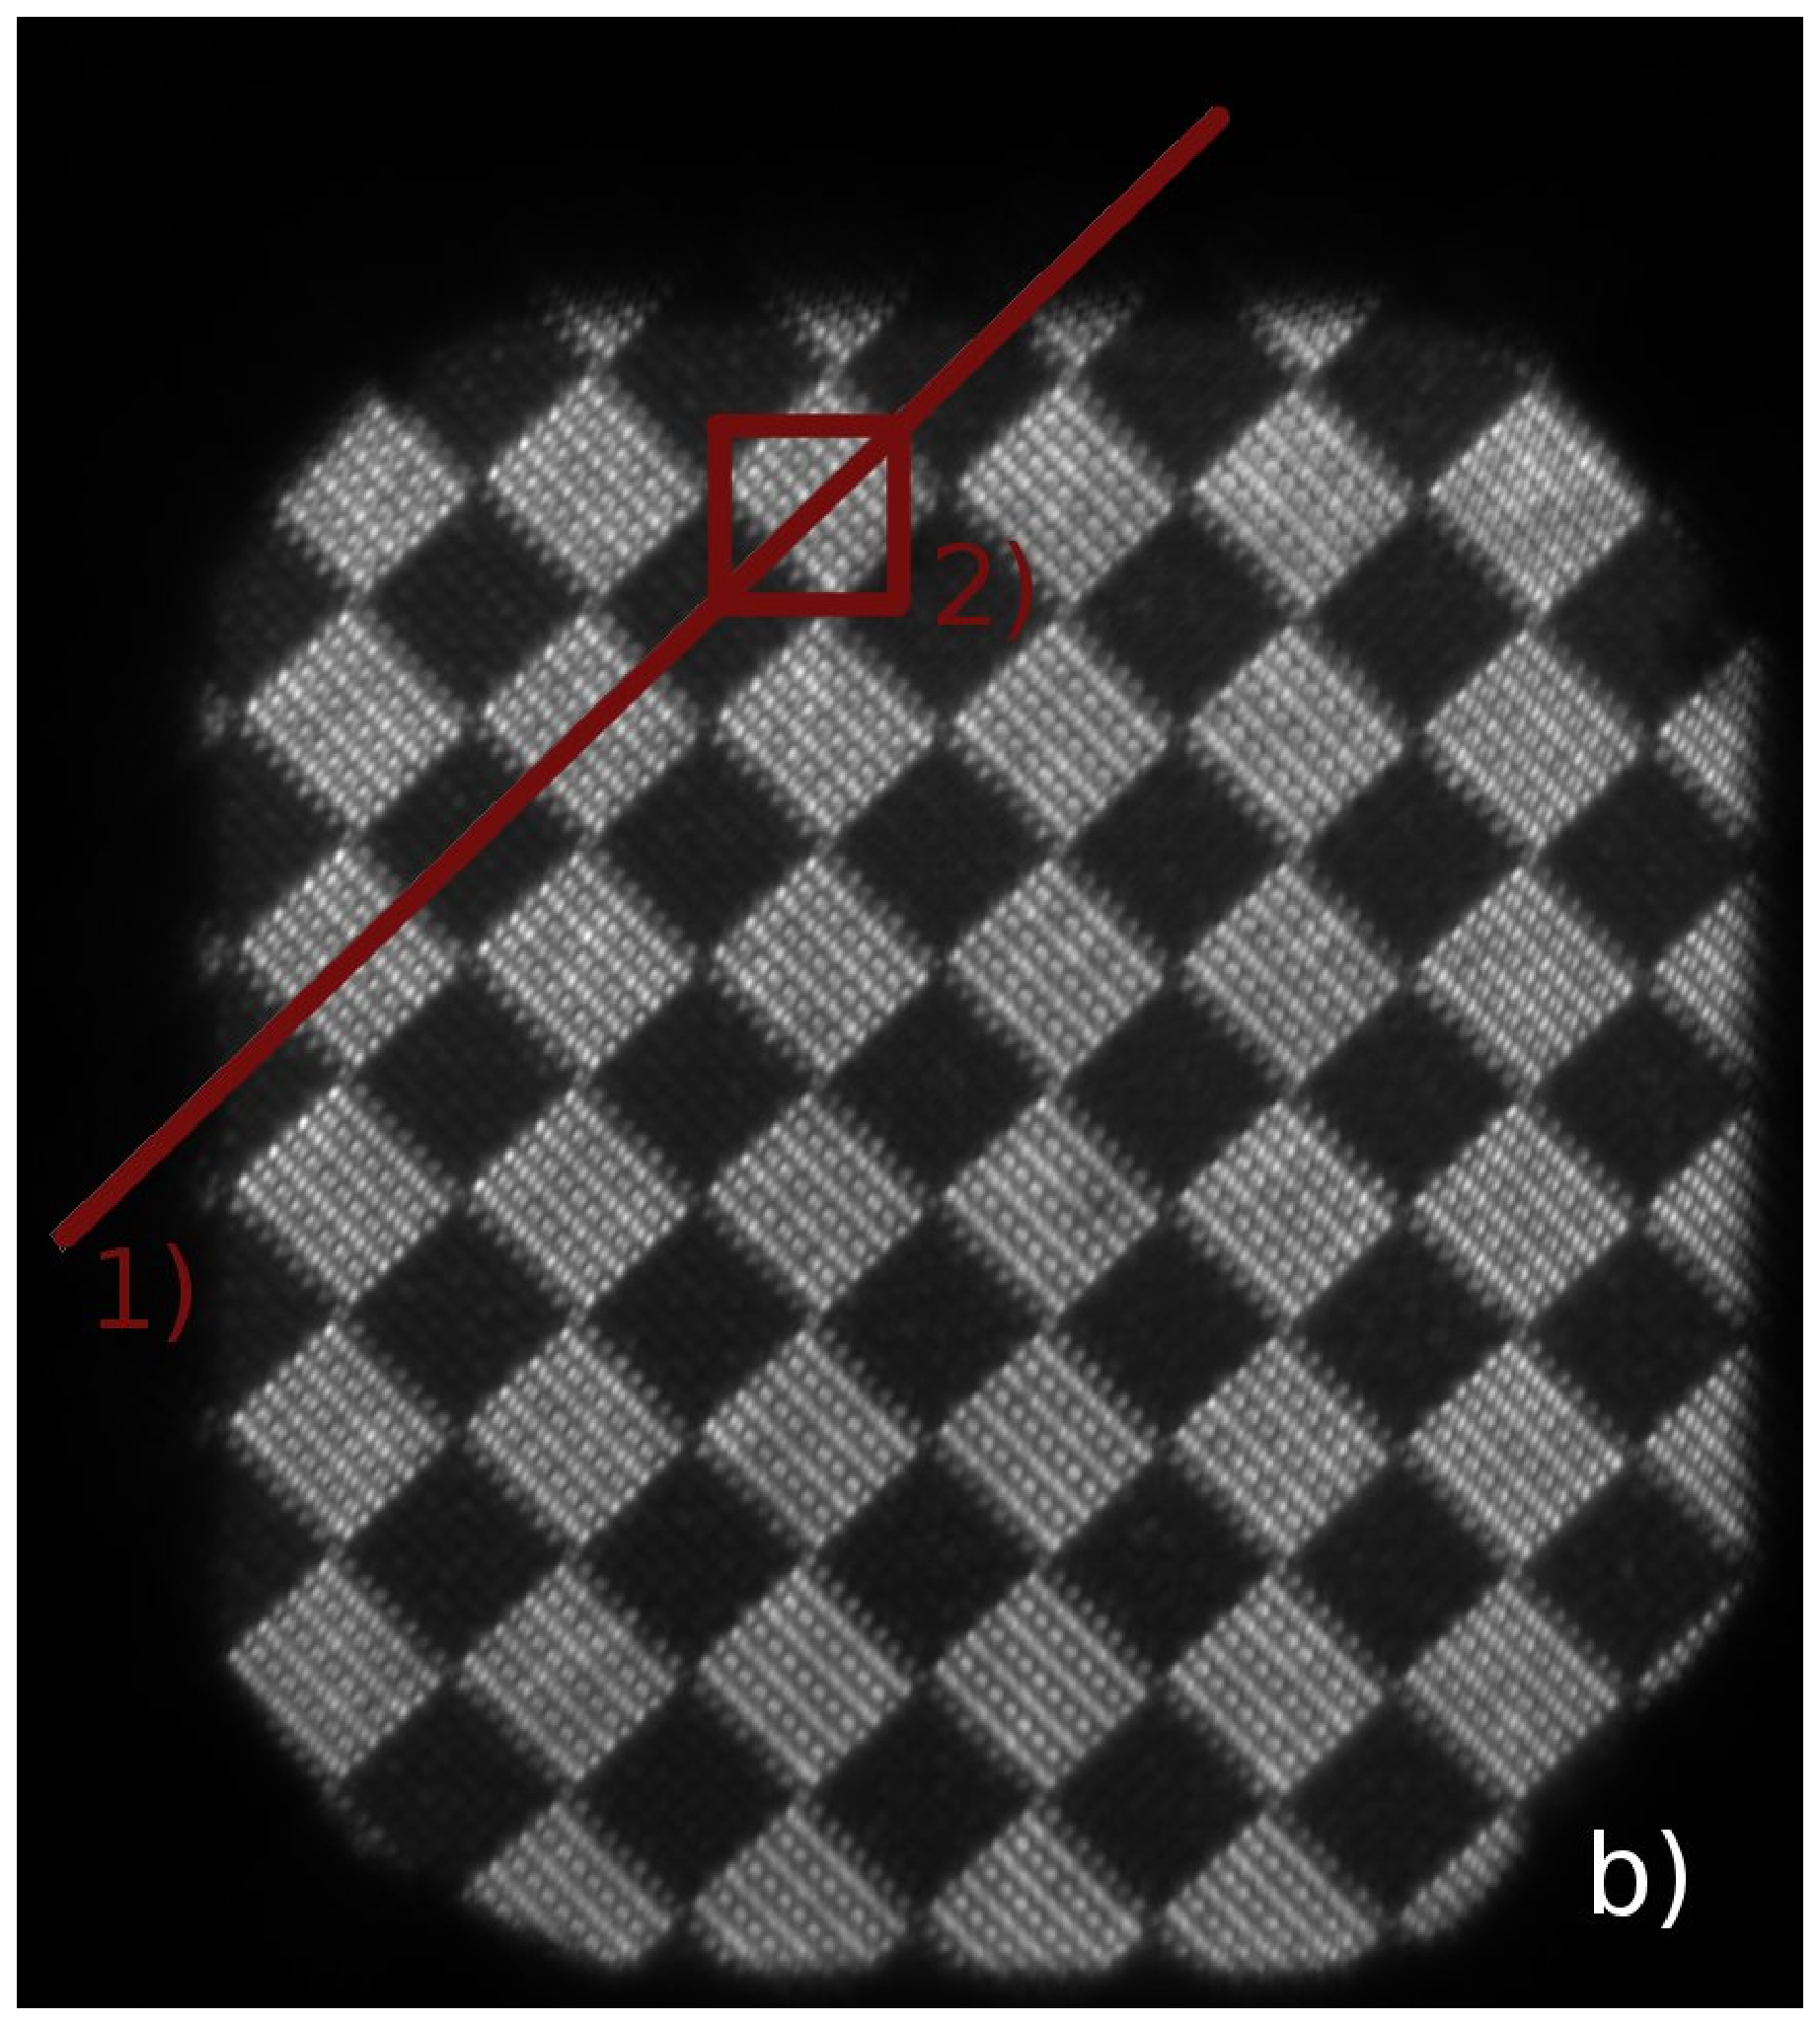
\includegraphics[width=4cm]{2checker}
  \caption{}
  \label{fig:2checker}
\end{figure}
\begin{figure}[htbp]
  \centering
  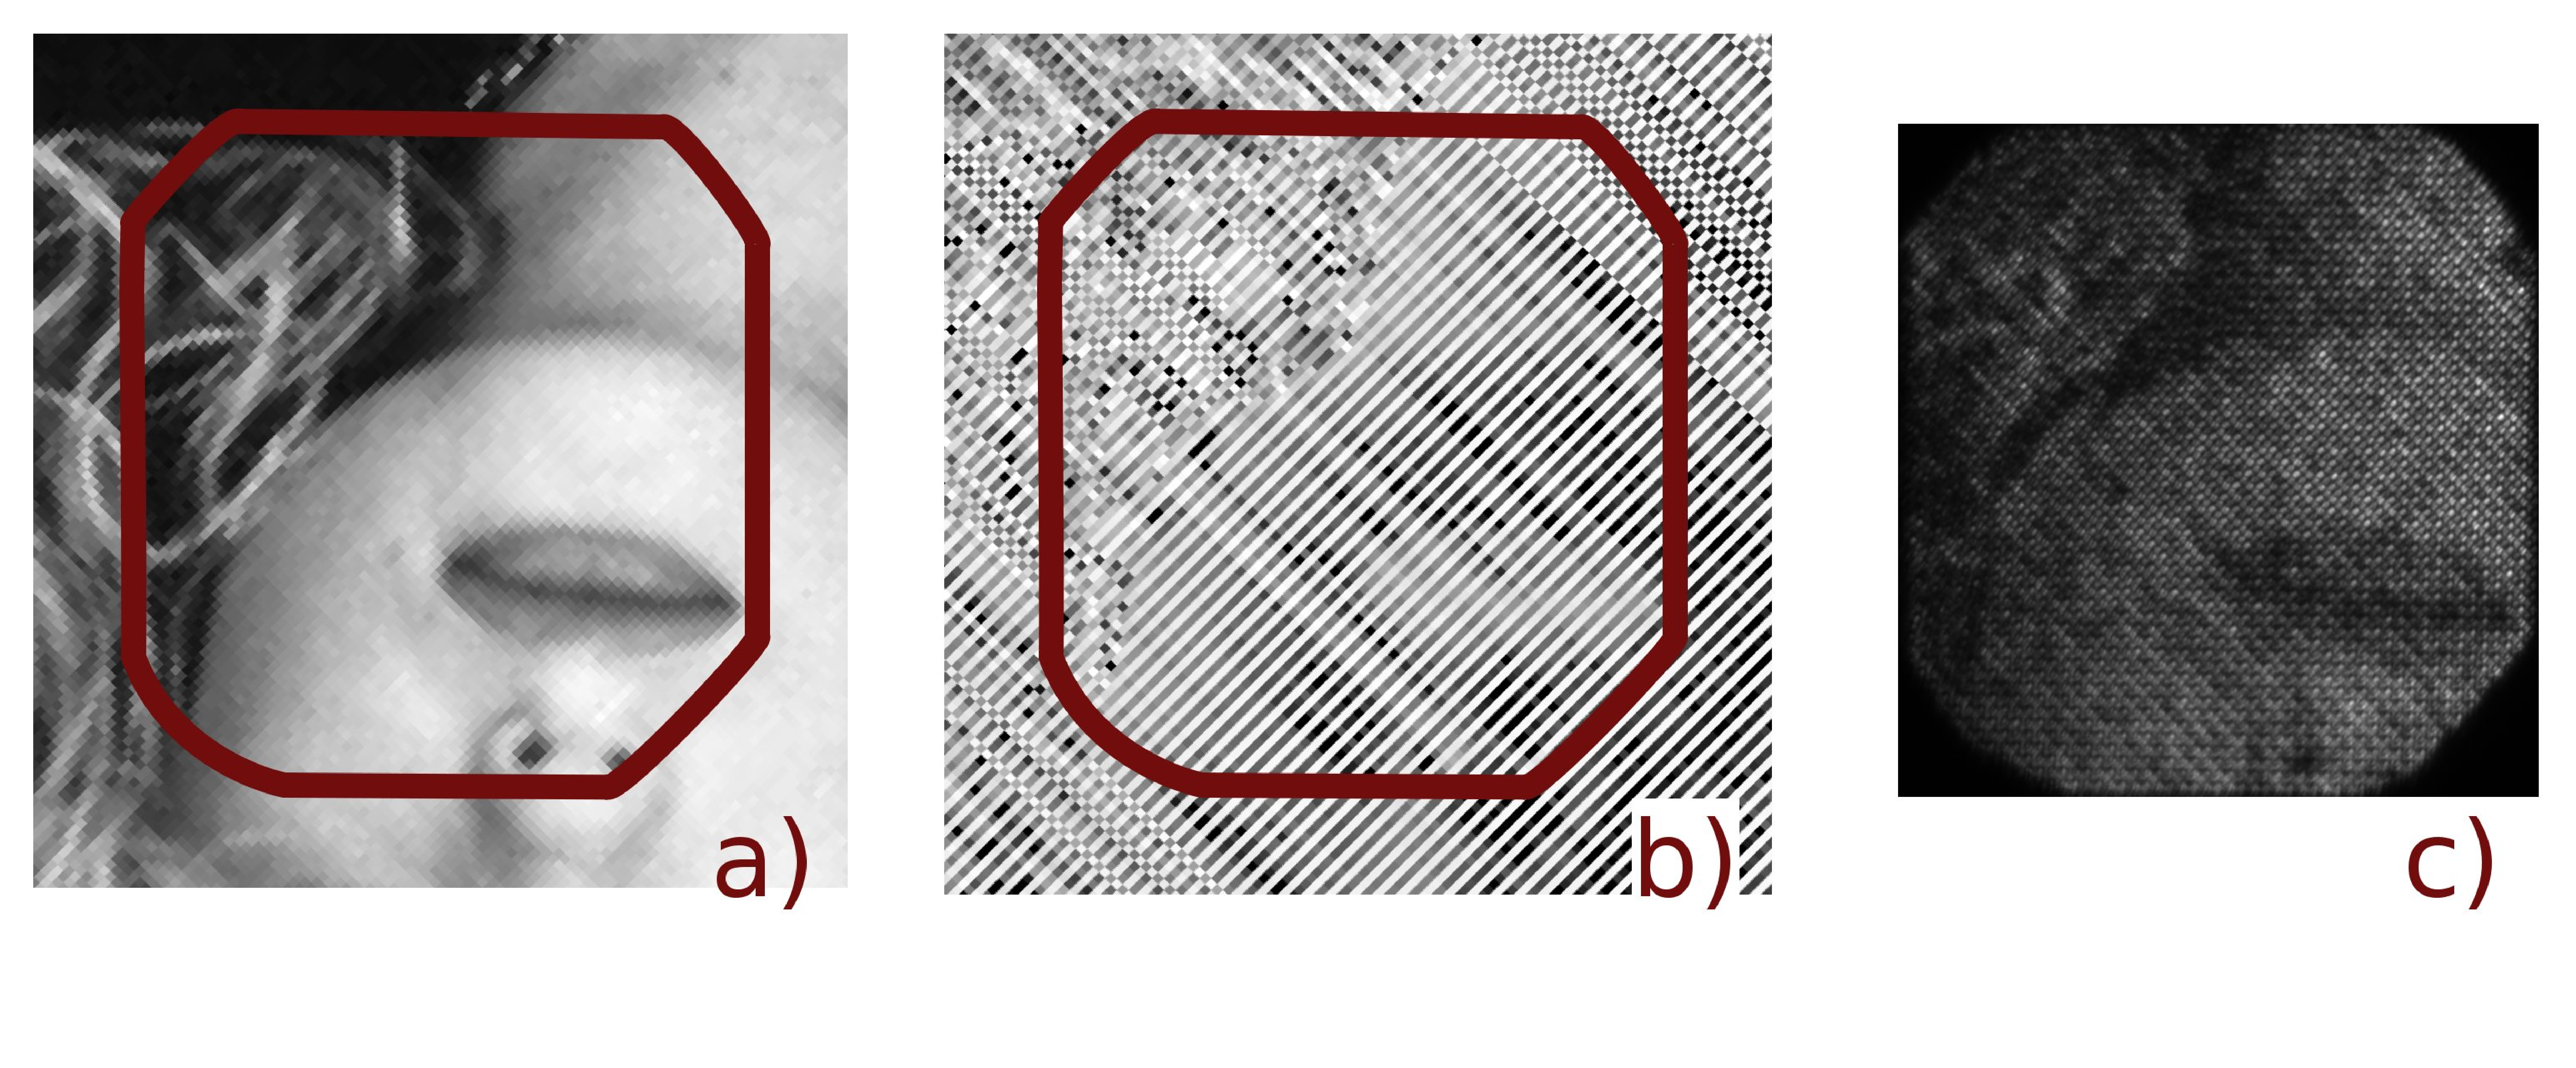
\includegraphics[width=4cm]{erika-detail}
  \caption{}
  \label{fig:detail}
\end{figure}

\begin{figure}[htbp]
  \centering
  \includegraphics[width=4cm]{erika-detail2}
  \caption{}
  \label{fig:detail2}
\end{figure}

\begin{figure}[htbp]
  \centering
  \includegraphics[width=4cm]{erika-streak-overview}
  \caption{}
  \label{fig:streak}
\end{figure}

\section{Abstract}
I describe the implementation of a simple raytracing algorithm for
uniaxial material.  The goal is to model a Wollaston prism and
estimate if it will be possible to use it for contrast enhancement of
a torsional micro-mirror array and to investigate what contrast we can
expect from the device.
\section{Description}
I want to design a Wollaston quartz prism that creates a split of
\unit[32]{mrad} between the two escaping beams.  A Wollaston prism is
a crystal plate consisting of two quartz wedges with an internal angle
$\alpha$. The right part of Figure 3 in \citep{Nomarski1960} shows the kind
of setup we intend to build. 
\begin{figure}[htbp]
  \centering
  \input{wollaston.eps_tex}
  \caption{Sketch of the raytrace through a Wollaston prism.}
\end{figure}
I take the names of the prisms from the Nomarski patent. I start the
trace with a beam that hits Q2 from the left. The optic axis of Q2 is
$\vect c_2=(0,1,0)^T$. It is perpendicular to the beam propagation. As
the ray enters the prism perpendicular to the front surface the
propagation angle doesn't change. However the ordinary beam is faster
than the extraordinary beam.

I calculate the refractive indizes of quartz with the formula given in
\citep{Ghosh1999}. For a wavelength of \unit[768]{nm} the refractive indices
are: $n_e=1.547916$ and $n_o=1.538998$.

At the contact surface between wedge Q1 and Q2 the ray direction for
ordinary and extraordinary beams change. Quartz is uniaxial
birefringent and optically active. Optical activity doesn't concern us
here it only has an important influence if the ray direction is in a
low angle to the optic axis (which will never occur in this Wollaston).

The calculation of the refracted wavevector and ray direction is
described in \citep{Lekner1991,Weidlich2008}. Here I implemented these
formulas in Maxima. I chose Maxima because I hope it will be easier to
switch to multiple precision which is necessary to calculate the phase
difference between rays. Apparrently not even 128-bit long-double
would be good enough for these calculations \cite{Lekner1991}. Knowing
the phase difference between the two beams is important to understand
if the prism will actually recombine zeroth and first order of the
micro-mirrors into a proper DIC image. I fear that the first order ray
might have a completely wrong phase leading to image artifacts and
very low contrast.

These two papers don't describe refraction at a
birefringent-birefringent interface. However I am not interested in
the exact Fresnel coefficients. I just start with one perfectly
polarized ray in Q1 and use the wavevector (the length $|\vect k_e|$
for $n_e(\theta)$) to calculate the direction in Q2 and the refractive
index there. I do this calculation twice. Once for the ray which is
polarized in the xz-plane and another time for the ray in the
yz-plane.  For the quartz-air interface I use the function raytrace2.
Its a copy of the birefringent solver but uses $n_e=n_o=1$. That's
easier than implementing a simple refraction formula for now.

The comments of the Maxima listing contain the results for an internal
wedge angle of 0.83 degrees. This angle was originally given to me by
the Comar polarization expert as an estimated angle needed to achieve
\unit[32]{mrad} between the exiting beams. Note that if my
calculations are correct it seems like he mixed up mrad and degree as
the angle between the two exiting beams is \unit[0.031]{degrees}.

\begin{lstlisting}
/*
uniaxial raytracer p0416/1991lekner_uniaxial.pdf
good repetition in p0415/2008weidlich_render-calcit.pdf
dispersion data for quartz  p0415/1999ghosh_quartz-calcite-dispersion-data.pdf
wollaston prism configuration for nomarski contrast (patent) Desktop2/NOMARSKI.pdf
*/

/* raytracer code according to 1991 lekner */

/* use a high precision */
showtime:false;
fpprec:800;
fpprintprec:25;
type:bfloat;

/* dispersion data from 1999 ghosh */
n_quartz_o2(l):=block(
  [a:1.28604141,
  b:1.07044083,
  c:1.00585997e-2,
  d:1.10202242,
  f:100,l2:l^2],
  a+b*l2/(l2-c)+d*l2/(l2-f));

n_quartz_e2(l):=block(
  [a:1.28851804,
  b:1.09509924,
  c:1.02101864e-2,
  d:1.15662475,
  f:100,l2:l^2],
  a+b*l2/(l2-c)+d*l2/(l2-f));

/* xi and phi give the direction of the optic axis
   theta is the angle of the incoming wavevector towards the surface normal
   n1 is the refractive index of medium for the incoming beam */
raytrace(lambda0,xi,phi,theta,n1):=block(
  [eo,ee,de,c,alp,bet,gam,k,kin,K,weg,q,q1,
  qo,No,Eo,so,d,qe,Ne,Ee,se,Eox,Eoy,Eoz,Eex,Eey,Eez,
  A,B,D,
  rss,rsp,tso,tse,
  qt,
  rpp,rps,tpo,tpe,
  ko,ke],
  eo:n_quartz_o2(lambda0),
  ee:n_quartz_e2(lambda0),
  de:ee-eo,
  /* orientation of optic axis */
  xi:xi*%pi/180,
  phi:phi*%pi/180,
  c:[sin(xi)*cos(phi),sin(xi)*sin(phi),cos(xi)],bfloat,
  c:c/sqrt(c.c),
  [alp,bet,gam]:c,
  /* incoming wavevector */
  n1:1,
  theta:theta*%pi/180,bfloat,
  k:2*%pi/lambda0,bfloat,
  kin:n1*k*[sin(theta),0,cos(theta)],
  [K,weg,q]:kin,
  q1:q,
  /* ordinary ray */
  qo:sqrt(eo*k^2-K^2),
  No:1/sqrt(bet^2*eo*k^2+(alp*qo-gam*K)^2),
  Eo:No*[-bet*qo,alp*qo-gam*K,bet*K],
  ko:[K,0,qo],
  so:ko/sqrt(ko.ko),
  /* ray direction se of extraordinary ray */
  d:eo*(ee*(eo+gam^2*de)*k^2-(ee-bet^2*de)*K^2),numer,
  qe:(sqrt(d)-alp*gam*K*de)/(eo+gam^2*de),
  Ne:No/k*1/sqrt(eo),
  Ee:Ne*[alp*qo^2-gam*qe*K,
         bet*eo*k^2,
         gam*(eo*k^2-qe^2)-alp*qe*K],
  ke:[K,0,qe],       
  se:[(alp*qe-gam*K)*(alp*qe*K-gam*(eo*k^2-qe^2))+bet^2*K*eo,
      bet*(alp*K+gam*qe)*(qe^2-qo^2),
      (alp*qe-gam*K)*(alp*qo^2-gam*qe*K)+bet^2*qe*eo*k^2],numer,
  se:se/sqrt(se.se),
  /* reflection and transmission coefficients for
  s-polarization at isotropic-birefringent interface */
  [Eox,Eoy,Eoz]:Eo,
  [Eex,Eey,Eez]:Ee,
  A:(qo+q1+K*tan(theta))*Eox-K*Eoz,
  B:(qe+q1+K*tan(theta))*Eex-K*Eez,
  D:(q1+qe)*A*Eey-(q1+qo)*B*Eoy,
  rss:((q1-qe)*A*Eoy-(q1-qo)*B*Eoy)/D,
  rsp:2*n1*k*(A*Eex-B*Eox)/D,
  tso:-2*q1*B/D,
  tse:-2*q1*A/D,
  /* coefficients for p-polarization */
  qt:q1+K*tan(theta),
  rpp:(2*qt/D)*((q1+qe)*Eox*Eey-(q1+qo)*Eex*Eoy),
  rps:2*n1*k*(qe-qo)*Eoy*Eey/D,
  tpo:2*n1*k*(q1+qe)*Eey/D,
  tpe:-2*n1*k*(q1+qo)*Eoy/D,
  [so,se,ko,ke]);

raytrace2(lambda0,xi,phi,theta,n1,n2):=block(
  [eo,ee,de,c,alp,bet,gam,k,kin,K,weg,q,q1,
  qo,No,Eo,so,d,qe,Ne,Ee,se,Eox,Eoy,Eoz,Eex,Eey,Eez,
  A,B,D,
  rss,rsp,tso,tse,
  qt,
  rpp,rps,tpo,tpe,
  ko,ke],
  eo:n2^2,
  ee:n2^2,
  de:0,
  /* orientation of optic axis */
  xi:xi*%pi/180,
  phi:phi*%pi/180,
  c:[sin(xi)*cos(phi),sin(xi)*sin(phi),cos(xi)],bfloat,
  c:c/sqrt(c.c),
  [alp,bet,gam]:c,
  /* incoming wavevector */
  n1:1,
  theta:theta*%pi/180,bfloat,
  k:2*%pi/lambda0,bfloat,
  kin:n1*k*[sin(theta),0,cos(theta)],
  [K,weg,q]:kin,
  q1:q,
  /* ordinary ray */
  qo:sqrt(eo*k^2-K^2),
  No:1/sqrt(bet^2*eo*k^2+(alp*qo-gam*K)^2),
  Eo:No*[-bet*qo,alp*qo-gam*K,bet*K],
  ko:[K,0,qo],
  so:ko/sqrt(ko.ko),
  /* ray direction se of extraordinary ray */
  d:eo*(ee*(eo+gam^2*de)*k^2-(ee-bet^2*de)*K^2),numer,
  qe:(sqrt(d)-alp*gam*K*de)/(eo+gam^2*de),
  Ne:No/k*1/sqrt(eo),
  Ee:Ne*[alp*qo^2-gam*qe*K,
         bet*eo*k^2,
         gam*(eo*k^2-qe^2)-alp*qe*K],
  ke:[K,0,qe],       
  se:[(alp*qe-gam*K)*(alp*qe*K-gam*(eo*k^2-qe^2))+bet^2*K*eo,
      bet*(alp*K+gam*qe)*(qe^2-qo^2),
      (alp*qe-gam*K)*(alp*qo^2-gam*qe*K)+bet^2*qe*eo*k^2],numer,
  se:se/sqrt(se.se),
  /* reflection and transmission coefficients for
  s-polarization at isotropic-birefringent interface */
  [Eox,Eoy,Eoz]:Eo,
  [Eex,Eey,Eez]:Ee,
  A:(qo+q1+K*tan(theta))*Eox-K*Eoz,
  B:(qe+q1+K*tan(theta))*Eex-K*Eez,
  D:(q1+qe)*A*Eey-(q1+qo)*B*Eoy,
  rss:((q1-qe)*A*Eoy-(q1-qo)*B*Eoy)/D,
  rsp:2*n1*k*(A*Eex-B*Eox)/D,
  tso:-2*q1*B/D,
  tse:-2*q1*A/D,
  /* coefficients for p-polarization */
  qt:q1+K*tan(theta),
  rpp:(2*qt/D)*((q1+qe)*Eox*Eey-(q1+qo)*Eex*Eoy),
  rps:2*n1*k*(qe-qo)*Eoy*Eey/D,
  tpo:2*n1*k*(q1+qe)*Eey/D,
  tpe:-2*n1*k*(q1+qo)*Eoy/D,
  [so,se,ko,ke]);

/* parameters: raytrace(lambda0,xi,phi,theta,n1) */
lambda0:.768;
k0:2*%pi/lambda0,numer;
/*        8.18123086872342 */
[so1,se1,ko1,ke1]:raytrace(lambda0,90,90,0,1),numer;
ne1:sqrt(ke1.ke1)/k0; /* 1.547916493897061 */
no1:sqrt(ko1.ko1)/k0; /* 1.538998122289932 ordinary is faster */
/* polarization of ordinary is perpendicular to the optic axis */
/* inner wedge angle */
alpha:0.83;
/* send light with polarization in xz-plane into second
   material (was ordinary in Q2 and is extraordinary in Q1) */ 
[weg,se2,weg2,ke2]:raytrace(lambda0,90,0,alpha,no1),numer;
se2; /* [.009466978585459387,0.0,.9999551871541356] note se2_x is positive */
ne2:sqrt(ke2.ke2)/k0; /* 1.547915706058689 */

/* send light with polarization in yz-plane into
   second material (was extraordinary and will be ordinary) */
[so2,weg,ko2,weg2]:raytrace(lambda0,90,0,alpha,ne1),numer;
so2; /* [.009412439124391275,0,.9999557020137091] */
ko2; /* [.1185110698410409,0,12.59034119351692] */
ko2/sqrt(ko2.ko2);
/* [.009412439124391275,0,.9999557020137091] same as so2 as expected */
no2:sqrt(ko2.ko2)/k0; /* 1.538998122289932 this is no as expected*/

/* these are the angles of the wavevector towards the normal of the
last surface. for xz-polarized light its not the ray-direction! */
theta2e:atan(ke2[1]/ke2[3])*180/%pi,numer; /* .5361939816441641 (xz) */
theta2o:atan(ko2[1]/ko2[3])*180/%pi,numer; /* .5393010000910526
                                           (yz same as ray direction) */
/* note: both are positive. yz-polarized light is refracted stronger */

/* xz-polarized light hits surface to air */
[weg,se3,weg2,ke3]:raytrace2(lambda0,90,0,theta2e,ne2,1),numer;
/* weg and weg2 should contain just the same information */

/* yz-polarized light hits surface to air */
[so3,weg,ko3,weg2]:raytrace2(lambda0,90,0,theta2o,no2,1),numer;

/* calculate the angles */

theta3e:atan(ke3[1]/ke3[3])*180/%pi,numer; /* .5361939816441641 (xz) */
theta3o:atan(ko3[1]/ko3[3])*180/%pi,numer; /* .5393010000910524 (yz) */
theta3o-theta3e; /* .003107018446888321 */
/* note: both angles are positive. the yz-polarized light is refracted
stronger */
\end{lstlisting}
% calibration of heo /mnt/backup/safe-with-time/torben/safed/y2009/0512
% measurement double plane /mnt/backup/safe-with-time/torben/safed/0525
% talk /mnt/backup/safe-with-time/torben/safed/0321/talk
\chapter{Holographic approach to spatio-angular illumination}
\begin{summary}
  Here we present an alternative system for spatio-angular control. It
  is based on a single phase-only LCoS. This simplifies electronic
  synchronization.
\end{summary}

\section{Introduction}
In this part we describe a very different approach that simplifies the
setup considerably.

\begin{figure}[!hbt]
  \centering
  \input{holo-setup3.eps_tex}
  \includegraphics[height=1cm]{hologram-disk}
  \caption{Schematic of the holographic spatio-angular microscope. A
    phase only LCoS in the intermediate image plane displays a grating
    and steers the first order into the back focal plane of the
    objective. Period and orientation define the angle of the
    illumination in the sample. Shape and contrast of the grating
    define the illuminated area and intensity of the illumination.}
  \label{fig:holo-setup3}
\end{figure}

\figref{fig:holo-setup3} shows a schematic of the setup. The main
component is a phase-only spatial light modulator in the intermediate
image plane. When nothing is displayed on the spatial light modulator,
it will reflect the Gaussian laser beam into a beam dump, so that
the light cannot enter the tubelens.

\section{Description of the holographic method}
The spatial light modulator is then programmed to display a phase
grating.  The direction and periodicity of a grating can be chosen
such that the first order is steered into any position on the back
focal plane. In the sketch the grating directs the first order into
the periphery of the back focal plane. Therefore the specimen will be
illuminated by light under a steep angle (not visible in
\figref{fig:holo-setup3} due to exaggerated focal length of
objective).

Decreasing the size of the grating will decrease the size of the
illuminated area in the object. Note that a grating of very small size
gives rise to a wide first order in the back focal plane, limiting the
possible angular control.
\subsection{Description of the experimental setup}
We use a HEO 1080 P High-Resolution LCOS Phase Only Spatial Light
Modulator (Holoeye, Berlin, Germany) to control the phase in the
intermediate plane. The light source is a \unit[473]{nm} DPSS diode
laser. It is coupled into a polarization maintaining fibre and
collimated by a \unit[150]{mm} lens with \unit[50]{mm} diameter.

The tube lens has \unit[300]{mm} diameter and the objective is a
$63\times/1.4$ with oil immersion.  For aligning the optical system a
sequence of device filling gratings was displayed at 60Hz. The
parameters of the grating were chosen such that the first order
describes a circle in the back focal plane.

\subsection{Description of the sample}
To show that the illumination angle of the light was indeed adjustable
a test sample was constructed. A slide and a cover slip were coated
with a thin fluorescent plane (see \figref{fig:holo-setup3}). The air
gap between the two fluorescent planes was approximately five
micrometres thick.

Imaging the fluorophore plane on the slide resulted in a haze of
background fluorescence stemming from the cover slip (see
\figref{fig:holo-meas}). Changing the illumination angle resulted in a
rotation of this haze as one would expect.
\begin{figure}
  \centering
  \includegraphics[width=12cm]{haze}
  \caption{Widefield images of a sample of two parallel fluorescent
    planes with varying azimuth angle of the illumination (numbers in
    in degree). One of the fluorescent planes is in focus, the other
    is imaged as an unsharp haze.}
  \label{fig:holo-meas}
\end{figure}

\section{ Characterization of the phase-only spatial light modulator}
\begin{summary}
  Here we measure the correspondence between displayed gray values and
  resulting phase difference on the Holoeye HEO 1080P spatial light
  modulator.
\end{summary}
We use a similar setup as given in the manual \citep{Holoeye2006}.
\begin{figure}[!hbt]
  \centering
  \includegraphics[width=16cm]{sketch}
  \caption{Setup for calibrating the transfer function of the phase
    SLM. We will establish, which gray values correspond to what phase
    delay. The light from a polarization maintaining single mode fibre
    is circularly polarized by a $\lambda/4-$plate and a polarizer is
    then used to select the optimum polarization direction. The
    Fraunhofer diffraction pattern of light, which has been reflected
    from the device, is captured with a fast camera. (The display's
    cable would come out at the top, perpendicular to the paper
    plane.)}
  \label{fig:holo-calib}
\end{figure}
The SLM is illuminated with a parallel linearly polarized wave
front. The plane of vibration of the electric field is in the paper
plane.

The SLM displays two vertical bars. The left bar shows black (0) and
the upper bar displays a gray value that is varied for the
measurement.  The beam has a circular shape and a (sufficiently)
constant intensity distribution. The beam is centred on the line
between the two bars of different phase. 
\subsection{Numerical simulation}
The minima of the diffraction pattern in the Fourier plane (on the
camera) move proportional to the phase difference between the two
parts of the display (see \figref{fig:holo-theory}).
\begin{figure}[!hbt]
  \centering
  \includegraphics[width=12cm]{theory}
  \caption{Theoretical simulation of the Fraunhofer diffraction
    pattern for varying phase difference between the two sides of the
    display.}
  \label{fig:holo-theory}
\end{figure}
For the simulation we calculated the Fourier transform of a phase
image with a geometry as shown in the top left image in
\figref{fig:holo-theory}.  The three images on the right show the
Fraunhofer diffraction patterns of this (reflective) phase image for
three different values of the phase difference between the half
circles. The position of the minimum changes proportionally to the
phase difference. Therefore we can measure the position of the extrema
to determine the relationship between gray value and phase difference
(the transfer function of the device).

\subsection{Measurement}
The result of this measurement is shown in the top of
\figref{fig:holo-transfer}
(horizontal section through centre of
the Fourier pattern against gray value)
\begin{figure}[!hbt]
  \centering
  \includegraphics[width=16cm]{measure}
  \caption{{\bf top:} horizontal sections through the Fraunhofer
    diffraction pattern on the camera are plotted as columns. The
    displayed gray value is plotted as the x-axis. {\bf bottom:} Time
    variation of the phase, when a constant value of 170 is shown. The
    phase fluctuates considerably.}
  \label{fig:holo-transfer}
\end{figure}
The measurement shows that a phase difference of $2\pi$ can be induced
for a sufficiently high gray value. However we observe significant
noise for the phase measurements.  There are jumps in the data that
amount to several 10 gray values. 

To analyze this effect further a fast camera (mvBlueFox 102G, 2400 Hz,
$200\times4$ region of interest, $\unit[ 6]{\mu m}$ pixel size) was
used to image the Fourier pattern with a high time resolution.  The
bottom image in \figref{fig:holo-transfer} displays 1000 horizontal
line sections over the centre of the Fourier plane. In the beginning,
both half circles were displaying a gray value of zero. Then the right
half circle was suddenly set to 170. The transient occurs quite fast
but then there is a waveform with 5 peaks that repeats with 50 Hz (the
refresh rate of the display).

The measurement suggests that the phase difference of the Holoeye SLM
is varying significantly over time. In order to improve the
performance for displaying computer generated holograms we could
trigger the laser only for a short time before a new frame will be
displayed.

From other experiments we know that there is also cross talk between
the pixels, i.e. if a fine grating is displayed, the displayed phase
contrast is lower than for a coarser grating.
\section{Conclusion}
With our prototype system we showed that it is possible to use the
phase-only SLM to achieve angular and spatial control of the
illumination. Further work would be necessary to optimize the grating
fine structure in order to direct more light is directed towards the
first order (blazing).

Compared to the MEMI system a lot less synchronization between devices
is necessary. However, this technique is only possible with coherent
illumination. Furthermore there is no inherent advantage in the
holographic method as light from dark areas is sent into a beam stop
and is lost as in the MEMI system.

It might be possible to build a system using a kinoform element (two
phase holograms in different positions). This would allow to redirect
light from dark areas into bright areas leading to a much more
efficient system. A different display device with less cross talk
and fluctuations would be advisable for this.


\renewcommand{\(}{\left(}
\renewcommand{\)}{\right)}
\chapter{Equidistant spiral sampling}
\begin{summary}
  In our system the MMA is imaged into the circular back focal plane
  of the microscope objective. Here we propose a method of storing
  images of circular apertures in its linear frame buffer.
\end{summary}
\section{Archimedes Spiral}
An Archimedes spiral in polar coordinates $(r,\theta)$ is defined like
this:
\begin{align} \label{eqn:def}
  r(\theta)=a\,\theta.
\end{align}
The step height $h$ of the spiral is constant and given by
\begin{align}
  h=\abs{r(\theta)-r(\theta+2\pi)}=r(2\pi)=2\pi a.
\end{align}
We would like to distribute circular windows at equidistant points
along the spiral \citep{Ahn1986}.
\section{Equidistance sampling}
We want to start sampling in the centre at $r(0)=0$ and sample the arc
length of the spiral with equidistant points. The arc length of an
Archimedes spiral is \citep{Weisstein}:
\begin{align} \label{eqn:arclength}
  s(\theta)=\frac{a}{2}\(p\,\theta + \log(p\,\theta)\)\quad\textrm{with}\quad
  p=\sqrt{1+\theta^2}.
\end{align}
The arc length $\Delta s$ between successive points along the spiral
should be equal to the step height $h$. Starting from the central
point $\theta_0=0$ the arc length where to sample the $i-$th point can
be obtained by inverting equation \eqref{eqn:arclength}:
\begin{align}
  \theta_i=\theta(i\,\Delta s).
\end{align}
This inversion can be done efficiently with Newton iteration:
\begin{align}
  x_0&=1,\\
  x_{n+1}&=x_n-\frac{f(x)}{f'(x)}.
\end{align}
Here we introduce the function $f(\theta)$ that vanishes at a given arc
length $s$ and its derivative $f'(\theta)$:
\begin{align}
  \label{eqn:f}
  f(\theta)&=\frac{a}{2}\(p\,\theta+\log(p\,\theta)\)-s,\\
  f'(\theta)&=\frac{\partial f(\theta)}{\partial \theta}=
  \frac{a}{2}\frac{(1+2\theta^2)(1+p\theta)}{p^2 \theta}.
\end{align}
\section{Filling the back focal plane}
We want to find the coordinates of equally distributed sampling points
along the arc length inside of a circle with radius R. We put the
first sampling point $\theta_0=0$ in the centre and the last point
$\theta_n$ on the periphery of the circle. By definition
\eqref{eqn:def} of the spiral we know
\begin{align}
  \theta_n=R/a.
\end{align}
Now we obtain the arc length $s(\theta_n)$ of the spiral contained
inside the circle via \eqref{eqn:arclength}. Dividing by the number of
sub-intervals gives the appropriate sampling step $\Delta s =
s(\theta_n)/(n-1)$.

Note that we are only interested in solutions with $\Delta s=h$. We
want the sampling step to be equal to the step height $h=2\pi a$ of
the spiral. We therefore need to find the zero of the function:
\begin{align} \label{eqn:g}
  g(a)&=\frac{s(\theta_n)}{n-1}-2\pi a\\
  &=\frac{a}{2}\frac{p\theta_n+\log p\theta_n}{n-1}-2\pi a\\
  &=\frac{a}{2}\frac{\sqrt{1+\frac{R^2}{a^2}}\frac{R}{a}+
    \log\(\sqrt{1+\frac{R^2}{a^2}}\frac{R}{a}\)}{n-1}-2\pi a.
\end{align}
We know $a\not =0$ therefor we can transform the function to simplify
its derivative:
\begin{align} \label{eqn:g1}
  g_1(a)&=\underbrace{\sqrt{1+\frac{R^2}{a^2}}}_{p_1}\frac{R}{a} 
  +\log\(\sqrt{1+\frac{R^2}{a^2}}\frac{R}{a}\)-4\pi (n-1),\\
  g_1'(a)&=-\frac{R^3}{p_1}\frac{1}{a^4}-\frac{R^2}{p_1^2}\frac{1}{a^3}-R
    p_1\frac{1}{a^2}-\frac{1}{a}.
\end{align}
Newton's method can be used to find the zero $a_0$ of $g(a)$. Then
$\Delta s$ can be obtained and the circle drawn.

% for i in *.pgm ; do potrace $i ;done
\begin{figure}[h]
  \begin{center}
    \includegraphics[width=.3\columnwidth]{../app_spiral/o0030}
    \includegraphics[width=.3\columnwidth]{../app_spiral/o0100}
    \includegraphics[width=.3\columnwidth]{../app_spiral/o0200}
    \includegraphics[width=.3\columnwidth]{../app_spiral/o0300}
    \includegraphics[width=.3\columnwidth]{../app_spiral/o0400}
    \includegraphics[width=.3\columnwidth]{../app_spiral/o1024}
  \end{center}
  \caption{Equidistant sampling of a circle of the same radius
    $R=128$ with different number of points (from top left to bottom
    right: 30, 100, 200, 300, 400, 1024).}
\end{figure}

\section{Improvement for sampling with disks}
It is useful to modify the filling formula \eqref{eqn:g} such, that
disks with radius $r_s=\alpha\Delta s/2$ on the sample points don't
overlap the periphery of the big circle. Again we have $\theta_n=R/a$ but $R$ is smaller than the back focal plane radius $R_B$:
\begin{align}
  R=R_B-r_s.
\end{align}
Thus we can define the equivalent to \eqref{eqn:g1}:
\begin{align}
  \begin{split}
  g_2(a)&=\overbrace{\sqrt{1+\frac{(R_B-\pi\alpha a)^2}{a^2}}}^{p_2}
  \frac{R_B-\pi\alpha a}{a}+
  \log\(\sqrt{1+\frac{(R_B-\pi\alpha a)^2}{a^2}}\frac{R_B-\pi\alpha a}{a}\)\\ 
  &-4\pi (n-1),\end{split}\\
  g_2'(a)&=
  -\frac{R^3}{p_2}\frac{1}{a^4}
  -\(\frac{\pi\alpha R^2}{p_2}+\frac{R^2}{p_2^2}\)\frac{1}{a^3}
  -\(R p_2+\frac{\pi\alpha R}{p_2^2}\)\frac{1}{a^2}-\(\pi\alpha p_2+1\)\frac{1}{a}+\frac{\pi\alpha}{R}.
\end{align}


\begin{figure}[h]
  \begin{center}
    \includegraphics[width=.3\columnwidth]{../app_spiral/q0030}
    \includegraphics[width=.3\columnwidth]{../app_spiral/q0100}
    \includegraphics[width=.3\columnwidth]{../app_spiral/q0200}
    \includegraphics[width=.3\columnwidth]{../app_spiral/q0300}
    \includegraphics[width=.3\columnwidth]{../app_spiral/q0400}
    \includegraphics[width=.3\columnwidth]{../app_spiral/q1024}
  \end{center}
  \caption{A back focal plane of radius 100 is filled with equidistant
    spiral sampling, ensuring that the outermost disk is contained
    inside. The number of disks are (from top left to bottom right):
    30, 100, 200, 300, 400, 1024.}
\end{figure}

\section{Discussion}
It is possible to distribute sample points along a spiral over the
back focal plane. However, there doesn't seem to be any advantage to
placing the circles nodes of a polar grid. Indeed the spiral sampling
is actually worse because for high angles the circles are either cut
off or quite a large part of the BFP is not
covered. 

We believe hexagonal sampling \citep{Middleton2001} will be a better
alternative. It provides easy access to nearest neighbours and a
natural hierarchy.



%% FindRoot[{a x == R, a/2 (Sqrt[1+x^2]x+Log[Sqrt[1+x^2]x]) == n * 2 pi a + R/a}, {{x, 1}, {a, 1}}]

%% Weisstein, Eric W. "Archimedes' Spiral." From MathWorld--A Wolfram
%% Web Resource. http://mathworld.wolfram.com/ArchimedesSpiral.html

%% http://en.wikipedia.org/wiki/Newton's_method

%% multidimensional newton method
%% http://math.fullerton.edu/mathews/n2003/NewtonSystemMod.html

%\chapter{Construction of term symbols for molecular orbitals}
\label{sec:app_term}

The symmetric linear combination of the $1s$-orbitals of two atoms $A$
and $B$ is
\begin{align*}
  \sigma_g1s=\frac{1}{\sqrt2}(\sigma 1s_A+\sigma 1s_B).
\end{align*}
$\sigma_u$ is constructed as the difference of the two atomic
orbitals.  In general the symmetric molecular orbital $\sigma_g$ is
more stable as the electrons have a higher probability to be between
the nuclei.  The following quantum numbers describe the molecular wave
function:
\begin{description}
\item[$\Lambda\ ..$]
      
  Defined by $\mathbf{L}_z=\Lambda\hbar=|\sum\lambda_i|\hbar$ with
  projection $\lambda_i$ of the orbital angular momentum
  $\mathbf{l}_i$ of electron $i$ onto the nuclear axis. $\Lambda$ can
  take the values $0,1,2,\ldots$ and one writes the term symbols
  $\Sigma,\Pi,\Delta,\ldots$.
      
\item[$S\ ..$]
      
  Spin of all electrons $S=\sum\mathbf{m}_{si}$ in the molecular
  orbital.
      
\item[$\Omega\ ..$]
      
  Electronic angular momentum in direction of the nuclear axis.
      
\end{description}
These numbers are combined into the term symbol like this:
$\boxed{{}^{2S+1}\Lambda_\Omega}$.  Additionally one writes
e.g. $\Sigma^+$ if the molecular function is symmetric when mirrored
at a plane through the nuclei.  Furthermore one writes $\Sigma_g$ if
the sign of wave function stays the same when the molecule is inverted
at the point of symmetry.
    
Here are two examples of ``decoding'' the term symbols describing wave
functions of the hydrogen molecule:
    
\begin{description}
\item[$\sigma_g\sigma_g^1\Sigma_g^+$:]
      
  $\lambda_1=1,\ \lambda_2=-1,\ s_1=+,\ s_2=-$
      
  $\Lambda=|\lambda_1+\lambda_2|=|1-1|=0,\ S=s_1+s_2=0$
      
\item[$\sigma_g\pi_u^1\Pi_u$:]
      
  $\lambda_1=1,\ \lambda_2=-2,\ s_1=+,\ s_2=-$
      
  $\Lambda=|1-2|=1,\ S=0$
      
\end{description}

\bibliographystyle{abbrvnat}
%\bibliography{../state-of-art}
\bibliography{../All}
\end{document}


%%% Local Variables: 
%%% mode: latex
%%% TeX-master: t
%%% End: 
